\documentclass[12pt]{ociamthesis}

\usepackage[utf8]{inputenc}
\usepackage[english]{babel} % ty­po­graph­i­cal and hy­phen­ation rules
\usepackage{amsmath, amsthm, amsfonts}  % loads AMS packages
\usepackage{amssymb}  % provides support for some characters
\usepackage{hyperref} % provides automatic reference types and hyperlinks
\usepackage[noabbrev,capitalize]{cleveref}  % provides automatic reference types
\usepackage{tikz}
\usepackage{mathtools}  % extends amsmath; used in definition of \diag; remove?
%\usepackage{graphicx}  % already loaded by ociamthesis.cls
%\usepackage{array} % defines extra tabular environments
%\usepackage{ifthen}  % already loaded by ociamthesis.cls

\theoremstyle{plain}
\newtheorem{theorem}{Theorem}
\newtheorem{proposition}{Proposition}
\newtheorem{lemma}{Lemma}
\newtheorem{corollary}{Corollary}

\theoremstyle{definition}
\newtheorem{definition}{Definition}[section]

\theoremstyle{remark}
\newtheorem*{remark}{Remark}
\newtheorem{example}{Example}

%BEGIN_MACRO
\makeatletter
\newcommand{\mytag}[2]{%
  \text{#1}%
  \@bsphack
  \protected@write\@auxout{}%
         {\string\newlabel{#2}{{#1}{\thepage}}}%
  \@esphack
}
\makeatother
%END_MACRO

\newcommand{\cL}{{\cal L}}  % needed?
\newcommand{\defemph}[1]{\textbf{\textsl{#1}}}  % needed?


\title{Decidability Boundaries in\\[1ex] Linear Dynamical Systems}

\author{Jo\~{a}o Moreira de Sousa Pinto}
\college{St Cross College}

%\renewcommand{\submittedtext}{change the default text here if needed}
\degree{Doctor of Philosophy}
\degreedate{Hilary 2017}

\begin{document}

%this baselineskip gives sufficient line spacing for an examiner to easily
%markup the thesis with comments
\baselineskip=18pt plus1pt

%set the number of sectioning levels that get number and appear in the contents
\setcounter{secnumdepth}{3}
\setcounter{tocdepth}{3}

\maketitle                  % create a title page from the preamble info
\begin{dedication}
  For their unconditional love and support,\\
  I dedicate this thesis to my parents and to my brother.
\end{dedication}
        % include a dedication.tex file
\begin{acknowledgements}
First and foremost, I would like to thank my advisors: Professors Ben Worrell, Jo\"{e}l Ouaknine, and Elias Koutsoupias. I could not have hoped for better supervision during the past three years. This thesis would not exist without their guidance and encouragement.

I am also very grateful to all the wonderful people I have met whilst at Oxford. In particular, I would like to thank Andrew, Clara, Diogo, Edo, Francesco, Francisco, Gon\c{c}alo, Hosein, Hossam, Jasper, Jorge, Luis, Mafalda, Marcelo, Marina, Mathura, Miguel, Nikola, Philippos, Raphael, Rita, Sebouh, Shahab, Smriti, Sophia, Stephen, Straulino, Tom\'{a}s, and Ventsi. Their friendship is invaluable.

Moreover, I would like to thank St Cross College for the diverse and stimulating environment it promotes within its community, which were of great value to me. I will always remember college lunch very fondly.
%I am also thankful to all members of the college football team.

%I am indebted to Professor Gavin Lowe and St Catherine's College for having appointed me as a non-stipendiary lecturer.

%It was an honour to have been examined by Professors Alessandro Abate, Paul Goldberg, Angus MacIntyre, and Jonathan Pila. I thank them for being appreciative of my work and for their encouragement.

Finally, I am obliged to acknowledge that, without the generous funding of the European Research Council (ALGAME grant) and of the Engineering and Physical Sciences Research Council, I would have been unable to conduct the research that led to this thesis.
\end{acknowledgements}
  % include an acknowledgements.tex file
\begin{abstract}

%BEGIN SODA
A fundamental problem in program verification concerns the
termination of simple linear loops of the form:
\begin{equation*}
 \mbox{$\myvector{x}\gets \myvector{u}$ ;
\textit{while} $B\myvector{x} \geq \myvector{c}$ \textit{do}
$\myvector{x}\leftarrow A\myvector{x}+\myvector{a}$\,,}
\end{equation*}
where $\myvector{x}$ is a vector of variables, $\myvector{u}$,
$\myvector{a}$, and $\myvector{c}$ are integer vectors, and $A$ and
$B$ are integer matrices.  Assuming the matrix $A$ is diagonalisable,
we give a decision procedure for the problem of whether, for all
initial integer vectors $\myvector u$, such a loop terminates.  The
correctness of our algorithm relies on sophisticated tools from
algebraic and analytic number theory, Diophantine geometry, and real
algebraic geometry.

To the best of our knowledge, this is the first substantial advance on
a 10-year-old open problem of Tiwari~\cite{Tiw04} and
Braverman~\cite{Bra06}.
%END SODA

%BEGIN LICS
We consider a continuous analogue of \cite{MultiplicativeMatrixEquations}'s and \cite{ABC}'s problem of solving multiplicative matrix equations. Given $k+1$ square matrices $A_{1}, \ldots, A_{k}, C$, all of the same dimension, whose entries are real algebraic, we examine the problem of deciding whether there exist non-negative reals $t_{1}, \ldots, t_{k}$ such that
\begin{align*}
\prod \limits_{i=1}^{k} \exp(A_{i} t_{i}) = C .
\end{align*}
We show that this problem is undecidable in general, but decidable under the assumption that the matrices $A_{1}, \ldots, A_{k}$ commute. Our results have applications to reachability problems for linear hybrid automata.

Our decidability proof relies on a number of theorems from algebraic and transcendental number theory, most notably those of Baker, Kronecker, Lindemann, and Masser, as well as some useful geometric and linear-algebraic results, including the Minkowski-Weyl theorem and a new (to the best of our knowledge) result about the uniqueness of strictly upper triangular matrix logarithms of upper unitriangular matrices. On the other hand, our undecidability result is shown by reduction from Hilbert's Tenth Problem.
%END LICS

%BEGIN HSCC
The Polytope Escape Problem for continuous linear dynamical
systems consists of deciding, given an affine function
$f:\Reals^{d}\rightarrow \Reals^{d}$ and a convex polytope
$\mathcal{P}\subseteq\Reals^d$ with rational descriptions,
whether there exists an initial point
$\myvector{x}_0$ in $\mathcal{P}$ such that the trajectory of the unique
solution to the differential equation
\begin{equation*}
\begin{displaystyle} \begin{cases}
\dot{\myvector{x}}(t)=f(\myvector{x}(t)) \\
\myvector{x}(0)=\myvector{x}_{0}
\end{cases} \end{displaystyle}
\end{equation*}
is entirely contained in $\mathcal{P}$.  We show that this problem is
reducible in polynomial time to the decision version of linear
programming with real algebraic coefficients.  The latter is a special
case of the decision problem for the existential theory of real closed
fields, which is known to lie between $\mathit{NP}$ and
$\mathit{PSPACE}$.  Our algorithm makes use of spectral techniques and
relies among others on tools from Diophantine approximation.
%END HSCC

\end{abstract}
          % include the abstract
\begin{originality}
  The contents of this thesis are partly based on my publications at the \emph{ACM/SIAM Symposium on Discrete Algorithms 2015}~\cite{SODA15}, the \emph{ACM/IEEE Symposium on Logic in Computer Science 2016}~\cite{LICS16}, and the \emph{ACM International Conference on Hybrid Systems: Computation and Control 2017}~\cite{HSCC17}. At the time of writing,~\cref{chapter:LTI} and a number of sections of~\cref{chapter:LICS} were yet to be submitted for publication.
\end{originality}
       % include the statement of originality

\begin{romanpages}          % start roman page numbering
\tableofcontents            % generate and include a table of contents
%\listoffigures              % generate and include a list of figures
\end{romanpages}            % end roman page numbering

%now include the files of latex for each of the chapters etc
\section{Introduction}

In ambient space $\Reals^{d}$, a \emph{continuous linear
  dynamical system} is a trajectory $\myvector{x}(t)$, where $t$
ranges over the non-negative reals, defined by a differential equation
$\dot{\myvector{x}}(t)=f(\myvector{x}(t))$ in which the function
$f$ is \emph{affine} or \emph{linear}. If the initial point
$\myvector{x}(0)$ is given, the differential equation uniquely
defines the entire trajectory. (Linear) dynamical systems have been
extensively studied in Mathematics, Physics, and Engineering, and more
recently have played an increasingly important role in Computer
Science, notably in the modelling and analysis of cyber-physical
systems; a recent and authoritative textbook on the matter
is~\cite{Alu15}.

In the study of dynamical systems, particularly from the perspective
of control theory, considerable attention has been given to the study
of \emph{invariant sets}, i.e., subsets of $\Reals^{d}$ from which
no trajectory can escape; see, e.g.,
\cite{CastelanH92,BlondelT00,BM07,SDI08}. Our focus in the present
chapter is on sets with the dual property that \emph{no trajectory
  remains trapped}. Such sets play a key role in analysing
\emph{liveness} properties in cyber-physical systems (see, for
instance,~\cite{Alu15}): discrete progress is ensured by
guaranteeing that all trajectories (i.e., from any initial starting
point) must eventually reach a point at which they `escape'
(temporarily or permanently) the set in question.

More precisely, given an affine function
$f:\Reals^{d}\rightarrow \Reals^{d}$ and a convex polytope
$\mathcal{P}\subseteq\Reals^{d}$, both specified using rational
coefficients encoded in binary, we consider the \emph{Polytope
  Escape Problem} which asks whether there is some point
$\myvector{x}_0$ in $\mathcal{P}$ for which the corresponding
trajectory of the solution to the differential equation
\begin{equation*}
\begin{displaystyle} \begin{cases}
\dot{\myvector{x}}(t)=f(\myvector{x}(t)) \\
\myvector{x}(0)=\myvector{x}_{0}
\end{cases} \end{displaystyle}
\end{equation*}
is entirely contained in $\mathcal{P}$. Our main result is to show
that this problem is decidable by reducing it in polynomial time to
the decision version of linear programming with real algebraic
coefficients, which itself reduces in polynomial time to deciding the
truth of a sentence in the first-order theory of the reals, a problem
whose complexity is known to lie between $\NP$ and
$\PSPACE$ \cite{Canny88}. Our algorithm makes use of spectral
techniques and relies among others on tools from Diophantine
approximation.

It is interesting to note that a seemingly closely related problem,
that of determining whether a given trajectory of a linear dynamical
system ever hits a given hyperplane (also known as the
\emph{continuous Skolem Problem}), is not known to be decidable; see,
in particular,~\cite{ContinuousSkolem,ContinuousSkolem3,COW16b:LICS16}. When the
target is instead taken to be a single point (rather than a
hyperplane), the corresponding reachability question (known as the
\emph{continuous Orbit Problem}) can be decided in polynomial
time~\cite{Hainry08}.

\chapter{Mathematical Background}
\label{background}
\section{Linear Algebra}
%BEGIN HSCC
\subsection{Jordan Canonical Forms}

Let $A \in \Rationals^{d \times d}$ be a square matrix with rational
entries.  The \textbf{minimal polynomial} of $A$ is the unique monic
polynomial $m(x) \in \Rationals[x]$ of least degree such that
$m(A)=0$.  By the Cayley-Hamilton Theorem the degree of $m$ is at most
the dimension of $A$. The set $\sigma(A)$ of eigenvalues is the set of
roots of $m$.  The \textbf{index} of an eigenvalue $\lambda$, denoted
by $\nu(\lambda)$, is defined as its multiplicity as a root of $m$. We
use $\nu(A)$ to denote $\max_{\lambda\in\sigma(A)} \nu(\lambda)$: the
maximum index over all eigenvalues of $A$.  Given an eigenvalue
$\lambda \in \sigma(A)$, we say that $\myvector{v} \in \Complex^d$
is a \textbf{generalised eigenvector} of $A$ if
$\myvector{v}\in \ker(A-\lambda I)^{k}$, for some $k\in\mathbb{N}$.

We denote the subspace of $\Complex^d$ spanned by the set of
generalised eigenvectors associated with some eigenvalue $\lambda$ by
$\mathcal{V}_{\lambda}$. We denote the subspace of $\Complex^d$
spanned by the set of generalised eigenvectors associated with some
real eigenvalue by $\mathcal{V}^{r}$.  We likewise denote the subspace
of $\Complex^d$ spanned by the set of generalised eigenvectors
associated to eigenvalues with non-zero imaginary part by
$\mathcal{V}^{c}$.

It is well known that each vector $\myvector{v}\in\Complex^{d}$
can be written uniquely as
$\myvector{v}=\displaystyle{
  \sum\limits_{\lambda\in\sigma(A)}\myvector{v}_{\lambda}}$,
where $\myvector{v}_{\lambda}\in\mathcal{V}_{\lambda}$.
It follows that $\myvector{v}$ can also be uniquely written as
$\myvector{v}=\myvector{v}^{r}+\myvector{v}^{c}$, where
$\myvector{v}^{r} \in\mathcal{V}^{r}$ and
$\myvector{v}^{c} \in\mathcal{V}^{c}$.

Moreover, we can write any matrix $A$ as $A=Q^{-1}JQ$ for some
invertible matrix $Q$ and block diagonal Jordan matrix
$J=diag(J_{1},\ldots,J_{N})$, with each block $J_{i}$ having the
following form:

\begin{equation*}
\begin{pmatrix}
\lambda	&&	1		&&	0		&&	\cdots	&&	0		\\
0		&&	\lambda	&&	1		&&	\cdots	&&	0		\\
\vdots	&&	\vdots	&&	\vdots	&&	\ddots	&&	\vdots	\\
0		&&	0		&&	0		&&	\cdots	&&	1		\\
0		&&	0		&&	0		&&	\cdots	&&	\lambda	\\
\end{pmatrix}
\end{equation*}

Given a rational matrix $A$, its Jordan Normal Form $A=Q^{-1}JQ$ can be
computed in polynomial time, as shown in \cite{Cai94}.

Note that each vector $\myvector{v}$ appearing as a column of the
matrix $Q^{-1}$ is a generalised eigenvector. We also note that the
index $\nu(\lambda)$ of some eigenvalue $\lambda$ corresponds to the
dimension of the largest Jordan block associated with it.

One can obtain a closed-form expression for powers of block diagonal
Jordan matrices, and use this to get a closed-form expression for
exponential block diagonal Jordan matrices. In fact, if $J_{i}$ is a
$k\times k$ Jordan block associated with some eigenvalue $\lambda$,
then
\noindent
%\resizebox{\linewidth}{!}{
\begin{equation*}
J_{i}^{n}=\begin{pmatrix}
\lambda^{n}	&&	n\lambda^{n-1}	&&	{n\choose 2}\lambda^{n-1}	&&
\cdots		&&	{n\choose k-1}\lambda^{n-k+1}				\\
0			&&	\lambda^{n}		&&	n\lambda^{n-1}				&&
\cdots		&&	{n\choose k-2}\lambda^{n-k+2}				\\
\vdots	&&	\vdots	&&	\vdots	&&	\ddots	&&	\vdots			\\
0		&&	0		&&	0		&&	\cdots	&&	n\lambda^{n-1}	\\
0		&&	0		&&	0		&&	\cdots	&&	\lambda^{n}		\\
\end{pmatrix}
\end{equation*}
%}

\begin{equation*}
\exp(J_{i}t)=\exp(\lambda t) \begin{pmatrix}
1		&&	t		&&	\cdots	&&	\frac{t^{k-1}}{(k-1)!}	\\
0		&&	1		&&	\cdots	&&	\frac{t^{k-2}}{(k-2)!}	\\
\vdots	&&	\vdots	&&	\ddots	&&	\vdots						\\
0		&&	0		&&	\cdots	&&	t							\\
0		&&	0		&&	\cdots	&&	1							\\
\end{pmatrix}
\end{equation*}

%SINGLE COLUMN
%\begin{align*}
%J_{i}^{n}&=\begin{pmatrix}
%\lambda^{n}	&&	n\lambda^{n-1}	&&	{n\choose 2}\lambda^{n-1}	&&
%\cdots		&&	{n\choose k-1}\lambda^{n-k+1}				\\
%0			&&	\lambda^{n}		&&	n\lambda^{n-1}				&&
%\cdots		&&	{n\choose k-2}\lambda^{n-k+2}				\\
%\vdots	&&	\vdots	&&	\vdots	&&	\ddots	&&	\vdots			\\
%0		&&	0		&&	0		&&	\cdots	&&	n\lambda^{n-1}	\\
%0		&&	0		&&	0		&&	\cdots	&&	\lambda^{n}		\\
%\end{pmatrix}
%\quad\mbox{and} \\
%\exp(J_{i}t)&=\exp(\lambda t) \begin{pmatrix}
%1		&&	t		&&	\cdots	&&	\frac{t^{k-1}}{(k-1)!}	\\
%0		&&	1		&&	\cdots	&&	\frac{t^{k-2}}{(k-2)!}	\\
%\vdots	&&	\vdots	&&	\ddots	&&	\vdots						\\
%0		&&	0		&&	\cdots	&&	t							\\
%0		&&	0		&&	\cdots	&&	1							\\
%\end{pmatrix}
%\end{align*}

In the above, ${n\choose j}$ is defined to be $0$ when $n<j$.

\begin{proposition}
  Let $\myvector{v}$ lie in the generalised eigenspace
  $\mathcal{V}_{\lambda}$ for some $\lambda \in \sigma(A)$.  Then
  $\myvector{b}^{T}\exp(At)\myvector{v}$ is a linear combination
  of terms of the form $t^{n}\exp(\lambda t)$.
\label{prop:linear}
\end{proposition}
% Every expression of the form
%  $\myvector{b}^{T}\exp(At)\myvector{x}_{0}$ is a linear
%  combination of terms of the form $t^{n}\exp(\lambda t)$, where
%  $\lambda$ is an eigenvalue of $A$.

\begin{proof}
  Note that, if $A=Q^{-1}JQ$ and $J=diag(J_{1},\ldots,J_{N})$ is a
  block diagonal Jordan matrix, then $\exp(At)=Q^{-1}\exp(Jt)Q$ and
  $\exp(Jt)=diag(\exp(J_{1}t),\ldots,\exp(J_{N}t))$.
The result follows by observing that $Q\myvector{v}$ is zero in every component
other than those pertaining the block corresponding to the eigenspace
$\mathcal{V}_{\lambda}$.
\end{proof}
%END HSCC

\subsection{Matrix exponentials}
\label{sec:matrix_exp}

Given a matrix $A \in \Complex^{d \times d}$, its exponential is defined as
\begin{align*}
\exp(A) = \sum \limits_{i=0}^{\infty} \frac{A^{i}}{i!} .
\end{align*}
The series above always converges, and so the exponential of a matrix is always well defined.
The standard way of computing $\exp(A)$ is by finding $P \in \mathit{GL}_{d}(\Complex)$ such that $J=P^{-1}AP$ is in Jordan Canonical Form, and by using the fact that $\exp(A) = P \exp(J) P^{-1}$, where $\exp(J)$ is efficiently computable.
When $A \in \Algebraics^{d \times d}$, $P$ can be taken to be in $GL_{d}(\Algebraics)$; note that, due to~\cref{eq:jordan_powers}, if
\begin{align*}
J &= \begin{pmatrix}
\lambda && 1 && 0 && \cdots && 0 \\
0 && \lambda && 1 &&\cdots && 0 \\
\vdots && \vdots && \ddots && \ddots && \vdots \\
0 && 0 && \cdots && \lambda && 1 \\
0 && 0 && \cdots && 0 && \lambda
\end{pmatrix}
\end{align*}
then
\begin{align*}
\exp(Jt) &= \exp(\lambda t) \begin{pmatrix}
1 && t && \frac{t^{2}}{2} && \cdots && \frac{t^{k-1}}{(k-1)!} \\
0 && 1 && t && \cdots && \frac{t^{k-2}}{(k-2)!} \\
\vdots && \vdots &&\ddots && \ddots && \vdots \\
0 && 0 && \cdots && 1 && t \\
0 && 0 && \cdots && 0 && 1
\end{pmatrix} .
\end{align*}

Then $\exp{(J)}$ can be obtained by setting $t=1$, in particular $\exp{(J)}_{ij} = \frac{\exp(\lambda)}{(j-i)!}$ if $j \geq i$ and $0$ otherwise.

When $A$ and $B$ commute, then so do $\exp(A)$ and $\exp(B)$. Moreover, when $A$ and $B$ have algebraic entries, the converse also holds, as shown in~\cite{MatrixExps}. Also, when $A$ and $B$ commute, it holds that $\exp{(A)}\exp{(B)} = \exp{(A+B)}$.

\begin{proposition}
  Let $\myvector{v}$ lie in the generalised eigenspace
  $\mathcal{V}_{\lambda}$ for some $\lambda \in \sigma(A)$.  Then
  $\myvector{b}^{T}\exp(At)\myvector{v}$ is a linear combination
  of terms of the form $t^{n}\exp(\lambda t)$.
\label{prop:linear}
\end{proposition}
% Every expression of the form
%  $\myvector{b}^{T}\exp(At)\myvector{x}_{0}$ is a linear
%  combination of terms of the form $t^{n}\exp(\lambda t)$, where
%  $\lambda$ is an eigenvalue of $A$.

\begin{proof}
  Note that, if $A=Q^{-1}JQ$ and $J=\diag{J_{1},\ldots,J_{N}}$ is a block diagonal Jordan matrix, then $\exp(At)=Q^{-1}\exp(Jt)Q$ and $\exp(Jt)=\diag{\exp(J_{1}t),\ldots,\exp(J_{N}t)}$.
The result follows by observing that $Q\myvector{v}$ is zero in every component other than those pertaining the block corresponding to the eigenspace $\mathcal{V}_{\lambda}$.
\end{proof}

\subsection{Matrix logarithms}

The matrix $B$ is said to be a logarithm of the matrix $A$ if $\exp(B) = A$. It is well known that a logarithm of a matrix $A$ exists if and only if $A$ is invertible. However, matrix logarithms need not be unique. In fact, there exist matrices admitting uncountably many logarithms. See, for example,~\cite{MatrixLogs1} and~\cite{MatrixLogs2}.

A matrix is said to be unitriangular if it is triangular and all its diagonal entries equal $1$. Crucially, the following uniqueness result holds:

\begin{theorem}
\label{thm:log_uniqueness}
Given an upper unitriangular matrix $M \in \Complex^{d \times d}$, there exists a unique strictly upper triangular matrix $L$ such that $\exp(L)=M$. Moreover, the entries of $L$ lie in the number field $\Rationals(M_{i,j}: 1 \leq i,j \leq d)$.
\end{theorem}

\begin{proof}
Firstly, we show that, for any strictly upper triangular matrix $T$ and for any $1<m<d$ and $i<j$, the term $(T^{m})_{i,j}$ is polynomial on the elements of the set $\lbrace T_{r,s} : s-r<j-i \rbrace$. This can be seen by induction on $m$, as each $T^{m}$ is strictly upper triangular, and so
\begin{align*}
(T^{m})_{i,j} = \sum\limits_{l=1}^{d} (T^{m-1})_{i,l} T_{l,j} = \sum\limits_{l=i+1}^{j-1} (T^{m-1})_{i,l} T_{l,j} .
\end{align*}

Finally, we show, by induction on $j-i$, that each $L_{i,j}$ is polynomial on the elements of the set
\begin{align*}
\lbrace M_{i,j} \rbrace \cup \lbrace M_{r,s} : s-r < j-i \rbrace .
\end{align*}
If $j-i \leq 0$, then $L_{i,j}=0$, so the claim holds. When $j-i>0$, as $L$ is nilpotent,
\begin{align*}
M_{i,j} &= \exp(L)_{i,j} = L_{i,j} + \sum\limits_{m=2}^{d-1} \frac{1}{m!} (L^{m})_{i,j} \\ \Rightarrow L_{i,j} &= M_{i,j} - \sum\limits_{m=2}^{d-1} \frac{1}{m!} (L^{m})_{i,j} .
\end{align*}
The result now follows from the induction hypothesis and from our previous claim, as this argument can be used to both construct such a matrix $L$ and to prove that it is uniquely determined.
\end{proof}

\subsection{Properties of commuting matrices}

We will now present a useful decomposition of $\Complex^{n}$ induced by the commuting matrices $A_{1}, \ldots, A_{k} \in \Complex^{n \times n}$. Let $\sigma(A_{i})$ denote the spectrum of the matrix $A_{i}$. In what follows, let
\begin{align*}
\myvector{\lambda} = (\lambda_{1}, \ldots, \lambda_{k}) \in \sigma(A_{1}) \times \cdots \times \sigma(A_{k}) .
\end{align*}
We remind the reader that $\ker(A_{i} - \lambda_{i})^{n}$ corresponds to the generalised eigenspace of $\lambda_{i}$ of $A_{i}$. Moreover, we define the following subspaces:
\begin{align*}
\mathcal{V}_{\myvector{\lambda}} = \bigcap \limits_{i=1}^{k} \ker(A_{i} - \lambda_{i} I)^{n}.
\end{align*}
Also, let $\Sigma = \lbrace \myvector{\lambda} \in \sigma(A_{1}) \times \cdots \times \sigma(A_{k}) : \mathcal{V}_{\myvector{\lambda}} \neq \lbrace \myvector{0} \rbrace \rbrace$.

\begin{theorem}
\label{subspace_decomposition}
For all $\myvector{\lambda} = (\lambda_{1}, \ldots, \lambda_{k}) \in \Sigma$ and for all $i \in \lbrace 1, \ldots, k \rbrace$, the following properties hold:

\begin{enumerate}

\item $\mathcal{V}_{\myvector{\lambda}}$ is invariant under $A_{i}$.

\item $\sigma(A_{i} \restriction_{\mathcal{V}_{\myvector{\lambda}}}) = \lbrace \lambda_{i} \rbrace$.

\item $\Complex^{n} = \bigoplus \limits_{\myvector{\lambda} \in \Sigma} \mathcal{V}_{\myvector{\lambda}} .$

\end{enumerate}
\end{theorem}

\begin{proof}
We show, by induction on $k$, that the subspaces $\mathcal{V}_{\myvector{\lambda}}$ satisfy the properties above.

When $k = 1$, the result follows from the existence of Jordan Canonical Forms. When $k > 1$, suppose that $\sigma(A_{k}) = \lbrace \mu_{1}, \ldots, \mu_{m} \rbrace$, and let $\mathcal{U}_{j} = \ker(A_{k} - \mu_{j} I)^{n}$, for $j \in \lbrace 1, \ldots, m \rbrace$. Again, it follows from the existence of Jordan Canonical Forms that
\begin{align*}
\Complex^{n} = \bigoplus \limits_{j = 1}^{m} \mathcal{U}_{m} .
\end{align*}
In what follows, $i \in \lbrace 1, \ldots, k-1 \rbrace$ and $j \in \lbrace 1, \ldots, m \rbrace$. Now, as $A_{k}$ and $A_{i}$ commute, so do $(A_{k}-\mu_{j} I)$ and $A_{i}$. Therefore, for all $\myvector{v} \in \mathcal{U}_{j}$, $(A_{k} - \mu_{j} I)^{n} A_{i} \myvector{v} = A_{i} (A-\mu_{j} I)^{n} \myvector{v} = \myvector{0}$, so $A_{i} \myvector{v} \in \mathcal{U}_{j}$, that is, $\mathcal{U}_{j}$ is invariant under $A_{i}$. The result follows from applying the induction hypothesis to the commuting operators $A_{i} \restriction_{\mathcal{U}_{j}}$.
\end{proof}

We will also make use of the following well-known result on simultaneous triangularisation of commuting matrices. See, for example, \cite{CommutingMatrices}.

\begin{theorem}
\label{simultaneous-triangularisation}
Given $k$ commuting matrices $A_{1}, \ldots, A_{k} \in \Algebraics^{n \times n}$, there exists a matrix $P \in \mathit{GL}_{n}(\Algebraics)$ such that $P^{-1}A_{i}P$ is upper triangular for all $i \in \lbrace 1, \ldots, k \rbrace$.
\end{theorem}

\section{Number Theory}
\subsection{Algebraic Number Theory}
\label{sec:ant}

In this subsection, we introduce the main concepts in algebraic number theory necessary for understanding the hypothesis of the $S$-units theorem, stated below. In a later subsection, we shall justify the application of the aforementioned result in lower-bounding the dominant terms of linear recurrence sequences. We also briefly explain how one can effectively manipulate algebraic numbers. Should the reader be seeking an in-depth course in computational algebraic number theory, they can consult~\cite{Cohen}.

A complex number $\alpha$ is said to be \emph{algebraic} if it is the root of some non-zero polynomial with integer coefficients. Among those polynomials, there exists a unique one of minimal degree whose coefficients have no common factor and whose leading coefficient is positive, and it is said to be the \emph{defining polynomial} of $\alpha$, denoted by $p_{\alpha}$, and it is always an irreducible polynomial. Moreover, if $p_{\alpha}$ is monic, $\alpha$ is said to be an \emph{algebraic integer}. The degree of an algebraic number is defined as the degree of $p_{\alpha}$, and its height as the maximum absolute value of the coefficients of $p_{\alpha}$ (also said to be the height of that polynomial). The roots of $p_{\alpha}$ are said to be the \emph{Galois conjugates} of $\alpha$. Note that the complex conjugate of $\alpha$ is always a Galois conjugate of $\alpha$.
We denote the set of algebraic numbers by $\Algebraics$, and the set of algebraic integers by $\mathcal{O}$. For all $\alpha \in \Algebraics$, there exists some $n\in\Naturals$ such that $n \alpha \in \mathcal{O}$. It is well known that $\Algebraics$ is a field and that $\mathcal{O}$ is a ring. A complex number that is not algebraic is said to be \emph{transcendental}.

A \emph{number field} of dimension $d$ is a field extension $K$ of $\Rationals$ whose degree as a vector-space over $\Rationals$ is $d$. In particular, $K\subseteq\Algebraics$ must hold.
Recall that, in that case, there are exactly $d$ monomorphisms $\sigma_{i} : K \rightarrow \Complex$ whose restriction over $\Rationals$ is the identity (and therefore these must map elements of $K$ to their Galois conjugates).
Given an algebraic number $\alpha$, $\Rationals(\alpha)$ denotes the smallest number field containing $\alpha$. Moreover, if $K=\Rationals(\alpha)$, then $\alpha$ is said to be a \emph{primitive element} of $K$. It is well known that all number fields have a primitive element.

The \emph{ring of integers} $\mathcal{O}_{K}$ of a number field $K$ is the set of elements of $K$ that are algebraic integers, that is, $\mathcal{O}=K\cap\mathcal{O}$.
An ideal of $\mathcal{O}_{K}$ is an additive subgroup of $\mathcal{O}_{K}$ that is closed under multiplication by any element of $\mathcal{O}_{K}$. An ideal $\mathfrak{P}$ is said to be prime if $ab\in \mathfrak{P}$ implies $a\in\mathfrak{P}$ or $b\in\mathfrak{P}$. The following theorem is central in Algebraic Number Theory, and a proof can be found in~\cite{SnT}:

\begin{theorem}
In any ring of integers, ideals can be uniquely factored as products of prime ideals up to permutation.
\end{theorem}

The next theorem, by Evertse, van der Poorten, and Schlickewei, was established in~\cite{Evertse84,PS82} to analyse the growth of linear recurrence sequences. It gives a very strong lower bound on the magnitude of sums of $S$-units, as defined below. Its key ingredient is Schlickewei's $p$-adic generalisation~\cite{Sch77} of Schmidt's subspace theorem.

Let $S$ be a finite set of prime ideals of the ring of integers
$\mathcal{O}_{K}$ of a number field $K$. We say that
$\alpha \in \mathcal{O}_{K}$ is an \emph{$S$-unit} if all the ideals
appearing in the prime factorisation of $(\alpha)$, that is, the principal ideal in $\mathcal{O}_{K}$ generated by $\alpha$, are in $S$.

\begin{theorem}[$S$-units]
\label{thm:s-units}
Let $K$ be a number field, $s$ be a positive integer, and $S$ be a
finite set of prime ideals of $\mathcal{O}_{K}$. Then for every
$\varepsilon>0$ there exists a constant $C$, depending only on $s$,
$K$, $S$, and $\varepsilon$, with the following property. For every
set of $S$-units $x_1,\ldots,x_s\in\mathcal{O}_{K}$ such that
$\sum\limits_{i\in I} x_i\neq 0$ for all non-empty $I\subseteq\lbrace 
1,\ldots,s\rbrace$,
\[ \lvert x_1+\cdots+x_s \rvert\geq CYZ^{-\varepsilon} \]
where $Y=\max\lbrace \lvert x_j\rvert : 1\leq j\leq s \rbrace$ and $Z=\max\lbrace \sigma_i(x_j): 1\leq j\leq s,1\leq i\leq d \rbrace$ and $\sigma_i$ represent the different monomorphisms from $K$ to $\Complex$.
\end{theorem}

\subsubsection{Manipulating algebraic numbers}
\label{sec:alg_num_rep}

The following separation bound allows us to effectively represent an arbitrary algebraic number by keeping its defining polynomial, a sufficiently accurate estimate for the root we want to represent, and an upper bound on the error. We call this its \emph{standard/canonical representation}.

\begin{lemma}[Mignotte]
Let $f\in\Integers[x]$. Then
\begin{equation}
f(\alpha_1)=0=f(\alpha_2)\Rightarrow \lvert \alpha_1-\alpha_2\rvert>\frac{\sqrt{6}}{d^{(d+1)/2}H^{d-1}}
\end{equation}
where $d$ and $H$ are respectively the degree and height of $f$.
\end{lemma}

It is well known that arithmetic operations and equality testing on these caninocal representations can be done in time polynomial on their size, since one can
\begin{itemize}
\item compute polynomially many bits of the roots of any polynomial $p\in\Rationals[x]$ in polynomial time, due to the work of Pan in~\cite{Pan97};
\item find the defining polynomial of an algebraic number by factoring the polynomial in its description in polynomial time using the LLL algorithm~\cite{LenstraLenstraLovasz1982};
\item use the sub-resultant algorithm (see Algorithm 3.3.7 in~\cite{Coh93}) and the two aforementioned procedures to compute canonical representations of sums, differences, multiplications, and divisions of canonically represented algebraic numbers.
\end{itemize}

Moreover, we need to know how to decide whether a given canonically represented algebraic number $\alpha$ is a root of unity, that is, whether $\alpha^r=1$ for some $r$. If that is the case, then its defining polynomial will be the $r$-th cyclotomic polynomial, which has degree $\phi(r)$, if $r$ is taken to be minimal, that is, if $\alpha$ is a primitive $r$-th root of unity. The following (crude) lower bound on $\phi(r)$ allows us to decide this problem in polynomial time, assuming that the degree of $\alpha$ is given in unary.

\begin{lemma}
    Let $\phi$ be Euler's totient function. Then $\phi(r)\geq\sqrt{r/2}$. Therefore, if $\alpha$ has degree $n$ and is a $r$'th root of unity, then $r\leq 2n^2$.
\end{lemma}

Therefore, in order to decide whether an algebraic number $\alpha$ of degree $n$ is a root of unity, we check whether it is a $r$-th root of unity, for each $r\leq 2n^2$. In order to test whether $\alpha$ is a $r$-th root of unity, it suffices to see whether $\gcd(p_\alpha,x^r-1)=p_\alpha$, since we know that $x^r-1$ is the product of each $d$-th cyclotomic polynomial, with $d$ ranging over the divisors of $n$.

\subsubsection{Integral solutions of linear equations with algebraic coefficients}

Consider a non-zero matrix $K\in\Algebraics^{r\times d}$ and vector $\myvector{k} \in \Algebraics^r$.  The following proposition shows how to compute a representation of the set $\lbrace \myvector{x} \in \Integers^{d} : K\myvector{x} = \myvector{k} \rbrace$.

\begin{proposition}
  Let $S = \lbrace \myvector{x}\in\Integers^{d} : K\myvector{x} =
  \myvector{k} \rbrace$. If $S \neq \emptyset$, then there exist
  $\myvector{x}_{0} \in \Integers^{d}$ and $M \in \Integers^{d \times s}$ such that
  $S = \myvector{x}_{0} + \lbrace M \myvector{y} : \myvector{y} \in \Integers^s \rbrace$.
\end{proposition}

\begin{proof}
  Let $\theta$ denote a primitive element of the number field
  generated by the entries of $K$ and $\myvector{k}$. Let the degree of this extension, which equals the degree of $\theta$, be $D$. Then for $\myvector{x} \in \Integers^{d}$ one can write
\begin{align*}
K \myvector{x} = \myvector{k} &\Leftrightarrow \left( \sum \limits_{i=0}^{D-1} N_{i} \theta^{i} \right) \myvector{x} = \sum \limits_{i=0}^{D-1} \myvector{k}_{i} \theta^{i} \\
&\Leftrightarrow N_{i} \myvector{x} = \myvector{k}_{i}, \forall i \in \lbrace 0, \ldots, D-1 \rbrace ,
\end{align*}
for some integer matrices $N_{0}, \ldots, N_{D-1} \in \Integers^{r \times d}$ and integer vectors $\myvector{k}_{0}, \ldots, \myvector{k}_{D-1} \in \Integers^{r}$.
We take $\myvector{x}_{0}$ to be any solution of this system, and select the columns of $M$ to be a minimal set generating
\begin{equation*}
\mathcal{G} = \lbrace \myvector{x} \in \Integers^{d} : \forall i \in \lbrace 0, \ldots, D-1 \rbrace, N_{i} \myvector{x} = \myvector{0} \rbrace \, .
\end{equation*}
Note that, since $\mathcal{G}$ is a subgroup of the finitely generated abelian group $\Integers^{d}$, $\mathcal{G}$ itself must be finitely generated.
\end{proof}

\label{sec:mult}

This section introduces some concepts concerning groups of multiplicative relations among algebraic numbers. We assume a natural first-order interpretation of the field of complex numbers in the ordered field of real numbers (in which each complex number is encoded as a pair comprising its real and imaginary parts). Under this interpretation we refer to sets of complex numbers as being semi-algebraic and first-order definable.

Let $\mathbb{T}=\lbrace z \in \Complex: \lvert z \rvert = 1 \rbrace$. We define the \emph{$s$-dimensional torus} to be $\mathbb{T}^s$, considered as a group under componentwise multiplication. Then the function $x \mapsto \exp(2 \pi i x)$ is a homomorphism from the additive group of real numbers to $\mathbb{T}$, with kernel the subgroup of integers. By abuse of notation, we will also allow $\exp$ to be applied component-wise to a vector of reals.

Given a tuple of algebraic numbers $\myvector{\lambda} = (\lambda_{1}, \ldots, \lambda_{s}) \in \mathbb{T}^{s}$, we consider how to effectively represent the \emph{orbit}
\begin{equation*}
\lbrace \myvector{\lambda}^{n} : n \in \Naturals \rbrace.
\end{equation*}
More precisely, we will give an algebraic representation of the topological closure of that orbit in $\mathbb{T}^s$.

The \emph{group of multiplicative relations} of $\myvector{\lambda}$, which is an additive subgroup of $\Integers^s$, is defined as
\begin{equation*}
\cL(\myvector{\lambda})=\lbrace \myvector{v}\in \Integers^s : \myvector\lambda^{\myvector v}=1 \rbrace \, ,
\end{equation*}
where $\myvector\lambda^{\myvector v}$ is defined to be $\lambda_1^{v_1}\cdots\lambda_s^{v_s}$ for $\myvector{v}\in \Integers^s$, that is, exponentiation acts coordinatewise.

Since $\Integers^s$ is a free abelian group, its subgroups are also
free.  In particular, $\cL(\myvector\lambda)$ has a finite basis. The
following powerful theorem of Masser~\cite{Mas88} gives bounds on the
magnitude of the components of such a basis.

Note that $\log(\alpha_{1}), \ldots, \log(\alpha_{m})$ are linearly independent over $\Rationals$ if and only if
\begin{align*}
\cL(\alpha_{1}, \ldots, \alpha_{m}) = \lbrace \myvector{0} \rbrace .
\end{align*}
Together with \cref{thm:Baker}, Masser's theorem allows us to eliminate all algebraic relations in the description of linear forms in logarithms of algebraic numbers, and therefore also to test whether a linear form in logarithms of algebraic numbers is zero.

\begin{theorem}[Masser]
\label{thm:masser}
The free abelian group $\cL(\myvector{\lambda})$ has a basis $\myvector{v}_1, \ldots, \myvector{v}_{l} \in \Integers^{s}$ for which
\[ \max\limits_{1\leq i\leq l,1\leq j\leq s} \lvert v_{i,j} \rvert \leq (D\log H)^{O(s^2)} \]
where $H$ and $D$ bound respectively the heights and degrees of all the $\lambda_{i}$.
\end{theorem}
Membership of a tuple $\myvector{v}\in \Integers^{s}$ in $\cL(\myvector{\lambda})$ can be computed in polynomial space, using a decision procedure for the existential theory of the reals. In combination with \cref{thm:masser}, it follows that we can compute a basis for $\cL(\myvector{\lambda})$ in polynomial space by brute-force search (due to Savitch's theorem).

Corresponding to $\cL(\myvector{\lambda})$, we consider the following
multiplicative subgroup of $\mathbb{T}^{s}$:
\begin{equation*}
T(\myvector{\lambda})=\lbrace \myvector{\mu} \in \mathbb{T}^{s} : \forall \myvector{v} \in \cL(\myvector{\lambda}), \, \myvector{\mu}^{\myvector{v}} = 1 \rbrace \, .
\end{equation*}
If $\mathcal{B}$ is a basis of $\cL(\myvector{\lambda})$ then we can
equivalently characterise $T(\myvector{\lambda})$ as
\begin{equation*}
\lbrace \myvector{\mu} \in \mathbb{T}^{s}: \forall \myvector{v} \in \mathcal{B}, \, \, \myvector{\mu}^{\myvector{v}} = 1 \rbrace \, .
\end{equation*}
Crucially, this finitary characterisation allows us to represent $T(\myvector\lambda)$ as a semi-algebraic set.

We will use the \cref{thm:Kronecker} in order to show that the orbit $\lbrace
\myvector\lambda^n : n\in\Naturals \rbrace$ is a dense subset of
$T(\myvector{\lambda})$.

\begin{theorem}
\label{dense}
Let $\myvector{\lambda}\in\mathbb{T}^s$. Then the orbit $\lbrace \myvector\lambda^n : n\in\Naturals \rbrace$ is a dense subset of $T(\myvector{\lambda})$.
\end{theorem}

\begin{proof}
Let $\myvector{\theta} \in \Reals^{s}$ be such that $\myvector{\lambda} = \exp(2 \pi i \myvector{\theta})$ (with exponentiation operating coordinatewise). Notice that $\myvector{\lambda}^{\myvector{v}} = 1$ if and only if $\myvector{v}^{T} \myvector{\theta} \in \Integers$.
If $\myvector{\mu} \in T(\myvector{\lambda})$, we can likewise define $\myvector{\psi} \in \Reals^{s}$ to be such that $\myvector{\mu}=\exp(2 \pi i \myvector{\psi})$. Then the premisses of \cref{thm:Kronecker} apply to $\myvector{\theta}$ and $\myvector{\psi}$.
Thus, given $\varepsilon>0$, there exist a non-negative integer $n$ and a vector $\myvector{p} \in \Integers^{s}$ such that $\dist(n \myvector{\theta} - \myvector{\psi}, \myvector{p}) \leq \varepsilon$.
Whence
\begin{equation*}
  | \myvector{\lambda}^{n}-\myvector{\mu} \|_{\infty} = \| \exp( 2 \pi i (n\myvector{\theta} - \myvector{p})) - \exp(2 \pi i \myvector{\psi}) \|_{\infty} \leq \| 2 \pi (n\myvector{\theta} -\myvector{p} - \myvector{\psi}) \|_\infty \leq 2 \pi \varepsilon \, .
\end{equation*}
Given that $\varepsilon$ was arbitrary, it follows that $\lbrace \myvector{\lambda}^{n} : n \in \Naturals \rbrace$ is dense in $T(\myvector{\lambda})$.
\end{proof}

We will also need the following simple corollary:
\begin{corollary}
  Let $\myvector{\theta} \in \Reals^{s}$ be such that $\cA(\myvector{\theta}) = \lbrace \myvector{0} \rbrace$. Then $\lbrace \exp(2 \pi i n \myvector{\theta}) : n \in \Naturals \rbrace$ is a dense subset of $\mathbb{T}^s$.
\label{corl:kronecker}
\end{corollary}
\begin{proof}
This result follows from the fact that
\begin{equation*}
  \cL(\exp(2 \pi i \myvector{\theta})) = \cA(\myvector{\theta}) = \lbrace \myvector{0} \rbrace \, .
\end{equation*}
Therefore, $T(\myvector{\lambda}) = \mathbb{T}^{s}$, which establishes the result.
\end{proof}

%We will need the following results of Baker~\cite{Baker75}.
%The first one, together with Masser's theorem, allows us
%to eliminate all algebraic relations in the description of linear
%forms in logarithms of algebraic numbers.

Together with the following result, due to Alan Baker, Masser's theorem allows us to eliminate all algebraic relations in the description of linear forms in logarithms of algebraic numbers. In particular, it also yields a method for comparing linear forms in logarithms of algebraic numbers: test whether their difference is zero and, if not, approximate it numerically to sufficient precision, so as to infer its sign. Note that the set of linear forms in logarithms of algebraic numbers is closed under addition and under multiplication by algebraic numbers, as well as under complex conjugation. See \cite{Baker75} and \cite{BakerPaper}.

\begin{theorem}[Baker]
Let $\alpha_{1}, \ldots, \alpha_{m} \in \overline{\mathbb{Q}} \setminus \lbrace 0 \rbrace$. If
\begin{align*}
\log(\alpha_{1}), \ldots, \log(\alpha_{m})
\end{align*}
are linearly independent over $\mathbb{Q}$, then
\begin{align*}
1, \log(\alpha_{1}), \ldots, \log(\alpha_{m})
\end{align*}
are linearly independent over $\overline{\mathbb{Q}}$.
\end{theorem}

%The next result essentially implies that one can effectively check
%whether a linear form in logarithms of algebraic numbers equals
%zero. Noting that the set of linear forms in logarithms of algebraic
%numbers is closed under addition and multiplication by algebraic
%numbers, it easily follows that one can effectively compare two linear
%forms in logarithms of algebraic numbers. It is also closed under
%complex conjugation. See \cite{Baker75} and \cite{BakerPaper}.

%\begin{theorem}[Baker]
%Let $\alpha_{1}, \ldots, \alpha_{m}$ be non-zero algebraic numbers with degrees at most $d$ and heights at most $A$. Further, let $\beta_{0}, \ldots, \beta_{m}$ be algebraic numbers with degrees at most $d$ and heights at most $B$, where $B \geq 2$. Write
%\begin{align*}
%\Lambda = \beta_{0} + \beta_{1} \log(\alpha_{1}) + \cdots + \beta_{m} \log(\alpha_{m}) .
%\end{align*}
%Then either $\Lambda = 0$ or $\lvert \Lambda \rvert > B^{-C}$, where $C$ is an effectively computable number depending only on $m$, $d$, $A$, and the chosen branch of the complex logarithm.
%\end{theorem}

The theorem below was proved by Ferdinand von Lindemann in 1882, and later generalised by Karl Weierstrass in what is now known as the Lindemann-Weierstrass theorem. As a historical note, this result was behind the first proof of transcendence of $\pi$, which immediately follows from it.

\begin{theorem}[Lindemann]
If $\alpha \in \overline{\mathbb{Q}} \setminus \lbrace 0 \rbrace$, then $e^{\alpha}$ is transcendental.
\end{theorem}

\subsection{Diophantine Approximation}

The following result, due to Leopold Kronecker, on simultaneous Diophantine approximation, generalises Dirichlet's Approximation Theorem. We denote the \emph{group of additive relations} of $\myvector{v} \in \Complex^{d}$ by
\begin{align*}
\cA(\myvector{v}) = \lbrace \myvector{z} \in \Integers^{d} : \myvector{z} \cdot \myvector{v} \in \Integers \rbrace .
\end{align*}

Throughout this thesis, $\dist$ refers to the $l_{1}$ distance.

\begin{theorem}[Kronecker]
\label{thm:Kronecker}
Let $\myvector{\alpha}_{1}, \ldots, \myvector{\alpha_{k}} \in \Reals^{d}$ and $\myvector{\beta} \in \Reals^{d}$. The following are equivalent:
\begin{enumerate}
\item For any $\varepsilon > 0$, there exists $\myvector{n} \in \Naturals^{k}$ such that
\begin{align*}
\operatorname{dist}(\myvector{\beta} + \sum\limits_{i=1}^{k} n_{i} \myvector{\alpha}_{i}, \Integers^{d}) \leq \varepsilon .
\end{align*}
\item It holds that
\begin{align*}
\bigcap\limits_{i=1}^{k} \cA(\myvector{\alpha}_{i}) \subseteq \cA(\myvector{\beta}) .
\end{align*}
\end{enumerate}
\end{theorem}

A proof of this result can be found in~\cite{Cassels}.
Note that the second condition essentially states that all the integer relations that are satisfied by all the $\myvector{\alpha}_{i}$ are also satisfied by $\myvector{\beta}$.

We will also need the following result, which is a weak form of~\cite[Corollary 2.8]{KhachiyanP97}.

\begin{theorem}
\label{thm:kp-density}
Suppose that $\mathcal{C} = \lbrace \myvector{c}_{1}, \ldots, \myvector{c}_{k} \rbrace \subseteq \Reals^{d}$ and that $\mathcal{C}^{\perp} \cap \Integers^{d} = \lbrace \myvector{0} \rbrace$. Then for any $\myvector{q} \in \Reals^{d}$
and for any $\varepsilon > 0$ there exist non-negative reals $\lambda_{1}, \ldots, \lambda_{k}$ such that
\begin{equation*}
  \dist(\myvector{q} + \sum\limits_{i=1}^{k} \lambda_{i} \myvector{c}_{i}, \Integers^{d}) \leq \varepsilon \, .
\end{equation*}
\end{theorem}
In order to compare \cref{thm:kp-density} to \cref{thm:Kronecker}, note that
\begin{equation*}
  \bigcap\limits_{i=1}^{k} \cA(\myvector{c}_{i}) = \lbrace \myvector{0} \rbrace
  \Rightarrow {\lbrace \myvector{c}_{1}, \ldots, \myvector{c}_{k} \rbrace}^{\perp} \cap \Integers^{d} = \lbrace \myvector{0} \rbrace \, .
\end{equation*}

\section{Logic}
\subsection{First-Order Theory of Reals}

Let $\myvector{x}=(x_1,\ldots,x_m)$ be a vector of $m$ real-valued
variables, and let $\sigma(\myvector{x})$ be a Boolean combination
of atomic predicates of the form $g(\myvector{x})\sim 0$, where each
$g(\myvector{x})$ is a polynomial with integer coefficients in the
variables $\myvector{x}$, and $\sim$ is either $>$ or $=$.
The set of true sentences of the form $\phi=Q_1 x_1 \cdots Q_m x_m
\sigma(\myvector{x})$, where $Q_i$ is either $\exists$ or
$\forall$, is called the \emph{first-order theory of reals}.

A set $S \subseteq \Reals^{n}$ is said to be \emph{semi-algebraic} if it is a Boolean combination of sets of the form $\lbrace \myvector{x} \in \Reals^{n}: p(\myvector{x}) \geq 0\rbrace$, where $p$ is a polynomial with integer coefficients. Equivalently, the semi-algebraic sets are those definable by the quantifier-free first-order formulas over the structure $(\Reals, <, +, \cdot, 0, 1)$.

\begin{theorem}[Tarski-Seidenberg]
  \label{thm:tarski}
  The first-order theory of reals admits a constructive method for quantifier elimination. In particular, it is a decidable theory.~\cite{Tar51}
\end{theorem}

Therefore, the semi-algebraic sets are precisely the first-order definable sets (that is, the use of quantifiers does not augment the class of semi-algebraic sets).

We also remark that our standard representation of algebraic numbers, described in~\cref{sec:alg_num_rep}, allows us to write them explicitly in the first-order theory of reals, that is, given $\alpha\in\Algebraics$, there exists a sentence $\sigma(x)$ such that $\sigma(x)$ is true if and only if $x=\alpha$. Thus, we allow their use when defining semi-algebraic sets, for simplicity.

The complexity class $\exists\Reals$ is defined as the set of problems having a polynomial-time many-one reduction to the existential theory of the reals. It was shown in~\cite{Canny88} that $\exists\Reals\subseteq \PSPACE$.

The reader seeking a comprehensive study of the computational complexity of quantifier elimination may refer to~\cite{Renegar} and~\cite{BPR06}. We shall make use of the following result by Basu, Pollack, and Roy
\cite{BasuPR96}, which upper-bounds the space complexity of quantifier elimination:

\begin{theorem}
\label{thm:quant-elim}
Given a set $\mathcal{Q}=\lbrace q_1,\ldots,q_s\rbrace$ of $s$   polynomials each of degree at most $D$, in $h+d$ variables, and a first-order formula
\begin{equation*}
  \Phi(\myvector x)=Q y_1 \ldots Q y_h   F(q_1(\myvector x,\myvector y),\ldots,q_s(\myvector x,\myvector y)) \, ,
\end{equation*}
where $Q\in\lbrace \exists,\forall\rbrace$, $F$ is a quantifier-free Boolean combination with atomic elements of the form $q_i(\myvector x,\myvector y)\sim 0$, then there exists a quantifier-free formula
\begin{equation*}
\Psi(\myvector{x}) = \bigwedge_{i=1}^{J} \bigvee_{j=1}^{J_i} q_{ij}(\myvector{x}) \sim 0 \, ,
\end{equation*}
where $I\leq (sD)^{O(hd)}$, $J\leq (sD)^{O(d)}$, the degrees of the   polynomials $q_{ij}$ are bounded by $D^{d}$, and the bit-sizes of the heights of the polynomials in the quantifier-free formula are only   polynomially larger than those of $q_1,\ldots,q_s$.
\end{theorem}

We also make use of the following lemmas:
\begin{lemma}
  If $X\subseteq\Reals^{d}$ is semi-algebraic and non-empty,
  $X\cap\Algebraics^{d}\neq\emptyset$.
\end{lemma}

\begin{proof}
  We prove this result by strong induction on $d$. Since $X$ is
  semi-algebraic, there exists a quantifier-free sentence in the
  first-order theory of reals $\sigma$ such that $X=\lbrace
  x\in\Reals^{d}\mid \sigma(x)\rbrace$.

  Suppose that $d>1$. Letting $X_1=\lbrace x_d\in\Reals\mid
  \exists
  x_1,\ldots,x_{d-1}\in\Reals^{d-1},\sigma(x_1,\ldots,x_d)\rbrace$
  and since $X_1\neq\emptyset$ is semi-algebraic, by the induction
  hypothesis, there must be $x_d^*\in\Algebraics\cap X_1$. Moreover, we
  can define $X_2=\lbrace (x_2,\ldots,x_d)\in\Reals^{d-1}\mid
  \sigma(x_1^*,x_2,\ldots,x_n)\rbrace$, which is non-empty and
  semi-algebraic, and again by induction hypothesis there exists some
  $(x_2^*,\ldots,x_d^*)\in\Algebraics^{d-1}\cap X_2$.

  It remains to prove this statement for $d=1$. When $d=1$, $X$ must
  be a finite union of intervals and points, since semi-algebraic sets
  form an o-minimal structure on $\Reals$~\cite{Tar51}. Clearly
  $\Algebraics$ is dense in any interval, and each of these isolated
  points $x$ corresponds to some constraint $g(x)=0$, which implies
  that $x$ must be algebraic, since $g$ has integer coefficients.
\end{proof}

\begin{lemma}
\label{lem:semi-alg-density}
If $X\subseteq\Reals^{d}$ is semi-algebraic, then $X\cap\Algebraics^{d}$ is dense in $X$.
\end{lemma}

\begin{proof}
  Pick $x\in X$ and $\varepsilon>0$ arbitrarily. Let
  $y\in\Rationals^{d}$ be such that $\| x-y \|<\varepsilon/2$. Since
  $B(y,\varepsilon/2)$ is semi-algebraic, so must be $X\cap
  B(y,\varepsilon/2)$, and so this set must contain an algebraic
  point, since it is nonempty ($x$ is in it), and that point must
  therefore be at distance at most $\varepsilon$ of $x$, by the
  triangle inequality. By letting $\varepsilon\rightarrow 0$, we get
  a sequence of algebraic points which converges to $x$.
\end{proof}

\begin{lemma}
\label{lem:semi-alg-closure}
If $X\subseteq\Reals^{d}$ is semi-algebraic, so is $\overline{X}$.
\end{lemma}

\begin{proof}
  Let $\sigma$ be a sentence in the first-order theory of reals such
  that $X=\lbrace x\in\Reals^{d}\mid \sigma(x)\rbrace$. Whence
\begin{equation*}
  \overline{X}=\lbrace x\in\Reals^{d}\mid
\forall \varepsilon>0,\exists y\in\Reals^{d},\sigma(y)\wedge y\in B(x,\varepsilon) \rbrace .
\end{equation*}
\end{proof}

Finally, we will need the following theorem, shown in~\cite{WM}, concerning the decidability of the extension of the first-order theory of reals with real exponentiation and bounded $\sin$ and $\cos$ functions.
\begin{theorem}[Wilkie and MacIntyre]
\label{thm:wilkie-macintyre}
  If Schanuel's conjecture is true, then, for each $n \in \Naturals$,
  $FO(\Reals, +, \cdot, <, =, \exp \restriction_{\Reals}, \cos\restriction_{[0, n]}, \sin\restriction_{[0,n]})$ is decidable.
\end{theorem}

%Fourier Motzkin elimination should not be in the background section.
\subsection{Fourier-Motzkin Elimination}

Fourier-Motzkin elimination is a simple method for solving systems of
inequalities. Historically, it was the first algorithm used in solving
linear programming, before more efficient procedures such as the
simplex algorithm were discovered. The procedure consists in isolating one
variable at a time and matching all its lower and upper bounds. Note
that this method preserves the set of solutions on the remaining
variables, so a solution of the reduced system can always be extended
to a solution of the original one.

\begin{theorem}
\label{thm:fme}
  By using Fourier-Motzkin elimination, it is decidable whether a
  given convex polytope
  $\mathcal{P} = \lbrace \myvector{x} \in \Reals^{n} : \pi
  A\myvector{x} < \myvector{b} \rbrace$,
  where the entries of $A$ are all real algebraic numbers and
  those of $\myvector{b}$ are real linear forms in logarithms of
  algebraic numbers, is empty.  Moreover, if $\mathcal{P}$ is
  non-empty one can effectively find a rational vector
  $\myvector{q} \in \mathcal{P}$.
\end{theorem}

\begin{proof}
When using Fourier-Motzkin elimination, isolate each term $\pi x_{i}$, instead of just isolating the variable $x_{i}$. Note that the coefficients of the terms $\pi x_{i}$ will always be algebraic, and the loose constants will always be linear forms in logarithms of algebraic numbers, which are closed under multiplication by algebraic numbers, and which can be effectively compared by using Baker's Theorem.
\end{proof}


\chapter{Termination of Integer Linear Loops}
\section{Introduction}
\label{sec:soda_intro}

Termination is a fundamental decision problem in program verification.
In particular, termination of programs with linear assignments and
linear conditionals has been extensively studied over the last decade.
This has led to the development of powerful techniques to
prove termination via synthesis of linear ranking
functions~\cite{Ben-AmramG13,BradleyMS05,ChenFM12,ColonS01,PodelskiR04},
many of which have been implemented in software-verification tools, such as
Microsoft's \textsc{Terminator}~\cite{CookPR06}.

A very simple form of linear programs are \emph{simple linear
  loops}, that is, programs of the form
\begin{gather*}
\mathsf{P1:}\  \mbox{$\myvector{x}\gets \myvector{u}$ ;
\textit{while} $B\myvector{x} \geq \myvector{c}$ \textit{do}
$\myvector{x}\leftarrow A\myvector{x}+\myvector{a}$,}
\end{gather*}
where $\myvector{x}$ is vector of variables, $\myvector{u}$,
$\myvector{a}$, and $\myvector{c}$ are integer vectors, and $A$
and $B$ are integer matrices of the appropriate dimensions.  Here the
loop guard is a conjunction of linear inequalities and the loop body
consists of a simultaneous affine assignment to $\myvector{x}$.  If
the vectors $\myvector{a}$ and $\myvector{c}$ are both zero then
we say that the loop is \emph{homogeneous}.

Suppose that the vector $\myvector{x}$ has dimension $d$.  We say
that \textsf{P1} \emph{terminates} on a set $S\subseteq \Reals^{d}$
if it terminates for all initial vectors $\myvector{u} \in S$.
Tiwari~\cite{Tiw04} gave a procedure to decide whether a given simple
linear loop terminates on $\Reals^{d}$.  Later
Braverman~\cite{Bra06} showed decidability of termination on
$\Rationals^{d}$.  However the most natural problem from the point of
view of program verification is termination on $\Integers^{d}$.

While termination on $\Integers^{d}$ reduces to termination on
$\Rationals^{d}$ in the homogeneous case (by a straightforward scaling
argument), termination on $\Integers^{d}$ in the general case is stated
as an open problem in~\cite{BGM12,Bra06,Tiw04}.  The main result of
this chapter is a procedure to decide termination on $\Integers^{d}$ for
simple linear loops when the assignment matrix $A$ is diagonalisable.
This represents the first substantial progress on this open problem in
over $10$ years.

Termination of more complex linear programs can often be reduced to
termination of simple linear loops (see, e.g.,~\cite{CookPR06}
or~\cite[Section 6]{Tiw04}).  On the other hand, termination becomes
undecidable for mild generalisations of simple linear loops, for
example, allowing the update function in the loop body to be piecewise
linear~\cite{BGM12}.

To prove our main result we focus on \emph{eventual non-termination},
where \textsf{P1} is said to be eventually non-terminating on
$\myvector{u} \in \Integers^{d}$ if, starting from initial value
$\myvector{u}$, after executing the loop body $\myvector{x} \gets
A\myvector{x}+\myvector{a}$ a finite number of times \emph{while
  disregarding the loop guard} we eventually reach a value on which
\textsf{P1} fails to terminate.  Clearly \textsf{P1} fails to
terminate on $\Integers^{d}$ if and only if it is eventually
non-terminating on some $\myvector{u} \in \Integers^{d}$.

Given a simple linear loop we show how to compute a convex
semi-algebraic set $W \subseteq \Reals^{d}$ such that the integer
points $\myvector{u} \in W$ are precisely the eventually
non-terminating integer initial values.  Since it is decidable whether
a convex semi-algebraic set contains an integer
point~\cite{KhachiyanP97},\footnote{By contrast, recall that the
  existence of an integer point in an \emph{arbitrary} (i.e., not
  necessarily convex) semi-algebraic set is well-known to be undecidable, due to~\cref{thm:HTP}.} we can
decide whether an integer linear loop is terminating on
$\Integers^{d}$.

Termination over the set of all integer points is easily seen to be
\coNP-hard.  Indeed, if the update function in the loop body
is the identity then the loop is non-terminating if and only if there
is an integer point satisfying the guard.  Thus non-termination
subsumes integer programming, which is \NP-hard.

While our algorithm for deciding termination requires exponential
space, it should be noted that the procedure actually solves a more
general problem than merely determining the existence of a
non-terminating integer point (or, equivalently, the existence of an
eventually non-terminating integer point).  In fact the algorithm
computes a representation of the set of all eventually non-terminating
integer points.  For reference, the closely related problem of
deciding termination on the integer points in a given convex polytope is
\EXPSPACE-hard \cite{BGM12}. By contrast, even though not stated explicitly in~\cite{Tiw04} and~\cite{Bra06}, deciding termination on $\Reals^{d}$ and $\Rationals^{d}$ can be reduced to a problem in $\exists \Reals$, which is within \PSPACE.

As well as making extensive use of algorithms in real algebraic
geometry, the soundness of our decision procedure relies on powerful
lower bounds in Diophantine approximation that generalise Roth's
Theorem.  (The need for such bounds in the inhomogeneous setting was
conjectured in the discussion in the conclusion of~\cite{Bra06}.)  We
also use classical results in number theory, such as the
Skolem-Mahler-Lech Theorem~\cite{Lec53,Mah35,Sko34} on linear
recurrences.  Crucially the well-known and notorious ineffectiveness
of Roth's Theorem (and its higher-dimensional and $p$-adic
generalisations) and of the Skolem-Mahler-Lech Theorem are not a
problem for deciding \emph{eventual} non-termination, which is key to
our approach.

\subsection{Related Work}

Consider the termination problem for a homogeneous linear loop program
\begin{gather*}
\mathsf{P2:}\  \mbox{$\myvector{x}\gets \myvector{u}$ ;
\textit{while} $B\myvector{x} \geq 0$ \textit{do} $\myvector{x}\leftarrow A\myvector{x}$}
\end{gather*}
on a single initial value $\myvector{u}\in \Integers^{d}$.  Each row
$\myvector{b}^T$ of matrix $B$ corresponds to a loop condition
$\myvector{b}^T\myvector{x} \geq 0$.  For each such condition,
consider the integer sequence $\langle x_n : n \in \Naturals \rangle$
defined by $x_n = \myvector{b}^TA^n \myvector{u}$.  Then
\textsf{P2} fails to terminate on an initial value $\myvector{u}$ if
and only if each such sequence $\langle x_n \rangle$ is
\emph{positive}, i.e., $x_n \geq 0$ for all $n$.  It is not difficult
to show that each sequence $\langle x_n \rangle$ considered above is a
\emph{linear recurrence sequence}, thanks to the Cayley-Hamilton
theorem.  Thus deciding whether a homogeneous linear loop program
terminates on a given initial value is at least as hard as the
\emph{Positivity Problem} for linear recurrence sequences, that is,
the problem of deciding whether a given linear recurrence sequence has
exclusively non-negative terms.

The Positivity Problem has been studied at least as far back as the
1970s~\cite{BG07,HHH06,Liu10,RS94,Sal76}.  Thus far decidability is
known only for sequences satisfying recurrences of order $5$ or less.
It is moreover known that showing decidability at order $6$ will
necessarily entail breakthroughs in transcendental number theory,
specifically significant new results in Diophantine
approximation~\cite{OW14:SODA}.

The key difference between studying termination of simple linear loops
over $\Integers^{d}$ rather than a single initial value is that the
former problem can be approached through eventual termination.  In
this sense the termination problem is related to the \emph{Ultimate
  Positivity Problem} for linear recurrence sequences, which asks
whether all but finitely many terms of a given sequence are
positive~\cite{OuaknineW13b}.  This allows us to bring to bear powerful
non-effective Diophantine-approximation techniques,
specifically the $S$-units Theorem of Evertse, van der Poorten, and
Schlickewei~\cite{Evertse84,PS82}.  Such tools enable us to obtain
decidability of termination for matrices of arbitrary dimension,
assuming diagonalisability.

The paper~\cite{COW13} studies higher dimensional versions of
Kannan and Lipton's Orbit Problem~\cite{KL86}.  These can be seen as
versions of the termination problem for linear loops on a fixed
initial value.  That work uses substantially different technology from
that of this chapter, including Baker's Theorem on linear forms
in logarithms~\cite{BW93}, and correspondingly relies on restrictions
on the dimension of data in problem instances to obtain decidability.

%Since Kannan and Lipton solved the \emph{Orbit Problem} \cite{KL86},
%which consists in deciding whether $\exists n\in\Naturals: A^n x=y$
%for given $x,y\in\Rationals^n,A\in\Rationals^{n\times n}$, a lot of
%work has been done in related problems. For example, higher
%dimensional versions of the Orbit Problem have been considered, namely
%replacing the target point $y$ by some target subspace $V$
%\cite{COW13}. Whenever $dim(V)\leq 3$, this problem is in
%\PSPACE. On the other hand, when $V$ is a hyperplane of the
%embedding vector space, this corresponds to the famous
%\emph{Skolem's problem}, which can equivalently be stated as that of
%finding whether the set $Z(u_n)=\lbrace n\in\Naturals\mid
%u_n=0\rbrace$ is empty for a given linear recurrence sequence (LRS)
%$u_n$. The celebrated Skolem-Mahler-Lech theorem
%\cite{Lec53,Mah35,Sko34,TUCS05,Hansel85} characterises $Z(u_n)$ as the
%union of a finite set and finitely many (effectively computable
%\cite{BM76}) arithmetic progressions. Blondel and Tsitsiklis
%\cite{BlondelT00} remark that ``the present consensus among number
%theorists is that an algorithm [for Skolem's problem] should exist'',
%even though such algorithms are only known for LRS of order up to $4$,
%as proved independently by Vereschagin \cite{Ver85} and Mignotte,
%Shorey, and Tijdeman \cite{MST84}. This problem has been discussed at
%length by Terence Tao in \cite{Tao07} and by Lipton in
%\cite{Lip09}. Deciding the \emph{Positivity} problem (whether
%$\forall n\geq 0,u_n\geq 0$) and the \emph{Ultimate Positivity}
%problem (whether $\lbrace n\in\Naturals\mid u_n< 0\rbrace$ is finite)
%is also only known to be possible for LRS of order up to 5 in general
%\cite{OW14:SODA} and up to 9 for a relevant subclass
%\cite{OW13:constructive-positivity}. In fact, there is a one-line
%reduction from Skolem's problem to the Positivity problem which does
%not, however, preserve orders. Ouaknine and Worrell
%\cite{OuaknineW13b} showed that Ultimate Positivity is decidable in
%polynomial space (and in polynomial time for a fixed order) for all
%simple LRS (those whose characteristic polynomial has no repeated
%roots), and we borrow many of the techniques used there. Finally, the
%Polyhedron Hitting Problem, where one replaces the target subspace $V$
%of the generalised Orbit Problem by a polytope $\mathcal{P}$, has
%recently seen some interesting progress.

%Even though the results of Tiwari \cite{Tiw04} and Braverman \cite{Bra06} rely almost exclusively on elementary linear algebra and linear programming, stronger results from both analytic and algebraic number theory tend to be necessary to tackle all the other problems we discussed, namely those involving linear recurrence sequences. In fact, the same holds for this paper, as conjectured to be needed by Braverman in \cite{Bra06}. Moreover, even though the procedures for solving the universal termination problem over $\Reals$ and $\Rationals$ run in polynomial time (requiring some non-trivial subroutines such as computing Jordan Canonical Forms \cite{Cai94} and solving Linear Programming problems with algebraic numbers \cite{AdlerB94}\footnote{In order to find $z_{max}$ and $index_{z_{max}}$, we can simply determine $index_v$ and $index_{-v}$ for each eigenvector $v$ associated with a positive real eigenvalue and take $index_{z_{max}}$ to be the maximum of these $index_v$ and $index_{-v}$, after which we only have to solve a linear programming that is guaranteed to have a solution in order to determine $z_{max}$}), it is easy to see that deciding the existence of a non-terminating point becomes \NP-hard over the integers, by a trivial reduction from the problem of deciding the existence of an integer point in a polytope. Such a hardness result suggests that this problem is thus intrinsically different from Tiwari's or Braverman's, therefore further emphasising our point.

%Braverman conjectured in \cite{Bra06} that one would need to decide whether, for a given $x\in\Integers^k$, $\forall n\in\Naturals,f^{n}(x)\in\mathcal{P}$ (that is, point-wise termination, which is equivalent to deciding the Positivity problem) in order to decide universal termination. As it turns out, we only needed to be able to decide whether, for a given $x\in\Integers^k$, $\exists N\in\Naturals:\forall n\geq N,f^{n}(x)\in\mathcal{P}$ (that is, eventual pointwise termination, which is equivalent to deciding the ultimate Positivity problem).

Termination of $\mathsf{P1}$ under the assumption that all eigenvalues
of $A$ are real was studied in \cite{RMM,RMM1} using spectral
techniques. However, as will become clear throughout the course of
this chapter, most of the machinery that we use is needed to tackle the
case where there are both real and complex eigenvalues with the same
absolute value. In the setting of \cite{RMM,RMM1}, the set of
eventually non-terminating points is in fact a polytope, which can be
effectively computed resorting only to straightforward linear algebra.

While we use spectral and number-theoretic techniques in this chapter,
another well-studied approach for proving termination of linear loops
involves designing linear ranking functions, that is, linear functions
from the state space to a well-founded domain such that each iteration
of the loop strictly decreases the value of the ranking
function. However, this approach is incomplete: it is not hard to
construct an example of a terminating loop which admits no linear
ranking function.  Sound and relatively complete methods for
synthesising linear ranking functions can be found in
\cite{PodelskiR04} and \cite{Ben-AmramG13}. Whether a linear
ranking function exists can be decided in polynomial time when the
state space is $\Rationals^{d}$ and is \coNP-complete when the
state space is $\Integers^{d}$.

\section{Overview of Main Results}
\label{sec:overview}
The main result of this paper is as follows:
\begin{theorem}
  The termination over the integers of simple linear loops of the form
\begin{gather*}
\mathsf{P1:}\  \mbox{$\boldsymbol{x}\gets \boldsymbol{u}$ ;
\textit{while} $B\boldsymbol{x} \geq \boldsymbol{c}$ \textit{do}
$\boldsymbol{x}\leftarrow A\boldsymbol{x}+\boldsymbol{a}$}
\end{gather*}
is decidable using exponential space if $A$ is diagonalisable and
using polynomial space if $A$ has dimension at most $4$.
\label{thm:main}
\end{theorem}
In this section we give a high-level overview of the proof of Theorem~\ref{thm:main}.

Let $f:\mathbb{R}^d\rightarrow \mathbb{R}^d$ be the affine function
$f(\boldsymbol{x})=A\boldsymbol{x}+\boldsymbol a$ computed by the body
of the while loop in \textsf{P1} and $P=\{ \boldsymbol{x} \in
\mathbb{R}^d: B \boldsymbol{x}\geq \boldsymbol{c}\}$ the convex polytope
corresponding to the loop guard.  We define the set of
\emph{non-terminating points} to be
\[ \mathit{NT} = \{ \boldsymbol{u}\in \mathbb{R}^d : \forall n \in
\mathbb{N},\, f^n(\boldsymbol{u}) \in P \} \, .\] Following
Braverman~\cite{Bra06}, we moreover define the set of \emph{eventually
  non-terminating points} to be
\[ \mathit{ENT} = \{ \boldsymbol{u}\in \mathbb{R}^d : \exists n \in
\mathbb{N},\, f^n(\boldsymbol{u}) \in \mathit{NT} \} \, .\]
It is easily seen from the above definitions that both \textit{NT} and
\textit{ENT} are convex sets.

By definition, \textsf{P1} is non-terminating on $\mathbb{Z}^d$ if
and only if $\mathit{NT}$ contains an integer point.  It is moreover
clear that $\mathit{NT}$ contains an integer point if and only if
$\mathit{ENT}$ contains an integer point.

%% It is immediate that the problem of termination on $\mathbb{Z}^d$ is
%% \textbf{coNP}-hard.  Indeed, taking $f$ to be the identity function,
%% loop \textsf{P1} is non-terminating on initial value $\boldsymbol{u}$
%% if and only if $\boldsymbol{u}$ satisfies the loop guard.  Thus the
%% non-termination problem subsumes the problem of
%% whether a given polytope contains an integer point (i.e., integer
%% programming), which is \textbf{NP}-hard.  By contrast, even though not
%% stated explicitly in~\cite{Tiw04} and~\cite{Bra06}, deciding
%% termination on $\mathbb{R}^d$ and $\mathbb{Q}^d$ can be done in
%% polynomial time.  This observation relies on the facts that one can
%% compute Jordan canonical forms of integer matrices and solve instances
%% of linear programming problems with algebraic numbers in polynomial
%% time~\cite{Cai94,AdlerB94}.

Recall that a subset of $\mathbb{R}^d$ is said to be
\emph{semi-algebraic} if it is a Boolean combination of sets of the
form $\{ \boldsymbol{x} \in \mathbb{R}^d : p(\boldsymbol{x})\geq 0\}$,
where $p$ is a polynomial with integer coefficients.  Equivalently the
semi-algebraic sets are those definable by quantifier-free first-order
formulas over the structure $(\mathbb{R},<,+,\cdot,0,1)$.  In fact,
since the first-order theory of the reals admits quantifier
elimination~\cite{Tar51}, the semi-algebraic sets are precisely the
first-order definable sets.

Define $W \subseteq \mathbb{R}^d$ to be a
\emph{non-termination witness set} (or simply a witness set) if it
satisfies the following two properties (where $\mathbb{A}$ denotes the
set of algebraic numbers):
\begin{itemize}
\item[(i)] $W$ is convex and semi-algebraic;
\item[(ii)] $W\cap \mathbb{A}^d=\mathit{ENT}\cap \mathbb{A}^d$.
\end{itemize}

The integer points in a witness set $W$ are precisely the integer
points of \textit{ENT}, and so \textsf{P1} is non-terminating on
$\mathbb{Z}^d$ precisely when $W$ contains an integer point.  Our
approach to solving the termination problem consists in computing a
witness set $W$ for a given program and then using the following
theorem of Khachiyan and Porkolab~\cite{KhachiyanP97} to decide whether $W$
contains an integer point.
\begin{theorem}[Khachiyan and Porkolab]
Let $W\subseteq\mathbb{R}^d$ be a convex semi-algebraic set defined by
polynomials of degree at most $D$ and that can be represented in space
$S$. In that case, if $W\cap\mathbb{Z}^d\neq\emptyset$, then $W$ must
contain an integral point that can be represented in space
$SD^{O(d^4)}$.
\end{theorem}

Our approach does not attempt to characterise the set \textit{ENT}
directly, but rather uses the witness set $W$ as a proxy. However, our
techniques do allow us to establish that
$\overline{\mathit{ENT}}=\overline{W}$, which in particular implies
that $\overline{\mathit{ENT}}$ is semi-algebraic, since the closure of
a semi-algebraic set is semi-algebraic (see the Appendix for
details). A natural question is whether the set $ENT$
itself is semi-algebraic, which we leave as an open problem.

We next describe some restrictions on linear loops that can
be made without loss of generality and that will ease our upcoming
analysis.

We first reduce the problem of computing witness sets in the general
case to the same problem in the homogeneous case.  Note that Program
\textsf{P1} terminates on a given initial value $\boldsymbol{u}\in
\mathbb{Z}^d$ if and only if the homogeneous program \textsf{P3} below
terminates for the same value of $\boldsymbol{u}$:
\begin{align*}
\mathsf{P3:} \boldsymbol{x}\gets
\begin{pmatrix} \boldsymbol{u}\\ 1\end{pmatrix} \mbox{\textit{while}} \begin{pmatrix}B &-\boldsymbol{c} \end{pmatrix}
\boldsymbol{x} \geq 0 \mbox{ \textit{do} } \boldsymbol{x}\leftarrow
\begin{pmatrix}A&\boldsymbol{a}\\ 0 & 1
\end{pmatrix} \boldsymbol{x}
\end{align*}

Note that if $A$ is diagonalisable then all
eigenvalues of
$\begin{pmatrix}A&\boldsymbol{a}\\ 0 & 1
\end{pmatrix}$ are simple, with the possible exception of the
eigenvalue $1$.  (Recall that an eigenvalue is said to be simple if it
has multiplicity one as a root of the minimal polynomial of $A$.)  Now
if $W$ is a witness set for program \textsf{P3} then $\left\{
  \boldsymbol{u} \in \mathbb{R}^d : \begin{pmatrix} \boldsymbol{u}\\
    1\end{pmatrix} \in W \right\}$ is a witness set for \textsf{P1}.
We conclude that, in order to settle the inhomogeneous case with a
diagonalisable matrix, it suffices to compute a witness set in the
case of a homogeneous linear loop \textsf{P2} in which the only
repeated eigenvalues of the new matrix $A$ are positive and real.
Likewise, to handle the inhomogeneous case for matrices of dimension
at most $d$, it suffices to be able to compute witness sets in the
homogeneous case for matrices of dimension at most $d+1$.%
\footnote{Note that whilst Braverman~\cite{Bra06} shows how to decide
  termination over the integers for homogeneous programs with
  arbitrary update matrices, he does \emph{not} compute a witness set
  for such programs---indeed this remains an open problem since it
  would enable one to solve termination over the integers for
  arbitrary inhomogeneous programs.}

We can further simplify the homogeneous case by restricting to loop
guards that comprise a single linear inequality.  To see this, first
note that program \textsf{P2} above is eventually non-terminating on
$\boldsymbol{u}$ if and only if for each row $\boldsymbol{b}^T$ of $B$
program \textsf{P4} below is eventually non-terminating on
$\boldsymbol{u}$:
\begin{gather*}
\mathsf{P4:}\ \mbox{$\boldsymbol{x}\gets \boldsymbol{u}$ ;
\textit{while} $\boldsymbol{b}^T\boldsymbol{x} \geq 0$ \textit{do} $\boldsymbol{x}\leftarrow A\boldsymbol{x}$.}
\end{gather*}
Noting that the finite intersection of convex semi-algebraic sets is
again convex and semi-algebraic, we can compute a witness set
for \textsf{P2} as the intersection of witness sets for each version
of \textsf{P4}.

The final simplification concerns the notion of
non-degeneracy.  We say that matrix $A$ is \emph{degenerate} if it has
distinct eigenvalues $\lambda_1 \neq \lambda_2$ whose quotient
$\lambda_1/\lambda_2$ is a root of unity.

Given an arbitrary matrix $A$, let $L$ be the least common multiple of all orders of quotients of distinct eigenvalues of $A$ which are roots
of unity. It is known that $L=2^{O(d\sqrt{\log d})}$ \cite{BOOK}.  The
eigenvalues of the matrix $A^L$ have the form $\lambda^L$ for
$\lambda$ an eigenvalue of $A$, by the spectral mapping theorem.  It follows that
$A^L$ is non-degenerate, since if $\lambda_1,\lambda_2$ are
eigenvalues of $A$ such that $\lambda^L_1/\lambda^L_2$ is a root of
unity then $\lambda_1/\lambda_2$ is a root of unity and hence
$\lambda^L_1/\lambda^L_2=1$. Note that all eigenvectors of $A$ are still eigenvectors of $A^L$, thus $A^L$ will be diagonalisable whenever $A$ is.

Now program \textsf{P4} is eventually non-terminating on
$\boldsymbol{u}\in \mathbb{Z}^d$ if and only if program \textsf{P5}
below is eventually non-terminating on the set
$\{\boldsymbol{u},A\boldsymbol{u}, \ldots,A^{L-1}\boldsymbol{u}\}$:
\begin{gather*}
\mathsf{P5:}\ \mbox{$\boldsymbol{x}\gets \boldsymbol{v}$ ;
\textit{while} $\boldsymbol b^T\boldsymbol{x} \geq 0$ \textit{do} $\boldsymbol{x}\leftarrow A^L\boldsymbol{x}$.}
\end{gather*}
Thus if $W$ is a witness set for \textsf{P5} then $\bigcap_{i=0}^{L-1}
\{ \boldsymbol{u} \in \mathbb{Z}^d : A^i\boldsymbol{u} \in W\}$ is a witness set for
\textsf{P4}.

The main technical result of the paper is the following proposition:
\begin{proposition}
Given a homogeneous simple linear loop
\begin{gather*}
\mathsf{P4:}\ \mbox{$\boldsymbol{x}\gets \boldsymbol{u}$ ;
\textit{while} $\boldsymbol{b}^T\boldsymbol{x} \geq 0$ \textit{do} $\boldsymbol{x}\leftarrow A\boldsymbol{x}$,}
\end{gather*}
such that $A$ is non-degenerate and either $A$ has dimension at most
$5$ or all complex eigenvalues of $A$ are simple,  we can compute a
witness set for \textsf{P4} using exponential space if $A$ is diagonalisable and using polynomial space if $A$ has dimension at most $5$.
\label{prop:main}
\end{proposition}

Bearing in mind that the transformation from $\mathsf{P1}$ to
$\mathsf{P4}$ increases the dimension of $A$ by one and does not
introduce repeated complex eigenvalues, it follows from
Proposition~\ref{prop:main} that we can also compute witness sets for
simple linear loops of the form \textsf{P1}
under the assumptions of Theorem~\ref{thm:main}, and thus we obtain
the decidability part of Theorem~\ref{thm:main}.  The
exponential-space bound in Theorem~\ref{thm:main} is obtained by
bounding the representation of the witness set in
Proposition~\ref{prop:main} (see Section~\ref{sec:complexity}).

In the rest of this section we give a brief summary of the proof of
Proposition~\ref{prop:main}.

To compute a witness set $W$ for \textsf{P4} we first partition the
eigenvalues of the update matrix $A$ by grouping eigenvalues of equal
modulus.  Correspondingly we write $\mathbb{R}^d$ as a direct sum
$\mathbb{R}^d = V_1 \oplus \ldots \oplus V_m$, where each subspace
$V_i$ is the sum of (generalised) eigenspaces of $A$ associated to
eigenvalues of the same modulus.  Assume that $V_1$ corresponds to the
eigenvalues of maximum modulus, $V_2$ the next greatest modulus,
etc.  Then there are two main steps in the construction of $W$:
\begin{enumerate}
\item
 By analysing multiplicative relationships among eigenvalues of the
 same modulus, we show that for each subspace $V_i$ the set
 $\mathit{ENT}\cap V_i$ of eventually non-terminating initial values
 in $V_i$ is semi-algebraic.
\item
Given $\boldsymbol{v} \in \mathbb{R}^d$, we can write
$\boldsymbol{v}=\boldsymbol{v}_1+\ldots+\boldsymbol{v}_m$, with
$\boldsymbol{v}_i \in V_i$.  Using Theorem~\ref{thm:s-units} on
$S$-units, we show that if all entries of $\boldsymbol{v}$ are
algebraic numbers then the eventual non-termination of \textsf{P4} on
$\boldsymbol{v}$ is a function of its eventual non-termination on each
$\boldsymbol{v}_i$ separately.  More precisely we look for the first
$\boldsymbol{v}_i$ such that the sequence $\langle
\boldsymbol{b}^TA^n\boldsymbol{v}_i : n \in \mathbb{N}\rangle$ is infinitely often non-zero. Then \textsf{P4} is eventually non-terminating on
$\boldsymbol{v}$ if and only if it is eventually non-terminating on
$\boldsymbol{v}_i$.
\end{enumerate}

The computability of a witness set $W$ easily follows from items 1 and
2 above. Our techniques require that the update matrix in the
original linear loop \textsf{P1} either be diagonalisable or have
dimension at most $4$.  Eliminating these restrictions seems to
require solving the Ultimate Positivity Problem for linear recurrence
sequences of order greater than $5$, which in turn requires solving
hard open problems in the theory of Diophantine approximation
\cite{OW14:SODA}.

\section{Algorithm for Universal Termination}
Our goal in this section is to prove the following proposition, which
is restated from \cref{sec:overview}.  We have already shown in
\cref{sec:overview} that the main result of this paper,
\cref{thm:main}, then follows.

\begin{proposition}
Given a homogeneous simple linear loop
\begin{gather*}
\mathsf{P4:}\ \mbox{$\boldsymbol{x}\gets \boldsymbol{u}$ ;
\textit{while} $\boldsymbol{b}^T\boldsymbol{x} \geq 0$ \textit{do} $\boldsymbol{x}\leftarrow A\boldsymbol{x}$,}
\end{gather*}
such that $A$ is non-degenerate, we can compute a
witness set for \textsf{P4} using exponential space if all complex eigenvalues of $A$ are simple and using polynomial space if $A$ has dimension at most $5$.
\label{prop:main2}
\end{proposition}

% In \cref{sec:overview} we showed that the main result of this
% paper, \cref{thm:main}, follows from
% \cref{prop:main}.  In this section our goal is to prove the
% latter result, that is, we give a procedure that computes a witness
% set $W$ given a linear loop of the form
% \begin{gather*}
% \mathsf{P4:}\ \mbox{$\boldsymbol{x}\gets \boldsymbol{u}$ ;
% \textit{while} $\boldsymbol{b}^T\boldsymbol{x} \geq 0$ \textit{do} $\boldsymbol{x} \leftarrow
%  A\boldsymbol{x}$,}
% \end{gather*}
% where $A$ is a $d\times d$ integer matrix and $\boldsymbol{b}$ and
% $\boldsymbol{u}$ are $d$-dimensional integer vectors.  We assume that
% $A$ is non-degenerate and either that all complex eigevalues of $A$
% are simple or that $A$ has dimension at most $5$.  By definition, the
% witness set $W$ is required to be convex and semi-algebraic, and to
% satisfy
% \begin{equation*}
% W\cap\mathbb{A}^d=\mathit{ENT}\cap\mathbb{A}^d \, ,
% \end{equation*}
% where $\mathit{ENT}$ is the set of eventually non-terminating initial
% values of \textsf{P4}.  The construction of such a witness set will
% occupy this whole section.

Define the \emph{index} of an eigenvalue of $A$ to be its multiplicity
as a root of the minimal polynomial of $A$. An eigenvalue is said to be \textit{simple} if it has index $1$ and \textit{repeated} otherwise. We can write matrix $A$
in the form $A=P^{-1}JP$ for some invertible matrix $P$ and block
diagonal Jordan matrix $J=\mathit{Diag}(J_1,\ldots,J_N)$, with each
block $J_i$ having the form
\[\begin{pmatrix} \lambda & 1 & 0 & \ldots & 0\\
                     0 & \lambda & 1& \ldots & 0\\
                    \vdots & \vdots & \vdots & \ddots & \vdots\\
                   0 & 0 & 0 & \ddots & 1\\
                   0 & 0 & 0 & \ldots & \lambda
\end{pmatrix} \, ,\]
where $\lambda$ is an eigenvalue of $A$ whose index equals the the dimension of the block.
  The entries of $P$
are all algebraic numbers lying in the
extension field of $\mathbb{Q}$ generated by the eigenvalues of $A$.

The $n$-th power of the matrix $J$ has the form
$J^n=\mathit{Diag}(J^n_1,\ldots,J^n_N)$, where each block $J_i^n$ has the form
\[\begin{pmatrix}
\lambda^n & n\lambda^{n-1} & \binom{n}{2}\lambda^{n-2}
& \ldots & \binom{n}{\nu-1}\lambda^{n-\nu+1}\\

0 & \lambda^n & n\lambda_i^{n-1} & \ldots &
\binom{n}{\nu-2}\lambda^{n-\nu+2}\\

\vdots & \vdots & \vdots & \ddots & \vdots\\
                   0 & 0 & 0 & \ddots & n\lambda^{n-1}\\
                   0 & 0 & 0 & \ldots & \lambda^n
                 \end{pmatrix} \, ,\] where $\lambda$ is an eigenvalue of $A$ of index $\nu$, and $\binom{n}{k}=0$ if $n<k$.


                 Let $A$ have eigenvalues $\lambda_1,\ldots,\lambda_l$,
                 with respective indices $\nu_1,\ldots,\nu_l$.
Given $\boldsymbol{u}\in\mathbb{R}^d$, from
                 our observations on the form of $J^n$, we can write
\begin{gather}
\boldsymbol{b}^TA^n\boldsymbol{u} =
\sum_{j=1}^l \sum_{k=0}^{\nu_j-1}
\boldsymbol{\alpha}_{j,k}^T\boldsymbol{u}\, n^k\lambda_j^n \, ,
\label{eq:master}
\end{gather}
where the $\boldsymbol{\alpha}_{j,k}$ are vectors of algebraic numbers
that do not depend on $\boldsymbol{u}$, and the equation holds for all
$n\geq d$.

Since the characteristic polynomial of $A$ has integer coefficients,
the eigenvalues of $A$ are all algebraic integers.  Moreover, since
for any positive integer $t>0$ we have that $t\cdot
\boldsymbol{b}^TA^n\boldsymbol{u} \geq 0$ if and only if
$\boldsymbol{b}^TA^n\boldsymbol{u}\geq 0$, by rescaling we can assume that
the vectors $\boldsymbol{\alpha}_{j,k}$ in (\ref{eq:master}) are
comprised of algebraic integers.

Now let us partition the eigenvalues of $A$ into sets $S_1,\ldots,S_m$
by grouping eigenvalues of equal modulus.  Assume that $S_1$ contains
eigenvalues of maximum modulus, $S_2$ eigenvalues of the next greatest
modulus, etc.  Correspondingly we write $\mathbb{R}^d$ as a
direct sum of subspaces $\mathbb{R}^d = V_1 \oplus \ldots \oplus V_m$,
where each subspace $V_i$ is the sum of (generalised) eigenspaces of
$A$ associated to eigenvalues in $S_i$.  By the assumption that $A$ is
non-degenerate, i.e., that no quotient of two distinct eigenvalues is
a root of unity, $S_i$ cannot have both a positive and a negative real
eigenvalue of the same modulus.  Thus each set $S_i$ contains at most one
real eigenvalue.

\subsection{Eventual Non-Termination on Subspace $V_i$}
We first consider the eventual non-termination of \textsf{P4} on
initial vectors in the subspace $V_i$ for a fixed $i \in
\{1,\ldots,m\}$.  Writing $\mathit{ENT}_i := \mathit{ENT} \cap V_i$,
our goal is to show that $\mathit{ENT}_i$ is semi-algebraic.

Given $\boldsymbol{u} \in V_i$, membership of $\boldsymbol{u}$ in
$\mathit{ENT}_i$ can be characterised in terms of the \emph{ultimate
  positivity} of the sequence $\langle\,
\boldsymbol{b}^TA^n\boldsymbol{u}:n\in\mathbb{N}\,\rangle$.  More
precisely, $\boldsymbol{u} \in \mathit{ENT}_i$ if and only if
$\boldsymbol{b}^TA^n\boldsymbol{u} \geq 0$ for all but finitely many
$n$.  In particular, defining
\[ \mathit{ZERO}:=\{\boldsymbol{u} \in \mathbb{R}^d: \forall
n\geq d,\, \boldsymbol{b}^TA^n\boldsymbol{u}=0 \} \, \] and
$\mathit{ZERO}_i:=\mathit{ZERO}\cap V_i$, we have that
$\mathit{ZERO}_i\subseteq \mathit{ENT}_i$.

It is easy to see that $\mathit{ZERO}_i$ is semi-algebraic.  Indeed
the uniqueness part of~\cite[Proposition 2.11]{TUCS05} implies that
$\boldsymbol{b}^TA^n\boldsymbol{u}=0$ for all $n\geq d$ if and only if
each term $n^k\lambda_j^n$ has coefficient zero in the expression
(\ref{eq:master}).  Thus
\[ \mathit{ZERO} = \left\{ \boldsymbol{u}\in \mathbb{R}^d :
\bigwedge_{j=1}^{l}\bigwedge_{k=0}^{\nu_j-1}
\boldsymbol{\alpha}_{j,k}^T\boldsymbol{u}= 0 \right\} \, .\] is
semi-algebraic.  Since $V_i$ is a semi-algebraic subset of
$\mathbb{R}^d$, being spanned by a subset of the columns of $P$, it
follows that $\mathit{ZERO}_i$ is semi-algebraic.

\begin{proposition}
The set $\mathit{ENT}_i$ is semi-algebraic for each $i\in \{1,\ldots,m\}$.
\label{prop:semi-alg}
\end{proposition}
\begin{proof}
  We consider three (overlapping) cases.  Under the hypotheses of
  \cref{prop:main2} at least one of these cases will apply.

\paragraph{Case I: $A$ has dimension at most $5$.}
Assume that $A$ has dimension at most $5$.  The situations in which
$S_i$ does not contain a positive real eigenvalue, or
all of the complex eigenvalues in $S_i$ are simple, will be handled
under Cases II and III, below.  Otherwise, let $\lambda\in S_i$ be a complex
eigenvalue of index at least $2$.  Since $A$ has dimension at most
$5$, it must be the case that $\lambda$ and its complex conjugate
$\overline{\lambda}$ both have index exactly $2$.  Let $\rho \in S_i$
be the positive real eigenvalue.  Since
$A$ has dimension at most $5$, $\rho$ must be simple.  Thus
$S_i=\{\rho,\lambda,\overline{\lambda}\}$ contains all the eigenvalues
of $A$.

For $\boldsymbol{u}\in V_i$ we can write
\begin{align*}
\boldsymbol{b}^TA^n\boldsymbol{u} =
\big(\boldsymbol{\alpha}_0\rho^n  + (\boldsymbol{\beta}_0+ \boldsymbol{\beta}_1n)\lambda^n
 + \overline{(\boldsymbol{\beta}_0+\boldsymbol{\beta}_1n)
\lambda^n}\big)^T\boldsymbol{u} \, ,
\label{eq:small}
\end{align*}
for all $n\geq d$,
where $\boldsymbol{\alpha}_0$ is a vector of real algebraic numbers,
$\boldsymbol{\beta}_0,\boldsymbol{\beta}_1$ are vectors of complex
algebraic numbers.

If $\boldsymbol{\beta}_1^T\boldsymbol{u}\neq 0$, then as $n$ tends to
infinity the dominant terms on the right-hand side above are constant
multiples of $n\lambda^n$ and $n\overline{\lambda^n}$.  In this case
it follows from~\cite[Lemma 4]{Bra06} that
$\boldsymbol{b}^TA^n\boldsymbol{u}$ changes sign infinitely often as
$n$ grows, and hence $\boldsymbol{u}\not\in\mathit{ENT}_i$.

The argument in case $\boldsymbol{\beta}_1^T\boldsymbol{u}=0$ is a
simple version of the approach in Case III, however we include details
since the reader may find this special case instructive.

Define $f:\mathbb{T}\rightarrow\mathbb{R}$ by
\[ f(z)=\boldsymbol{\alpha}_0^T\boldsymbol{u}+
\boldsymbol{\beta}_0^T\boldsymbol{u}z+
\overline{\boldsymbol{\beta}_0^T\boldsymbol{u}z} \, .\]
Then $\boldsymbol{b}^TA^n\boldsymbol{u} = \rho^n f(\lambda^n/\rho^n)$ for all $n\geq d$.

Since $A$ is assumed to be non-degenerate, $\lambda/\rho$ is not a
root of unity.  Thus $\{\lambda^n/\rho^n:n\in\mathbb{N}\}$ is dense in
$\mathbb{T}$.  It follows that $\boldsymbol{u}\in\mathit{ENT}$ if and
only if $f(z)\geq 0$ for all $z\in\mathbb{T}$.  By inspection this
last condition is equivalent to $\boldsymbol{\alpha}_0^T\boldsymbol{u}
\geq 2|\boldsymbol{\beta}_0^T\boldsymbol{u}|$.
We conclude that
\[ \mathit{ENT}_i = \left\{ \boldsymbol{u}\in V_i :
\boldsymbol{\beta}_1^T\boldsymbol{u}=0 \wedge
\boldsymbol{\alpha}_0^T\boldsymbol{u} \geq 2|\boldsymbol{\beta}_0^T\boldsymbol{u}| \right\} \, ,\]
and hence $\mathit{ENT}_i$ is semi-algebraic.

\paragraph{Case II: $S_i$ does not contain a positive real eigenvalue.}
It follows from~\cite[Lemma 4]{Bra06} that if $S_i$ does not contain a
positive real eigenvalue then for $\boldsymbol{u}\in V_i$ the sequence
$\boldsymbol{b}^TA^n\boldsymbol{u}$ is either identically zero for $n\geq
d$ or is infinitely often strictly positive and infinitely often
strictly negative.  Thus in this case
$\mathit{ENT}_i=\mathit{ZERO}_i$.  But we have already shown that
$\mathit{ZERO}_i$ is semi-algebraic.


\paragraph{Case III: all complex eigenvalues in $S_i$ are simple.}
Suppose that all complex eigenvalues in $S_i$ are simple.  If $S_i$
contains no positive real eigenvalue then Case II applies.  Thus we
may assume that $S_i$ comprises a positive real eigenvalue $\rho$ of
index $t$ and simple complex eigenvalues
$\lambda_1,\overline{\lambda_1},\ldots,\lambda_s,\overline{\lambda_s}$.
Given $\boldsymbol{u}\in V_i$ we can write
\begin{eqnarray}
\boldsymbol{b}^TA^n\boldsymbol{u} &=& \boldsymbol{b}^TP^{-1}J^nP\boldsymbol{u}
\notag\\
&=& \left[\sum_{j=0}^{t-1} \boldsymbol{\alpha}_j n^j \rho^n + \sum_{j=1}^s
(\boldsymbol{\beta}_j \lambda_j^n + \overline{\boldsymbol{\beta}_j \lambda^n_j})
\right]^T\boldsymbol{u} \, ,
\label{eq:exp-poly}
\end{eqnarray}
where the $\boldsymbol{\alpha}_j$ and $\boldsymbol{\beta}_j$ are
$d$-dimensional vectors of algebraic numbers, with all coefficients of
each $\boldsymbol{\alpha}_j$ being real.

Since $\rho=|\lambda_1|=\ldots=|\lambda_s|$, if
$\boldsymbol{\alpha}_j^T\boldsymbol{u}\neq 0$ for some strictly
positive index $j$, then, for the largest such index $j$, the term
$n^{j}\rho^n\boldsymbol{\alpha}_{j}^T\boldsymbol{u}$ is
dominating on the right-hand side of (\ref{eq:exp-poly}).  In
particular, if $\boldsymbol{\alpha}_{j}^T\boldsymbol{u}>0$ then the
sequence $\boldsymbol{b}^TA^n\boldsymbol{u}$ is ultimately positive
(hence $\boldsymbol{u}\in \mathit{ENT}_i$), and if
$\boldsymbol{\alpha}_{j}^T\boldsymbol{u}<0$ then
$\boldsymbol{b}^TA^n\boldsymbol{u}$ is not ultimately positive (hence
$\boldsymbol{u}\not\in\mathit{ENT}_i$).  It follows that
\begin{gather}
\left\{ \boldsymbol{u} \in V_i : \bigvee_{j=1}^{t-1}\bigwedge_{k=j+1}^{t-1}
(\boldsymbol{\alpha}_j^T \boldsymbol{u}>0 \wedge
\boldsymbol{\alpha}_k^T \boldsymbol{u}=0) \right\}
\label{eq:ENT1}
\end{gather}
is a subset of $\mathit{ENT}_i$.

The case that $\boldsymbol{\alpha}_j^T\boldsymbol{u}=0$ for all
$j=1,\ldots,t-1$ is more subtle since there is no single dominant term
in (\ref{eq:exp-poly}); this is where we employ the results of
\cref{sec:mult} on multiplicative relations. In this case we
rewrite (\ref{eq:exp-poly}) as
\begin{gather}
\boldsymbol{b}^T A^n \boldsymbol{u} =
 \rho^n f\left(\frac{\lambda^n_1}{\rho^n},\ldots,
               \frac{\lambda^n_s}{\rho^n}\right)^T \boldsymbol{u} \, ,
\label{eq:f-exp}
\end{gather}
where $f:\mathbb{T}^s\rightarrow\mathbb{R}^d$ is defined by
\[f(z_1,\ldots,z_s)=\boldsymbol{\alpha}_0 + \sum_{j=1}^s \boldsymbol{\beta}_jz_j + \overline{\boldsymbol{\beta}_jz_j} \, .\]
Defining $\boldsymbol\mu=(\lambda_1/\rho,\ldots,\lambda_s/\rho)$, we furthermore rewrite (\ref{eq:f-exp}) as
\begin{gather}
\boldsymbol{b}^T A^n \boldsymbol{u} =
    \rho^n f(\boldsymbol\mu^n)^T \boldsymbol{u} \, .
\label{eq:f2-exp}
\end{gather}

By \cref{dense}, $\{ \boldsymbol\mu^n : n \in
\mathbb{N} \}$ is a dense subset of the torus $T(\boldsymbol{\mu})$.
Thus the right-hand side of (\ref{eq:f2-exp}) is non-negative for
every $n$ if and only if $f(\boldsymbol{z})^T\boldsymbol{u}\geq 0$ for
all $\boldsymbol{z}\in T(\boldsymbol{\mu})$.  It follows that
\begin{gather} \big \{ \boldsymbol{u}\in V_i :
\forall \boldsymbol{z}\in T(\boldsymbol{\mu}),\,
                              f(\boldsymbol{z})^T\boldsymbol{u}\geq 0
\big\}\, .
\label{eq:ENT2}
\end{gather}
is a subset of $\mathit{ENT}_i$.

In \cref{sec:mult} we observed that the set
$T(\boldsymbol{\mu})$ was (effectively) semi-algebraic.  It follows
that we can express the condition $\forall \boldsymbol{z}\in
T(\boldsymbol{\mu}),\, f(\boldsymbol{z})^T\boldsymbol{u}\geq 0$ in the
first-order theory of the reals.  By the Tarski-Seidenberg theorem
\cite{Tar51} on quantifier elimination, the set of $\boldsymbol{u}\in
\mathbb{R}^d$ satisfying this condition is semi-algebraic.  But now
$\mathit{ENT}_i$ is the union of the two semi-algebraic sets
(\ref{eq:ENT1}) and (\ref{eq:ENT2}), and therefore $\mathit{ENT}_i$ is
itself semi-algebraic.
\end{proof}
\subsection{Definition of a Witness Set}
Having shown that $\mathit{ZERO}_i$ and $\mathit{ENT}_i$ are
semi-algebraic sets for $i=1,\ldots,m$, we now define a witness set
$W$ for the loop \textsf{P4}.

Given $\boldsymbol{u} \in \mathbb{R}^d$, write $\boldsymbol{u}=
\boldsymbol{u}_1+\ldots+\boldsymbol{u}_m$, with $\boldsymbol{u}_1 \in
V_1,\ldots,\boldsymbol{u}_m\in V_m$.  Say that $\boldsymbol{u}_i$ is
the \emph{dominant component} of $\boldsymbol{u}$ if
$\boldsymbol{u}_i\not\in \mathit{ZERO}_i$ and
$\boldsymbol{u}_j\in\mathit{ZERO}_j$ for all $j<i$.  The intuition is
that if $\boldsymbol{u}_i$ is dominant then the eventual
non-termination of \textsf{P4} on $\boldsymbol{u}$ is determined by
its eventual non-termination on $\boldsymbol{u}_i$.  However, to prove
this we need to assume $\boldsymbol{u}\in (\mathbb{A}\cap\mathbb{R})^d$.  Formally we
have:

\begin{proposition}
  If $\boldsymbol{u}_i$ is the dominant component of $\boldsymbol{u}
  \in (\mathbb{A}\cap\mathbb{R})^d$ then $\boldsymbol{u}\in\mathit{ENT}$ if and only
if $\boldsymbol{u}_i \in \mathit{ENT}$.
\label{prop:dominant}
\end{proposition}
\begin{proof}
From the fact that $\boldsymbol{u}_i$ is dominant we have:
\begin{eqnarray}
 \boldsymbol{b}^TA^n\boldsymbol{u}&=&
   \boldsymbol{b}^TA^n(\boldsymbol{u}_1+\cdots+\boldsymbol{u}_m) \notag\\
&=&\boldsymbol{b}^TA^n(\boldsymbol{u}_i+\cdots+\boldsymbol{u}_m)
\label{eq:part}
\end{eqnarray}
for all $n\geq d$.  Moreover, for each $j>i$ it is clear that
  $|\boldsymbol{b}^TA^n\boldsymbol{u}_j| = O(n^d\rho_j^n)$, where
  $\rho_j\geq 0$ is the modulus of the eigenvalues in $S_j$.

  We now consider three cases, mirroring the proof of
  \cref{prop:semi-alg}.

  The first case is that $A$ has dimension at most $5$.  As observed
  in the proof of \cref{prop:semi-alg}, all instances of
  this case that are not already covered by the second and third cases
  are such that $S_i$ contains all the eigenvalues of $A$, and hence
  $\boldsymbol{u}_i=\boldsymbol{u}$.  In this situation the proposition
  holds trivially.

  The second case is that $S_i$ does not contain a positive real
  eigenvalue.  Then it follows from~\cite[Lemma 4]{Bra06} that there
  is a constant $c<0$ such that
  $\boldsymbol{b}^TA^n\boldsymbol{u}_i<c\rho_i^n$ for infinitely many
  $n$.  In this case neither $\boldsymbol{u}_i$ nor $\boldsymbol{u}$
  are elements of $\mathit{ENT}$.

  It remains to consider the case that all complex eigenvalues in
  $S_i$ are simple.  Suppose that the dominant term in the expression
  for $\boldsymbol{b}^TA^n\boldsymbol{u}_i$ has the form $\alpha
  n^k\rho_i^n$ for some real constant $\alpha\neq 0$ and $k>0$.  If
  $\alpha>0$ then both $\boldsymbol{u}$ and $\boldsymbol{u}_i$ are in
  $\mathit{ENT}$ and if $\alpha<0$ then neither $\boldsymbol{u}$ or
  $\boldsymbol{u}_i$ are in $\mathit{ENT}$.

  Otherwise, specialising the expression (\ref{eq:master}) to the case
  at hand, we have that
\begin{gather}
\label{eq:diag}
 \boldsymbol{b}^TA^n\boldsymbol{u}_i = \alpha_0 \rho_i^n+\sum\limits_{j=1}^s\beta_j\lambda_j^n+\overline{\beta_j\lambda_j^n}
\end{gather}
where $\alpha_0$ and the $\beta_j$ are algebraic-integer constants and
$\rho_i,\lambda_1,\overline{\lambda_1},\ldots,\lambda_s,\overline{\lambda_s} \in S_i$.  In this case one can use the
$S$-units theorem of Evertse, van der Poorten, and
Schlickewei~\cite{Evertse84,PS82} to show that for all $\varepsilon>0$ it
is the case that $\boldsymbol{b}^TA^n\boldsymbol{u}_i =\Omega\left(
  \rho_i^n \Lambda^{-n\varepsilon} \right)$,
where $\Lambda$ is an upper bound on the absolute value of eigenvalues of $A$ (see the Appendix for details).

From this lower bound, taking $\varepsilon$ suitably small, it follows
that $|\boldsymbol{b}^TA^n\boldsymbol{u}_j|=o(|\boldsymbol{b}^TA^n
\boldsymbol{u}_i|)$ for all $j>i$ and hence that
$\boldsymbol{u}\in\mathit{ENT}$ if and only if $\boldsymbol{u}_i\in
\mathit{ENT}$.
\end{proof}

Now we define a witness set $W$ for program \textsf{P4} by
\begin{align*}
W :=   \bigcup_{i=1}^m \{\boldsymbol{u}\in \mathbb{R}^d: \,
         & \boldsymbol{u}_i \mbox{ is the dominant component of } \boldsymbol{u},\\
         & \boldsymbol{u}_i \in \mathit{ENT} \}
\cup \mathit{ZERO} \, .
\end{align*}

From the fact that $\mathit{ZERO}_i$, $\mathit{ENT}_i$, and $V_i$ are
semi-algebraic for $i=1,\ldots,m$, it is easy to see that $W$ is
semi-algebraic.  It moreover follows from \cref{prop:dominant}
that $W \cap \mathbb{A}^d = \mathit{ENT} \cap \mathbb{A}^d$.

To conclude the proof of \cref{prop:main2}, it
remains to observe that the witness set $W$, like the actual set
$\mathit{ENT}$ of eventually non-terminating points, is convex.
\begin{proposition}
The witness set $W$ is convex.
\end{proposition}
\begin{proof}
  Suppose $\boldsymbol y,\boldsymbol z\in W$ and let $\boldsymbol
  x=\lambda\boldsymbol y+(1-\lambda)\boldsymbol z$, where $0 < \lambda
  < 1$. Moreover, write
  $\boldsymbol{x}=\boldsymbol{x}_1+\ldots+\boldsymbol{x}_m$, where
  $\boldsymbol{x}_1\in V_1,\ldots,\boldsymbol{x}_m\in V_m$, and
  likewise for $\boldsymbol{y}$ and $\boldsymbol{z}$.

If $\boldsymbol{y},\boldsymbol{z}\in \mathit{ZERO}$ then
$\boldsymbol{x}\in \mathit{ZERO}$ since the latter is a convex set.

Suppose that $\boldsymbol{y}\in \mathit{ZERO}$ and $\boldsymbol{z}_i \in \mathit{ENT}$ is dominant for $\boldsymbol{z}$ for some index $i\in\{1,\ldots,m\}$.
Then $\boldsymbol{x}_i$ is dominant for $\boldsymbol{x}$, and
$\boldsymbol{x}_i \in \mathit{ENT}$.  Thus $\boldsymbol{x}\in W$.

Otherwise, let $\boldsymbol y_i$ be dominant for $\boldsymbol y$ and
$\boldsymbol z_j$ be dominant for $\boldsymbol z$ for some
$i,j\in\{1,\ldots,m\}$.  Then $\boldsymbol x_k\in \mathit{ZERO}_k$ for
all $k<\min\lbrace i,j\rbrace$ since $\mathit{ZERO}_k$ is convex.
Moreover if $k=\min\lbrace i,j\rbrace$ then $\boldsymbol
y_k,\boldsymbol z_k \in \mathit{ENT}_k$, and hence $\boldsymbol x_k
\in \mathit{ENT}_k$ by convexity of $\mathit{ENT}_k$.  It follows that
$\boldsymbol{x}\in W$.
\end{proof}

This concludes the proof of \cref{prop:main2}.
In the remaining part of this section we show that
$\overline{\mathit{ENT}}=\overline{W}$.

The inclusion $\overline{W}\subseteq \overline{ENT}$ can be shown
using the fact that the set algebraic points in any semi-algebraic set
is dense in that set. (See the Appendix for details).  From
this we have:
\begin{align*}
\overline{W}=\overline{W\cap\mathbb{A}^d}=\overline{\mathit{ENT}\cap\mathbb{A}^d} \subseteq \overline{\mathit{ENT}}\cap\overline{\mathbb{A}^d}=\overline{\mathit{ENT}}
\end{align*}

The reverse inclusion, $\overline{ENT}\subseteq\overline{W}$, can be
shown in similar fashion but this time using the fact that
$\mathit{ENT}\cap\mathbb{A}^d$ is dense in $\mathit{ENT}$.  Our
remaining goal is this last fact, which is established in
\cref{corl:dense} below.

We have previously shown that a vector of algebraic numbers
$\boldsymbol{u}\in (\mathbb{A}\cap\mathbb{R})^d$ is eventually
non-terminating if and only if its dominant component
$\boldsymbol{u}_i$ is eventually non-terminating.  We now prove a
partial result of this nature for general vectors $\boldsymbol{u}\in
\mathbb{R}^d$.

\begin{proposition}
  Suppose that $\boldsymbol u=\boldsymbol u_1+\cdots+\boldsymbol
  u_m\in \mathbb{R}^d$, where $\boldsymbol u_1\in
  V_1,\ldots,\boldsymbol u_m\in V_m$. Then $\boldsymbol
  u\in\mathit{ENT}$ implies that its dominant component $\boldsymbol
  u_i$ is also in \textit{ENT}.
\label{prop:dom2}
\end{proposition}
\begin{proof}
  The only non-trivial case corresponds to the situation in which
  $\boldsymbol b^T A^n \boldsymbol u_i$ is of the form (\ref{eq:diag}).
  Let $f$ and $\boldsymbol \mu$ be as in (\ref{eq:f-exp}), that is, so
  that $\boldsymbol b^T A^n \boldsymbol u_i=\rho_i^n f (\boldsymbol
  \mu^n)^T \boldsymbol u_i$. If $\boldsymbol u_i\not\in\mathit{ENT}$,
  then there exists some constant $c<0$ and some $\boldsymbol z\in T(\boldsymbol \mu)$ such that $f(\boldsymbol z)^T \boldsymbol u_i=c$. Therefore, for any $\varepsilon>0$, $\boldsymbol b^T A^n \boldsymbol u_i<(c+\varepsilon)\rho_i^n$ holds for infinitely many $n$, due to \cref{dense} and to continuity of $f$, and so $\boldsymbol u\not\in\mathit{ENT}$.
\end{proof}

\begin{corollary}
$\mathit{ENT}\cap\mathbb{A}^d$ is dense in \textit{ENT}.
\label{corl:dense}
\end{corollary}

\begin{proof}
  At several points we will rely on the fact that if
  $X\subseteq\mathbb{R}^d$ is semi-algebraic, then the algebraic
  points in $X$ are dense in $X$.  (See Appendix for details.)

  Fix $\boldsymbol u\in\mathit{ENT}$ and let $\varepsilon>0$ be
  given. We will find $\boldsymbol v\in \mathit{ENT}\cap \mathbb{A}^d$
  such that $||\boldsymbol u-\boldsymbol v||<\varepsilon$.

  The case in which $\boldsymbol u \in \mathit{ZERO}$ is easy since
  $\mathit{ZERO}$ is semi-algebraic and so we can take $\boldsymbol v$
  to be an algebraic point in $\mathit{ZERO}$ that is suitably close
  to $\boldsymbol u$.

  Suppose now that $\boldsymbol u=\boldsymbol u_1+\cdots+\boldsymbol
  u_m$, where $\boldsymbol u_1\in V_1,\ldots,\boldsymbol u_m\in V_m$,
  with $\boldsymbol u_i$ the dominant component of $\boldsymbol u$. By
  \cref{prop:dom2}, $\boldsymbol u\in\mathit{ENT}$ implies
  that $\boldsymbol u_i\in \mathit{ENT}$. Since $\mathit{ENT}\cap V_i$
  is semi-algebraic, we can pick $\boldsymbol v_i\in \mathit{ENT}\cap
  V_i\cap\mathbb{A}^d$ such that $\| \boldsymbol v_i -\boldsymbol u_i
  \|<\varepsilon/n$. For each $j>i$, we pick some $\boldsymbol v_j\in
  V_j\cap \mathbb{A}^d$ for which $\| \boldsymbol v_j - \boldsymbol
  u_j\|<\varepsilon/n$.  For each $j<i$ we pick some $v_j \in
  \mathit{ZERO}\cap V_j\cap \mathbb{A}^d$ for which $\| \boldsymbol
  v_j - \boldsymbol u_j\|<\varepsilon/n$.

  Then, letting $\boldsymbol v=\boldsymbol v_1+\cdots+\boldsymbol v_m
  \in \mathbb{A}^d$, it follows that $\|\boldsymbol u-\boldsymbol
  v\|<\varepsilon$.  Finally, by \cref{prop:dominant} we
  have $\boldsymbol v\in\mathit{ENT}$ since $\boldsymbol v_i$ is the
  dominant component of $\boldsymbol v$ and $\boldsymbol v_i \in
  \mathit{ENT}$ by construction.
\end{proof}

\section{Complexity Analysis}
\label{sec:complexity}

The purpose of this section is to justify our previous claims about
the complexity of the algorithm presented in this chapter. We do this by
proving the following result.

\begin{proposition}
Our procedure requires space $\mathit{poly}(\log\max_{i,j}\lvert A_{ij}\rvert,d)^{\mathit{poly}(d)}$.
\end{proposition}

\begin{proof}
There are three critical steps in our procedure for which a
super-polynomial amount of space is required: when reducing to the
case in which $A$ is non-degenerate, when performing quantifier
elimination, and when testing whether the witness set $W$ intersects
the integer lattice.

The last of these steps runs in space $SD^{O(d^4)}$, where $S$ denotes
the size of the representation of the quantifier-free formula defining
the witness set $W$, $D$ denotes the maximum degree of the polynomials
occurring in that formula, and $d$ denotes the dimension of the
ambient space. Since $d$ remains fixed throughout the procedure (apart
from an increase by $1$ in the reduction to the homogeneous case), it
remains to show that $S$ and $D$ are bounded by an expression of the
form $\mathit{poly}(\log\max_{i,j}\lvert
A_{ij}\rvert,d)^{\mathit{poly}(d)}$.

The reduction to the case in which $A$ is non-degenerate entails an
increase by a factor of $\mathit{poly}(\log\max_{i,j}\lvert
A_{ij}\rvert,d)^{\mathit{poly}(d)}$ in the size of the formula
defining the witness set $W$, as the least common multiple of the
orders of all ratios of eigenvalues of $A$ that are roots of unity is
$L=2^{O(d\sqrt{\log d})}$ and $\log\max_{i,j}\lvert A^L_{ij}\rvert\leq
\log (d^L\max_{i,j}\lvert A_{ij}\rvert^L)=L\log (d\max_{i,j}\lvert
A_{ij}\rvert)$.

It remains to show that the quantifier-free formula defining the witness set $W$ in the case where $A$ is non-degenerate takes space $\mathit{poly}(\log\max_{i,j}\lvert A_{ij}\rvert,d)^{\mathit{poly}(d)}$ and involves exclusively polynomials of degree $\mathit{poly}(\log\max_{i,j}\lvert A_{ij}\rvert,d)^{\mathit{poly}(d)}$.

Let $D_0,H_0$ denote the maximum degree and height across all the eigenvalues of $A$, respectively. Then $D_0\leq d$ and $\log H_0\leq\log (d!\max_{i,j}\lvert A_{ij}\rvert^{d})\leq d\log (d\max_{i,j}\lvert A_{ij}\rvert)$. Before performing quantifier elimination, the degree of any polynomial in the defining formula of the witness set $W$ is bounded by $(D_0\log H_0)^{O(d^2)}$, and the number of such polynomials is bounded by $O(d)$, by Masser's theorem. Finally, after applying quantifier elimination, we know that $D\leq(D_0\log H_0)^{O(d^3)}$ and that $S\leq d^{O(d^2)}(D_0\log H_0)^{O(d^4)}$, thanks to \cref{thm:quant-elim}.
\end{proof}


\chapter{LICS Chapter}
\section{Example}

Let $\lambda_{1}, \lambda_{2} \in \Reals \cap \Algebraics$ such that $\lambda_{1} > \lambda_{2}$ and consider the following commuting matrices $A_{1}, A_{2} \in (\Reals \cap \Algebraics)^{2 \times 2}$:

\begin{align*}
A_{i} = \begin{pmatrix} \lambda_{i} && 1 \\ 0 && \lambda_{i} \end{pmatrix}, i \in \lbrace 1, 2 \rbrace .
\end{align*}

One can easily see that
\begin{align*}
\exp(A_{i} t_{i}) &= \exp(\lambda_{i} t_{i} I) \exp(t_{i} (A_{i} - \lambda_{i} I)) \\
&= \exp(\lambda_{i} t_{i})
\exp \begin{pmatrix} 0 && t_{i} \\ 0 && 0 \end{pmatrix} \\
&= \exp (\lambda_{i} t_{i})
\begin{pmatrix} 1 && t_{i} \\ 0 && 1 \end{pmatrix}, i \in \lbrace 1, 2 \rbrace .
\end{align*}

Let $c_{1}, c_{2} \in \Reals \cap \Algebraics$ such that $c_{1}, c_{2} > 0$, and let
\begin{align*}
C = \begin{pmatrix} c_{1} && c_{2} \\ 0 && c_{1} \end{pmatrix} .
\end{align*}

We would like to determine whether there exists a solution $t_{1}, t_{2} \in \Reals$, $t_{1}, t_{2} \geq 0$ to
\begin{align*}
\exp(A_{1} t_{1}) \exp(A_{2} t_{2}) = C
\end{align*}

This amounts to solving the following system of equations:
\begin{align*}
&\begin{cases}
\exp(\lambda_{1} t_{1} + \lambda_{2} t_{2}) = c_{1} \\
(t_{1} + t_{2}) \exp(\lambda_{1} t_{1} + \lambda_{2} t_{2}) = c_{2}
\end{cases}
&\Leftrightarrow \\
&\begin{cases}
\exp(t_{1} (\lambda_{1} - \lambda_{2}) + \frac{c_{2}}{c_{1}} \lambda_{2}) = c_{1} \\
t_{2} = \frac{c_{2}}{c_{1}} - t_{1}
\end{cases}
&\Leftrightarrow \\
&\begin{cases}
t_{1} = \frac{\log(c_{1}) - \frac{c_{2}}{c_{1}} \lambda_{2}}{\lambda_{1} - \lambda_{2}} \\
t_{2} = \frac{\frac{c_{2}}{c_{1}} \lambda_{1} - \log(c_{1})}{\lambda_{1} - \lambda_{2}}
\end{cases}
\end{align*}

Then $t_{1}, t_{2} \geq 0$ holds if and only if
\begin{align*}
\lambda_{2} \leq \frac{c_{1}}{c_{2}} \log(c_{1}) \leq \lambda_{1} .
\end{align*}

Whether these inequalities hold amounts to comparing linear forms in logarithms of algebraic numbers.

\section{Decidability in the Commutative Case}

We start this section by reducing the Generalised MEP with commuting
matrices to LEP.  The intuition behind it is quite simple: perform a
change of basis so that the matrices $A_{1}, \ldots, A_{k}$, as well
as $C$, become block-diagonal matrices, with each block being upper
triangular; we can then separate the problem into several
sub-instances, corresponding to the diagonal blocks, and finally make
use of our uniqueness result concerning strictly upper triangular
logarithms of upper unitriangular matrices.

\begin{theorem}
  The Generalised MEP with commuting matrices reduces to LEP.
\end{theorem}

\begin{proof}
  Consider an instance of the generalised MEP, as given in \cref{def:MEP},
  with commuting $n\times n$ matrices $A_1,\ldots,A_k$ and target
  matrix $C$.

  We first show how to define a matrix $P$ such that each matrix
  $P^{-1}A_iP$ is block diagonal, $i=1,\ldots,k$, with each block
  being moreover upper triangular.

  By \cref{subspace_decomposition} we can write $\mathbb{C}^n$
  as a direct sum of subspaces $\mathbb{C}^n = \oplus_{j=1}^b \mathcal{V}_j$
  such that for every subspace $\mathcal{V}_j$ and matrix $A_i$, $\mathcal{V}_j$ is an
  invariant subspace of $A_i$ on which $A_i$ has a single eigenvalue
  $\lambda_i^{(j)}$.

  Define a matrix $Q$ by picking an algebraic basis for each
  $\mathcal{V}_j$ and successively taking the vectors of each basis to
  be the columns of $Q$. Then, each matrix $Q^{-1} A_{i} Q$ is
  block-diagonal, where the $j$-th block is a matrix $B^{(j)}_i$ that
  represents $A_{i} \restriction{\mathcal{V}_j}$, $j=1,\ldots,b$.

  Fixing $j\in\{1,\ldots,b\}$, note that the
  matrices $B_1^{(j)},\ldots,B_k^{(j)}$ all commute.  Thus we
  may apply \cref{simultaneous-triangularisation} to obtain an
  algebraic matrix $M_j$ such that each matrix $M_j^{-1} B^{(j)}_{i} M_j$
  is upper triangular, $i=1,\ldots,k$.  Thus we can write
  \[ M_j^{-1} B^{(j)}_{i} M_j = \lambda_i^{(j)}I + N_i^{(j)} \]
  for some strictly upper triangular matrix $ N_i^{(j)}$.

  We define $M$ to be the block-diagonal matrix with blocks $M_1,\ldots,M_b$.
  Letting $P=QM$, it is then the case
  that $P^{-1} A_{i} P$ is block-diagonal, with the $j$-th block being
  $\lambda_i^{(j)}I + N_i^{(j)}$ for $j=1,\ldots,b$.  Now
\begin{align}
\prod \limits_{i=1}^{k} \exp(A_{i} t_{i}) = C \Leftrightarrow \prod \limits_{i=1}^{k} \exp(P^{-1}A_{i}P t_{i}) = P^{-1}CP .
\label{eq:block}
\end{align}

If $P^{-1}CP$ is not block-diagonal, with each block being upper
triangular and with the same entries along the diagonal, then Equation
(\ref{eq:block}) has no solution and the problem instance must be
negative. Otherwise, denoting the blocks $P^{-1}CP$ by $D^{(j)}$ for
$j \in \lbrace 1, \ldots, b \rbrace$, our problem amounts to
simultaneously solving the system of matrix equations
\begin{align}
\prod\limits_{i=1}^{k} \exp\big(\big(\lambda_i^{(j)}I + N_i^{(j)}\big)t_{i}\big) = D^{(j)}, \quad j \in \lbrace 1, \ldots, b \rbrace
\label{eq:main1}
\end{align}
with one equation for each block.

For each fixed $j$, the matrices $N_{i}^{(j)}$ inherit commutativity from
the matrices $B^{(j)}_{i}$, so we have
\begin{align*}
\prod\limits_{i=1}^{k} \exp((\lambda_i^{(j)}I + N_i^{(j)})t_{i}) &=
   \exp\big(\sum_{i=1}^k (\lambda_i^{(j)}I  +
 N_i^{(j)}) t_i \big)\\
&= \exp\big(\sum_{i=1}^k \lambda_i^{(j)} t_i\big) \cdot
   \exp\big(\sum_{i=1}^k N_i^{(j)} t_i \big) .
\end{align*}

Hence the system (\ref{eq:main1}) is equivalent to
\begin{align}
\exp\big(\sum_{i=1}^k \lambda_i^{(j)} t_i\big) \cdot
   \exp\big(\sum_{i=1}^k N_i^{(j)} t_i \big)  = D^{(j)}
\label{eq:main2}
\end{align}
for $j=1,\ldots,b$.

By assumption, the diagonal entries of each matrix $D^{(j)}$ are
equal to a unique value, say $c^{(j)}$.
Since the diagonal entries of
$\exp\left(\sum_{i=1}^kN^{(j)}t_i\right)$
are all $1$, the equation system (\ref{eq:main2}) is equivalent to:
\begin{align*}
\exp\big(\sum_{i=1}^k \lambda_i^{(j)} t_i\big)
= c^{(j)} \mbox{ and }\exp\big(\sum_{i=1}^k N_i^{(j)} t_i \big)
=\frac{1}{c^{(j)}} D^{(j)}
\end{align*}
for $j=1,\ldots,b$.

Applying \cref{logarithm_uniqueness}, the
above system can equivalently be written
\begin{align*}
\exp\big(\sum_{i=1}^k \lambda_i^{(j)} t_i\big)
= c^{(j)} \mbox{ and } \sum_{i=1}^k
N_i^{(j)} t_i =
S^{(j)}
\end{align*}
for  some effectively computable matrix
$S^{(j)}$ with algebraic entries, $j=1,\ldots,b$.

Except for the additional linear equations, this has the form of an
instance of LEP.
 However we can eliminate the linear equations by
performing a linear change of variables, i.e., by computing the
solution of the system in parametric form.  Thus we finally arrive at
an instance of LEP.
\end{proof}


In the following result, we essentially solve the system of equations \ref{single_eqn_form}, reducing it to the simpler problem that really lies at its heart.

\begin{theorem}
\label{reference-for-log}
LEP reduces to ALIP.
\end{theorem}

\begin{proof}
Consider an instance of LEP, comprising a system of equations
\begin{align}
 \exp\left(\sum_{\ell=1}^k \lambda_\ell^{(j)} t_\ell \right) = c_j \exp (d_j)
\quad j=1,\ldots,b,
\label{eq:LEPinstance}
\end{align}
and polyhedron $\mathcal{P}\subseteq \mathbb{R}^{2k}$, as described in
\cref{def:LEP}.

Throughout this proof, let $\log$ denote a fixed logarithm branch that
is defined on all the numbers $c_j, \exp(d_j)$ appearing
above, and for which $\log(-1) = i \pi$. Note that if any $c_j=0$ for
some $j$ then (\ref{eq:LEPinstance}) has no solution. Otherwise, by
applying $\log$ to each equation in (\ref{eq:LEPinstance}),
we get:
\begin{align}
\sum_{\ell=1}^k \lambda_\ell^{(j)} t_\ell = d_j+\log(c_j) + 2i\pi n_j \quad j=1,\ldots,b,
\label{eq:logs}
\end{align}
where $n_j \in \mathbb{Z}$.

The system of equations (\ref{eq:logs}) can be written in matrix form as
\begin{align*}
A \boldsymbol{t} \in \boldsymbol{d}+\log(\boldsymbol{c}) +
2i\pi \mathbb{Z}^b \, ,
\end{align*}
where $A$ is the $b\times k$ matrix with $A_{j,\ell} = \lambda_\ell^{(j)}$ and $\log$
is applied pointwise to vectors.
Now, defining the convex polyhedron $\mathcal{Q}\subseteq \mathbb{R}^{2b}$ by
\begin{align*}
\mathcal{Q} = \lbrace &(\Re(A\boldsymbol{y}), \Im(A\boldsymbol{y})) :
\boldsymbol{y}\in\mathbb{C}^k, (\Re(\boldsymbol{y}), \Im(\boldsymbol{y})) \in \mathcal{P} \rbrace \, ,
\end{align*}
it suffices to decide whether the affine lattice
$\boldsymbol{d} + \log(\boldsymbol{c})+ 2i\pi  \mathbb{Z}^b$
intersects
$\lbrace \boldsymbol{x} \in \mathbb{C}^b : (\Re(\boldsymbol{x}),
\Im(\boldsymbol{x})) \in \mathcal{Q} \rbrace$.

Define $f:\mathbb{R}^b \rightarrow \mathbb{C}^b$ by
$f(\boldsymbol{v})= \boldsymbol{d} + \log(\boldsymbol{c}) +
2i\pi \boldsymbol{v}$,
and define a convex polyhedron $\mathcal{T}\subseteq \mathbb{R}^b$ by
\[\mathcal{T}=\{ \boldsymbol{v}\in\mathbb{R}^b : (\Re(f(\boldsymbol{v})),
\Im (f(\boldsymbol{v}))) \in \mathcal{Q} \} \, . \]

The problem then amounts to deciding whether the convex polyhedron
$\mathcal{T}$ intersects contains an integer point. Crucially, the
description of the convex polyhedron $\mathcal{T}$ is of the form
$\pi B\boldsymbol{x} \leq \boldsymbol{b}$, for some matrix $B$ and
vector $\boldsymbol{b}$ such that the entries of $B$ are real
algebraic and the components of $\boldsymbol{b}$ are real linear forms
in logarithms of algebraic numbers.  But this is the form of an
instance of ALIP.
\end{proof}

We are left with the task of showing that ALIP is decidable. The argument essentially consists of reducing to a lower-dimensional instance whenever possible, and eventually either using the fact that the polyhedron is bounded to test whether it intersects the integer lattice or using Kronecker's theorem to show that, by a density argument, it must intersect the integer lattice.

\begin{theorem}
ALIP is decidable.
\end{theorem}

\begin{proof}
We are given a convex polyhedron $\mathcal{P}=\lbrace \boldsymbol{x} \in \mathbb{R}^{d} : \pi A \boldsymbol{x} \leq \boldsymbol{b} \rbrace$, where the coordinates $\boldsymbol{b}$ are linear forms in logarithms of algebraic numbers, and need to decide whether this polyhedron intersects $\mathbb{Z}^{d}$. Throughout this proof, $\log$ denotes the logarithm branch picked at the beginning of the proof of \cref{reference-for-log}. We start by eliminating linear dependencies between the logarithms appearing therein, using Masser's Theorem. For example, suppose that
\begin{align*}
b_{i} = r_{0} + r_{1} \log(s_{1}) + \cdots + r_{k} \log(s_{k}), r_{0}, r_{1}, s_{1}, \ldots, r_{k}, s_{k} \in \overline{\mathbb{Q}}.
\end{align*}
Due to Baker's theorem, there exists a non-trivial linear relation with algebraic coefficients amongs $\log(-1), \log(s_{1}), \ldots, \log(s_{k})$ if and only if there is one with integer coefficients. But such relations can be computed, since
\begin{align*}
&n_{0} \log(-1) + n_{1} \log(s_{1}) + \cdots + n_{k} \log(s_{k}) = 0 \Leftrightarrow \\
&(-1)^{n_{0}} s_{1}^{n_{1}} \cdots s_{k}^{n_{k}} = 1
\end{align*}
and since the group of multiplicative relations $L(-1, s_{1}, \ldots, s_{k})$ can be effectively computed. Whenever it contains a non-zero vector, we use it to eliminate an unnecessary $\log(s_{i})$ term, although never eliminating $\log(-1)$. When this process is over, we can see whether each term $b_{i}/\pi$ is algebraic or transcendental: it is algebraic if $b_{i} = \alpha \log(-1), \alpha \in \overline{\mathbb{Q}}$, and transcendental otherwise.

Now, when $\boldsymbol{x} \in \mathbb{Z}^{d}$, $A \boldsymbol{x}$ is a vector with algebraic coefficients, so whenever $b_{i} / \pi$ is transcendental we may alter $\mathcal{P}$ by replacing $\leq$ by $<$ in the $i$-th inequality, preserving its intersection with $\mathbb{Z}^{d}$. On the other hand, whenever $b_{i} / \pi$ is algebraic, we split our problem into two: in the first one, $\mathcal{P}$ is altered to force equality on the $i$-th constraint (that is, replacing $\leq$ by $=$), and in the second we force strict inequality (that is, replacing $\leq$ by $<$). We do this for all $i$, so that no $\leq$ is left in any problem instance, leaving us with finitely many polyhedra, each defined by equations of the form
\begin{align*}
K \boldsymbol{x} &= \boldsymbol{k} \quad &(\boldsymbol{k} \in \overline{\mathbb{Q}}^{d_{1}}) \\
M \boldsymbol{x} &< \boldsymbol{m} \quad &(\boldsymbol{m} \in \overline{\mathbb{Q}}^{d_{2}}) \\
F \boldsymbol{x} &< \boldsymbol{f} \quad &(\boldsymbol{f} \in \mathbb{R} \setminus \overline{\mathbb{Q}}^{d_{3}})
\end{align*}
where $K,M,F$ are matrices with algebraic entries. Before proceeding, we eliminate all such empty polyhedra; note that emptiness can be decided via Fourier-Motzkin elimination, as shown in \cref{thm:fme}.

The idea of the next step is to reduce the dimension of all the problem instances at hand until we are left with a number of new instances with full-dimensional open convex polyhedra, of the same form as the original one, apart from the fact that all inequalities in their definitions will be strict. To do that, we use the equations $K \boldsymbol{x} = \boldsymbol{k}$ to eliminate variables: note that, whenever there is an integer solution,
\begin{align*}
K \boldsymbol{x} = \boldsymbol{k}, \boldsymbol{x} \in \mathbb{Z}^{d} \Leftrightarrow \boldsymbol{x} = \boldsymbol{x}_{0} + M \boldsymbol{z},
\end{align*}
where $M$ is a matrix with integer entries, $\boldsymbol{x}_{0}$ is an integer vector and $\boldsymbol{z}$ ranges over integer vectors over a smaller dimension space, wherein we also define the polyhedron
\begin{align*}
\mathcal{Q} = \lbrace \boldsymbol{y} : \boldsymbol{x}_{0} + M \boldsymbol{y} \in \mathcal{P} \rbrace .
\end{align*}

Having now eliminated all equality constraints, we are left with a finite set of polyhedra of the form $\mathcal{P} = \lbrace \boldsymbol{x} \in \mathbb{R}^{d}: \pi A \boldsymbol{x} < \boldsymbol{b} \rbrace$ that are either empty or full-dimensional and open, and wish to decide whether they intersect the integer lattice of the corresponding space (different instances may lie in spaces of different dimensions, of course). Note that, when $\mathcal{P}$ is non-empty, we can use Fourier-Motzkin elimination to find a vector $\boldsymbol{q} \in \mathbb{Q}^{d}$ in its interior, and $\varepsilon > 0$ such that the $l_{1}$ closed ball of radius $\varepsilon$ and centre $\boldsymbol{q}$, which we call $\mathcal{B}$, is contained in $\mathcal{P}$.

The next step is to consider the Minkowski-Weyl decomposition of $\mathcal{P}$, namely $\mathcal{P} = \mathcal{H} + \mathcal{C}$, where $\mathcal{H}$ is the convex hull of finitely many points of $\mathcal{P}$ (which we need not compute) and $\mathcal{C} = \lbrace \boldsymbol{x} \in \mathbb{R}^{d}: A \boldsymbol{x} \leq \boldsymbol{0} \rbrace$ is a cone with an algebraic description. Note that $\mathcal{P}$ is bounded if and only if $\mathcal{C} = \lbrace \boldsymbol{0} \rbrace$, in which case the problem at hand is simple: consider the polyhedron $\mathcal{Q}$ with an algebraic description obtained by rounding up each coordinate of $\boldsymbol{b} / \pi$, which has the same conic part as $\mathcal{P}$ and which contains $\mathcal{P}$, and therefore is bounded; finally, compute a bound on $\mathcal{Q}$ (such a bound can be defined in the first-order theory of reals), which is also a bound on $\mathcal{P}$, and test the integer points within that bound for membership in $\mathcal{P}$. Otherwise,
\begin{align*}
\mathcal{C} = \lbrace \lambda_{1} \boldsymbol{c}_{1} + \cdots + \lambda_{k} \boldsymbol{c}_{k}: \lambda_{1}, \ldots, \lambda_{k} \geq 0 \rbrace,
\end{align*}
where $\boldsymbol{c}_{1}, \ldots, \boldsymbol{c}_{k} \in \overline{\mathbb{Q}}^{d}$ are the extremal rays of $\mathcal{C}$. Note that $\boldsymbol{q} + \mathcal{C} \subseteq \mathcal{P}$ and that $\mathcal{B} + \mathcal{C} \subseteq \mathcal{P}$.

Now we consider a variation of an argument which appears in \cite{KP}. Consider the computable set
\begin{align*}
\mathcal{L} = \mathcal{C}^{\perp} \cap \mathbb{Z}^{d} = \bigcap\limits_{i=1}^{k} A(\boldsymbol{c}_{i}) ,
\end{align*}
where $A(\boldsymbol{v})$ denotes the group of additive relations of $\boldsymbol{v}$.

If $\mathcal{L} = \lbrace \boldsymbol{0} \rbrace$ then due to Kronecker's theorem on simultaneous Diophantine approximation it must be the case that there exists a vector $(n_{1}, \ldots, n_{k}) \in \mathbb{N}^{k}$ such that
\begin{align*}
\operatorname{dist} \left(\boldsymbol{q} + \sum\limits_{i=1}^{k} n_{i} \boldsymbol{c}_{i}, \mathbb{Z}^{d} \right) \leq \varepsilon ,
\end{align*}
and we know that $\mathcal{P} \cap \mathbb{Z}^{d} \neq \emptyset$ from the fact that the $l_{1}$ closed ball $\mathcal{B}$ of radius $\varepsilon$ and centre $\boldsymbol{q}$ is contained in $\mathcal{P}$.

On the other hand, if
$\mathcal{L} \neq \lbrace \boldsymbol{0} \rbrace$, let
$\boldsymbol{z} \in \mathcal{L} \setminus \lbrace \boldsymbol{0}
\rbrace$.
Since $\mathcal{H}$ is a bounded subset of $\mathbb{R}^n$, the set
\[ \{ \boldsymbol{z}^T\boldsymbol{x} : \boldsymbol{x}\in \mathcal{P} \} =
   \{ \boldsymbol{z}^T\boldsymbol{x} : \boldsymbol{x}\in \mathcal{H} \} \]
is a bounded subset of $\mathbb{R}$.
Therefore there exist
$a,b \in \mathbb{Z}$ such that
\begin{align*}
\forall \boldsymbol{x} \in \mathcal{P}, a \leq \boldsymbol{z}^{T} \boldsymbol{x} \leq b ,
\end{align*}
so we can reduce our problem to $b-a+1$ smaller-dimensional instances
by finding the integer points of
$\lbrace \boldsymbol{x} \in \mathcal{P} :
\boldsymbol{z}^{T} \boldsymbol{x} = i \rbrace$,
for $i \in \lbrace a, \ldots, b \rbrace$. Note that we have seen
earlier in the proof how to reduce the dimension of the ambient space
when the polyhedron $\mathcal{P}$ is contained in an affine
hyperplane.
\end{proof}

\section{Undecidability of the Non-Commutative Case}

In this section we show that the Matrix-Exponential Problem is
undecidable in the case of non-commuting matrices.  We show
undecidability for the most fundamental variant of the problem, as
given in \cref{def:MEP}, in which the matrices have real
entries and the variables $t_i$ range over the non-negative reals.
Recall that this problem is decidable in the commutative case by the
results of the previous section.

\subsection{Matrix-Exponential Problem with Constraints}

The proof of undecidability in the non-commutative case is by
reduction from Hilbert's Tenth Problem.  The reduction proceeds via
several intermediate problems.  These problems are obtained by
augmenting MEP with various classes of arithmetic constraints on the
real variables that appear in the statement of the problem.

\begin{definition}
  We consider the following three classes of arithmetic constraints
  over real variables $t_1,t_2,\ldots$:
\begin{itemize}
\item $\mathcal{E}_{\pi\mathbb{Z}}$ comprises constraints of the form
  $t_i\in\alpha+\beta\pi\mathbb{Z}$, where $\alpha$ and $\beta\neq 0$
  are real-valued constants such that $\cos(2\alpha\beta^{-1})$,
  $\beta$ are both algebraic numbers.
\item $\mathcal{E}_{+}$ comprises linear equations of the form
  $\alpha_1 t_1 + \ldots + \alpha_n t_n = \alpha_0 $, for
  $\alpha_0,\ldots,\alpha_n$ real algebraic constants.
\item $\mathcal{E}_{\times}$ comprises equations of the form
  $t_\ell=t_it_j$.
\end{itemize}
\end{definition}

A class of constraints $\mathcal{E} \subseteq \mathcal{E}_{\pi\mathbb{Z}} \cup
\mathcal{E}_{+}\cup \mathcal{E}_{\times}$
induces a generalisation of the MEP problem as follows:
\begin{definition}[MEP with Constraints]
  Given a class of constraints
  $\mathcal{E} \subseteq \mathcal{E}_{\pi\mathbb{Z}} \cup
  \mathcal{E}_{+}\cup \mathcal{E}_{\times}$,
  the problem MEP$(\mathcal{E})$ is as follows.  An instance consists
  of real algebraic matrices $A_1,\ldots,A_k,C$ and a finite set of
  constraints $E\subseteq\mathcal{E}$ on real variables
  $t_1,\ldots,t_k$.  The question is whether there exist non-negative
  real values for $t_1,\ldots,t_k$ such that
  $\prod_{i=1}^ke^{A_it_i}=C$ and the constraints $E$ are all
  satisfied.
\label{def:contraintMEP}
\end{definition}

Note that in the above definition of MEP$(\mathcal{E})$ the set of
constraints $E$ only mentions real variables $t_1,\ldots,t_k$
appearing in the matrix equation $\prod_{i=1}^ke^{A_it_i}=C$.
However, without loss of generality, we can allow constraints to
mention fresh variables $t_i$, for $i>k$, since we can always define a
corresponding matrix $A_i=0$ for such variables for then
$e^{A_it_i}=I$ has no effect on the matrix product.  In other words,
we effectively have constraints in $\mathcal{E}$ with existentially
quantified variables.  In particular, we have the following
useful observations:

\begin{itemize}
\item[\textbullet] We can express inequality constraints of the form
  $t_i\neq \alpha$ in  $\mathcal{E}_{+}\cup \mathcal{E}_{\times}$ by
using fresh variables
  $t_j,t_\ell$.  Indeed $t_i \neq \alpha$ is satisfied whenever there
  exist values of $t_j$ and $t_{\ell}$ such that $t_i=t_j+\alpha$ and
  $t_jt_\ell=1$.

\item[\textbullet] By using fresh variables,
  $\mathcal{E}_{+}\cup \mathcal{E}_{\times}$ can express polynomial
  constraints of the form $P(t_1,\ldots,t_n)=t$ for $P$ a polynomial
  with integer coefficients.
\end{itemize}

We illustrate the above two observations in an example.
\begin{example}
  Consider the problem, given matrices $A_1,A_2$ and $C$, to decide
  whether there exist $t_1,t_2 \geq 0$ such that
  \[ e^{A_1t_1}e^{A_2t_2}=C \,\mbox{ and }\, t_1^2-1=t_2, t_2\neq 0 \, .\]
  This is equivalent to the following instance of
  MEP$(\mathcal{E}_{+}\cup\mathcal{E}_{\times})$: decide whether there exist $t_1,\ldots,t_5\geq 0$ such that
\[ \prod_{i=1}^5 e^{A_it_i}=C \,\mbox{ and }\, t_1t_1=t_3, t_3-1=t_2, t_2t_4=t_5, t_5=1\]
where $A_1,A_2$ and $C$ are as above and $A_3=A_4=A_5=0$.
% where
% \begin{equation*}
% A_1=\begin{bmatrix}1&2\\0&1\end{bmatrix}, A_2=\begin{bmatrix}0&3\\2&1\end{bmatrix},
% A_3=\begin{bmatrix}-1&\sqrt{2}\\7&\tfrac{3}{42}\end{bmatrix},C=\begin{bmatrix}4&3\\2&1\end{bmatrix}.
% \end{equation*}
\end{example}


% The following observations will prove useful in the following:
% \begin{itemize}
% \item[\textbullet] Since $\mathcal{E}_{+}$ contains equations of the
%   form $t_i=t_j$ and $t_i=\alpha$ and so we can use constraints to fix
%   the value of a variable to be a real algebraic constant and we can
%   ensure that several variables have the same value.

% \end{itemize}

We will make heavy use of the following proposition to combine several
instances of the constrained MEP into a single instance by combining
matrices block-wise.
\begin{proposition}\label{prop:remark}
  Given real algebraic matrices $A_1,\ldots,A_k,C$ and
  $A_1',\ldots,A_k',C'$, there exist real algebraic matrices
  $A_1'',\ldots,A_k''$, $C''$ such that for all $t_1,\ldots,t_k$:
\[\prod_{i=1}^ke^{A_i''t_i}=C''\qquad\Leftrightarrow\qquad\prod_{i=1}^ke^{A_it_i}=C\wedge\prod_{i=1}^ke^{A_i't_i}=C'.\]
\label{prop:combine}
\end{proposition}

\begin{proof}
Define for any $i\in\{1,\ldots,k\}$:
\[A_i''=\begin{bmatrix}A_i&0\\0&A_i'\end{bmatrix},\qquad
C''=\begin{bmatrix}C&0\\0&C'\end{bmatrix}.\]
The result follows because the matrix exponential can be computed
block-wise (as is clear from its power series definition):
\[\prod_{i=1}^ke^{A_i''t_i}=\prod_{i=1}^k\begin{bmatrix}e^{A_it_i}&0\\0&e^{A_i't_i}\end{bmatrix}=
\begin{bmatrix}\prod_{i=1}^ke^{A_it_i}&0\\0&\prod_{i=1}^ke^{A_i't_i}\end{bmatrix}.\]
\end{proof}

We remark that in the statement of \cref{prop:remark} the
two matrix equations that are combined are over the same set of
variables.  However, we can clearly combine any two matrix equations
for which the common variables appear in the same order in the
respective products.

The core of the reduction is to show that the constraints in
$\mathcal{E}_{\pi\mathbb{Z}},\mathcal{E}_{+}$ and
$\mathcal{E}_{\times}$ do not make the MEP problem harder: one can
always encode them using the matrix product equation.

\begin{proposition}
  MEP$(\mathcal{E}_{\pi\mathbb{Z}} \cup \mathcal{E}_{+} \cup
  \mathcal{E}_{\times})$ reduces to MEP$(\mathcal{E}_{+} \cup
  \mathcal{E}_{\times})$.
\label{lem:pi}
\end{proposition}
\begin{proof}
  Let $A_1,\ldots,A_k,C$ be real algebraic matrices and
  $E\subseteq \mathcal{E}_{\pi\mathbb{Z}} \cup \mathcal{E}_{+} \cup
  \mathcal{E}_{\times}$
  a finite set of constraints on $t_1,\ldots,t_k$.  Since $E$ is
  finite it suffices to show how to eliminate from $E$ each constraint
  in $\mathcal{E}_{\pi \mathbb{Z}}$.

  Let $t_j\in\alpha+\beta\pi\mathbb{Z}$ be a constraint in $E$.  By definition
of  $\mathcal{E}_{\pi\mathbb{Z}}$
we have
  that $\cos(2\alpha\beta^{-1}),\sin(2\alpha\beta^{-1})$ and
  $\beta\neq0$ are real algebraic.  Now define the following extra
  matrices:
\[A'_j=\begin{bmatrix}0&2\beta^{-1}\\-2\beta^{-1}&0\end{bmatrix},
 C'=\begin{bmatrix}\cos(2\alpha\beta^{-1})&
\sin(2\alpha\beta^{-1})\\-\sin(2\alpha\beta^{-1})&\cos(2\alpha\beta^{-1})\end{bmatrix}.\]
Our assumptions ensure that $A_j'$ and $C'$ are both real algebraic.

We now have the following chain of equivalences:
\begin{align*}
e^{A'_j t_j}=C'
&\Leftrightarrow\begin{bmatrix}\cos(2t_j\beta^{-1})&
\sin(2t_j\beta^{-1})\\-\sin(2t_j\beta^{-1})&\cos(2t_j\beta^{-1})\end{bmatrix}
=C'\\
&\Leftrightarrow\cos(2t_j\beta^{-1})=\cos(2\alpha\beta^{-1})\\
&\qquad\wedge\sin(2t_j\beta^{-1})=\sin(2\alpha\beta^{-1})\\
&\Leftrightarrow2\beta^{-1}t_j=2\alpha\beta^{-1}\mod 2\pi\\
&\Leftrightarrow t_j\in\alpha+\beta\pi\mathbb{Z}.
\end{align*}
Thus the additional matrix equation $e^{A_j't_j}=C'$ is equivalent to
the constraint $t_j\in\alpha+\beta\pi\mathbb{Z}$.  Applying
\cref{prop:combine} we can thus eliminate this constraint.
\end{proof}

\begin{proposition}
  MEP$(\mathcal{E}_{+}\cup\mathcal{E}_{\times})$ reduces to
  MEP$(\mathcal{E}_{+})$.
\label{lem:times}
\end{proposition}

\begin{proof}
  Let $A_1,\ldots,A_k,C$ be real algebraic matrices and
  $E \subseteq\mathcal{E}_{+}\cup\mathcal{E}_{\times}$ a finite set of
  constraints on variables $t_1,\ldots,t_k$.  We proceed as above,
  showing how to remove from $E$ each constraint from
  $\mathcal{E}_{\times}$.  In so doing we potentially increase the
  number of matrices and add new constraints from $\mathcal{E}_{+}$.

  Let $t_l=t_i t_j$ be an equation in $E$.  To eliminate this equation
the first step is to introduce fresh
variables $x,x',y,y',z$ and add the constraints
\[ t_i=x,\, t_j=y,\, t_\ell = z,\]
which are all in $\mathcal{E}_{+}$.  We now add a new matrix equation
over the fresh variables $x,x',y,y',z$ that is equivalent to the
constraint $xy=z$.  Since this matrix equation involves a new set of
variables we are free to the set the order of the matrix products,
which is crucial to express the desired constraint.

The key gadget is the following matrix product equation,
  which holds for  any $x,x',y,y',z\geqslant0$:
\begin{align*}
&\begin{bmatrix}1&0&-z\\0&1&0\\0&0&1\end{bmatrix}\begin{bmatrix}1&0&0\\0&1&-y'\\0&0&1\end{bmatrix}
\begin{bmatrix}1&x&0\\0&1&0\\0&0&1\end{bmatrix}\\
&\qquad\times\begin{bmatrix}1&0&0\\0&1&y\\0&0&1\end{bmatrix}
\begin{bmatrix}1&-x'&0\\0&1&0\\0&0&1\end{bmatrix}=
\begin{bmatrix}1&x-x'&z-xy\\0&1&y-y'\\0&0&1\end{bmatrix}.
\end{align*}

Notice that each of the matrices on the left-hand side of the above
equation has a single non-zero off-diagonal entry.  Crucially each
matrix of this form can be expressed as an exponential.  Indeed we can
write the above equation as a matrix-exponential product
\[ e^{B_1z} e^{B_2y'} e^{B_3x} e^{B_4y} e^{B_5x'} = \begin{bmatrix}1&x-x'&z-xy\\0&1&y-y'\\0&0&1\end{bmatrix} \]
for matrices
\[\begin{array}{r@{}cp{.1cm}r@{}c}
B_1=&\begin{bmatrix}0&0&-1\\0&0&0\\0&0&0\end{bmatrix} &&
B_2=&\begin{bmatrix}0&0&0\\0&0&-1\\0&0&0\end{bmatrix} \\
B_3=&\begin{bmatrix}0&1&0\\0&0&0\\0&0&0\end{bmatrix} &&
B_4=&\begin{bmatrix}0&0&0\\0&0&1\\0&0&0\end{bmatrix} \\
B_5=&\begin{bmatrix}0&-1&0\\0&0&0\\0&0&0\end{bmatrix} &&
\end{array}\]
Thus the constraint $xy=z$ can be expressed as
\begin{gather}
e^{B_1z} e^{B_2y'} e^{B_3x} e^{B_4y} e^{B_5z'} = I \, .
\label{eq:fresh}
\end{gather}

Again, we can apply \cref{prop:combine} to combine the
equation (\ref{eq:fresh}) with the matrix equation from the original
problem instance and thus encode the constraint $x=yz$.

% as the example below illustrates:
% \[\exp\left(\begin{bmatrix}0&1&0\\0&0&0\\0&0&0\end{bmatrix}x\right)=\begin{bmatrix}1&x&0\\0&1&0\\0&0&1\end{bmatrix}.\]
% Also note that we arranged so that all cancelations happen with nonnegative variables (thus the $x-x'$ instead
% of $x+x'$ for example). Since the order in which the matrices are multiplied is crucial,
% we create new variables $t_{k+1},\ldots,t_{k+4}$ and the following matrices:
% \[\begin{array}{r@{}cp{.1cm}r@{}c}
% A_{l}'=&\begin{bmatrix}0&0&-1\\0&0&0\\0&0&0\end{bmatrix},&&
% A_{k+1}'=&\begin{bmatrix}0&0&0\\0&0&-1\\0&0&0\end{bmatrix},\\
% A_{k+2}'=&\begin{bmatrix}0&1&0\\0&0&0\\0&0&0\end{bmatrix},&&
% A_{k+3}'=&\begin{bmatrix}0&0&0\\0&0&1\\0&0&0\end{bmatrix},\\
% A_{k+4}'=&\begin{bmatrix}0&-1&0\\0&0&0\\0&0&0\end{bmatrix},&&
% C'=&\begin{bmatrix}1&0&0\\0&1&0\\0&0&1\end{bmatrix}.
%   \end{array}\]
%   We also add the following equations to the problem, to relate the new variables to the
%   ones of the equation:
% \begin{equation}\label{eq:mult:eq}
% t_{k+2}=t_j,\quad t_{k+2}=t_i,\quad t_{k+3}=t_j, \quad t_{k+4}=t_i.
% \end{equation}
% It now follows that the following extra product equation becomes:
% \begin{align*}
% &e^{A_l't_l}\prod_{i=1}^{4}e^{A'_{k+i}t_{k+i}}=C'\wedge\eqref{eq:mult:eq}\\
% &\qquad\Leftrightarrow\begin{bmatrix}1&0&t_l-t_it_j\\0&1&0\\0&0&1\end{bmatrix}=
% \begin{bmatrix}1&0&0\\0&1&0\\0&0&1\end{bmatrix}\wedge\eqref{eq:mult:eq}\\
% &\qquad\Leftrightarrow t_l=t_it_j\wedge\eqref{eq:mult:eq}.
% \end{align*}

% Since variables $t_{k+1},\ldots,t_{k+4}$ were not part of the original
% instance, the reduced problem is equivalent to the original
% one. Indeed, if the reduced problem is satisfiable then the equation
% above shows that the original one is satisfiable. Conversely, if the
% original instance is satisfiable, we can always find an assignement of
% the extra variables to satisfy \eqref{eq:mult:eq} and make the reduced
% problem satisfiable.
\end{proof}

\begin{proposition}
  MEP$(\mathcal{E}_{+})$ reduces to MEP.
\label{lem:plus}
\end{proposition}

\begin{proof}
  Let $A_1,\ldots,A_k,C$ be real algebraic matrices and
  $E \subseteq\mathcal{E}_{+}$ a set of constraints.
  We proceed as above, showing how to eliminate each constraint from
  $E$ that lies in $\mathcal{E}_{+}$, while preserving the set of
  solutions of the instance.

Let $\beta+\sum_{i=1}^k\alpha_it_i=0$ be an equation in $E$.
Recall that $\beta,\alpha_1,\ldots,\alpha_k$ are real algebraic.
Define the extra matrices $A_1',\ldots,A_k'$ and $C'$ as follows:
\[A_i'=\begin{bmatrix}0&\alpha_i\\0&0\end{bmatrix},
\qquad C'=\begin{bmatrix}1&-\beta\\0&1\end{bmatrix}.\]
Our assumptions ensure that $A_1',\ldots,A_k'$ and $C'$ are all real algebraic.
Furthermore, the following extra product equation becomes:
\begin{align*}
\prod_{i=1}^ke^{A_i't_i}=C
&\Leftrightarrow\prod_{i=1}^k\begin{bmatrix}1&\alpha_it_i\\0&1\end{bmatrix}=\begin{bmatrix}1&-\beta\\0&1\end{bmatrix}\\
&\Leftrightarrow\sum_{i=1}^k\alpha_it_i=-\beta \, .
\end{align*}
\end{proof}

Combining Propositions~\ref{lem:pi}, \ref{lem:times}, and \ref{lem:plus} we
have:
\begin{proposition}
  MEP$(\mathcal{E}_{\pi\mathbb{Z}}\cup\mathcal{E}_{+}\cup\mathcal{E}_{\times})$
  reduces to MEP.
\end{proposition}

\subsection{Reduction from Hilbert's Tenth Problem}

\begin{theorem}
  MEP is undecidable in the non-commutative case.
\end{theorem}

\begin{proof}
  We have seen in the previous section that the problem
  MEP$(\mathcal{E}_{\pi\mathbb{Z}}\cup\mathcal{E}_{+}\cup\mathcal{E}_{\times})$
  reduces to MEP without constraints.  Thus it suffices to reduce
  Hilbert's Tenth Problem to
  MEP$(\mathcal{E}_{\pi\mathbb{Z}}\cup\mathcal{E}_{+}\cup\mathcal{E}_{\times})$.
  In fact the matrix equation will not play a role in the
  target of this reduction, only the additional constraints.

  Let $P$ be a polynomial of total degree $d$ in $k$ variables with
  integer coefficients. From $P$ we build a homogeneous polynomial $Q$, by
  adding a new variable $\lambda$:
  \[Q(\mathbf{x},\lambda)=\lambda^dP\left(\frac{x_1}{\lambda},\ldots,
    \frac{x_k}{\lambda}\right).\]
  Note that $Q$ still has integer coefficients. Furthermore, we have the relationship
\[Q(\mathbf{x},1)=P(\mathbf{x}).\]

As we have seen previously, it is easy to encode $Q$ with constraints,
in the sense that we can compute a finite set of constraints
$E_Q \subseteq \mathcal{E}_{+}\cup\mathcal{E}_{\times}$ mentioning variables
$t_0,\ldots,t_m,\lambda$
such that $E$ is
satisfied if and only if $t_0=Q(t_1,\ldots,t_k,\lambda)$. Note that
$E_Q$ may need to mention variables other
than $t_1,\ldots,t_k$ to do that.  Another
finite set of equations
$E_{\pi\mathbb{Z}}\subseteq\mathcal{E}_{\pi\mathbb{Z}}$ is used to
encode that $t_1,\ldots,t_k,\lambda\in\pi\mathbb{Z}$. Finally,
$E_{=}\subseteq\mathcal{E}_{+}\cup\mathcal{E}_{\times}$ is used to
encode $t_{0}=0$ and $1\leqslant \lambda\leqslant4$.  The
latter is done by adding the polynomial equations $\lambda=1+\alpha^2$ and
$\lambda=4-\beta^2$ for some $\alpha$ and $\beta$. Finally we have the
following chain of equivalences:
\begin{align*}
&\exists t_0,\ldots,\lambda\geqslant0\text{ s.t. }E_Q\cup E_{\pi\mathbb{Z}}\cup E_{=}\text{ is satisfied }\\
&\qquad\Leftrightarrow\exists t_1,\ldots,\lambda\geqslant0\text{ s.t. } 0=Q(t_1,\ldots,t_k,\lambda)\\
    &\qquad\qquad\wedge t_1,\ldots,t_k,\lambda\in\pi\mathbb{Z}\wedge 1\leqslant\lambda\leqslant4\\
&\qquad\Leftrightarrow\exists n_1,\ldots,n_k\in\mathbb{N}\text{ s.t. } 0=Q(\pi n_1,\ldots,\pi n_k,\pi)\\
&\qquad\Leftrightarrow\exists n_1,\ldots,n_k\in\mathbb{N}\text{ s.t. } 0=\pi^d Q(n_1,\ldots,n_k,1)\\
&\qquad\Leftrightarrow\exists n_1,\ldots,n_k\in\mathbb{N}\text{ s.t. } 0=P(n_1,\ldots,n_k).\\
\end{align*}
\end{proof}

\subsection{Enforcing a matrix product order}

In this section, we will present a gadget matrix-exponential semigroup that can
enforce a certain partial order on the matrices reaching a particular target.
More precisely, we will exhibit fives matrices $W,X,Y,Z$ and $G$ such that any
product $G=\prod_{i=1}^pe^{A_it_i}$
where $t_i>0$ and $A_i\in\{W,X,Y,Z\}$ is such that all the ``$X$'' appear before
the ``$Y$''. Define the following matrices:

\[
\begin{array}{r@{}c@{}cr@{}c@{}cr@{}c}
W=&\begin{bmatrix}0&0&0\\0&1&0\\0&0&2\end{bmatrix},&&
X=&\begin{bmatrix}0&0&0\\0&0&1\\0&0&0\end{bmatrix},&&
G=&\begin{bmatrix}1&1&0\\0&1&1\\0&0&1\end{bmatrix},\\
Y=&\begin{bmatrix}0&1&0\\0&0&0\\0&0&0\end{bmatrix},&&
Z=&\begin{bmatrix}0&0&0\\0&-1&0\\0&0&-2\end{bmatrix}.&&&
\end{array}
\]
One easily computes the exponential of these matrices:
\[
\begin{array}{r@{}cp{.5cm}r@{}c}
e^{Wt}=&\begin{bmatrix}1&0&0\\0&e^t&0\\0&0&e^{2t}\end{bmatrix},&&
e^{Xt}=&\begin{bmatrix}1&0&0\\0&1&t\\0&0&1\end{bmatrix},\\
e^{Yt}=&\begin{bmatrix}1&t&0\\0&1&0\\0&0&1\end{bmatrix},&&
e^{Zt}=&\begin{bmatrix}1&0&0\\0&e^{-t}&0\\0&0&e^{-2t}\end{bmatrix}.
\end{array}
\]

The crux of the proof will be based on the following asymmetry between $X$ and $Y$,
which leaves the top right corner zero in one case but nonzero in the other. As we will later
observe, once the top right corner is nonzero, it cannot be cleared.
\[
e^{Xt}e^{Yu}=\begin{bmatrix}1&u&0\\0&1&t\\0&0&1\end{bmatrix},\qquad
e^{Yt}e^{Xu}=\begin{bmatrix}1&u&tu\\0&1&t\\0&0&1\end{bmatrix}.
\]

\begin{proposition}\label{prop:eq_has_forced_order}
If there exists $p\in\mathbb{N}$, $A_i\in\{W,X,Y,Z\}$ and $t_i>0$, for $i\in\{1,\ldots,p\}$,
such that $\prod_{i=1}^pe^{A_it_i}=G$, then the product contains at least one\footnote{Note
that this is not entirely trivial because we required only positive times $t_i$ in the product.}
``$X$'' and one ``$Y$'', and all the ``$X$'' appear before the ``$Y$''.
Formally, there exists $i$ and $j$ such that $A_i=X$ and $A_j=Y$, and for
any such choice we have $i<j$.
\end{proposition}

\begin{proof}
First observe that any such product is always an upper triangular matrix with
non-negative entries (because all the matrices have non-negative entries) and positive
entries on the diagonal. Let $M$ be such a matrix, we denote its coefficients by
$0$ if they are zero and $+$ if they are positive. One easily checks that the following diagrams holds.
It should be read as follows: an arrow from $M$ to $M'$ annotated with $A$ means that any product
of a matrix of the shape of $M$ by $e^{At}$ with $t>0$ will give a matrix with the shape of $M'$.
Note that the empty product gives the identity.
\begin{center}
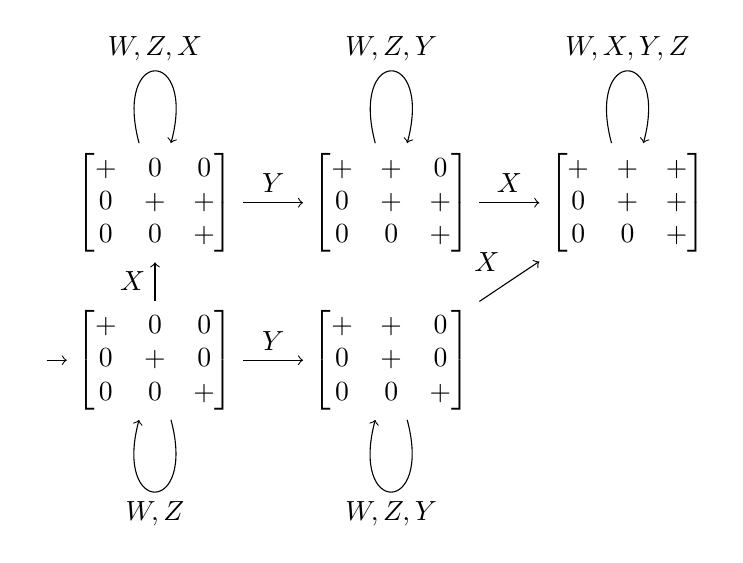
\begin{tikzpicture}
    \node(start) at (-1.5,0) {};
    \node(id) at (0,0) {$\begin{bmatrix}+&0&0\\0&+&0\\0&0&+\end{bmatrix}$};
    \node(cp) at (0,2) {$\begin{bmatrix}+&0&0\\0&+&+\\0&0&+\end{bmatrix}$};
    \node(acp) at (3,2) {$\begin{bmatrix}+&+&0\\0&+&+\\0&0&+\end{bmatrix}$};
    \node(ap) at (3,0) {$\begin{bmatrix}+&+&0\\0&+&0\\0&0&+\end{bmatrix}$};
    \node(abcp) at (6,2) {$\begin{bmatrix}+&+&+\\0&+&+\\0&0&+\end{bmatrix}$};
    \draw[->] (start) -- (id);
    \draw[->] (id) to node[auto] {$X$} (cp);
    \draw[->] (id) to node[auto] {$Y$} (ap);
    \draw[->] (cp) to node[auto] {$Y$} (acp);
    \draw[->] (acp) to node[auto] {$X$} (abcp);
    \draw[->] (ap) to node[auto] {$X$} (abcp);
    \draw[->,loop below] (id) to node[auto] {$W,Z$} (id);
    \draw[->,loop below] (ap) to node[auto] {$W,Z,Y$} (ap);
    \draw[->,loop above] (cp) to node[auto] {$W,Z,X$} (cp);
    \draw[->,loop above] (acp) to node[auto] {$W,Z,Y$} (acp);
    \draw[->,loop above] (abcp) to node[auto] {$W,X,Y,Z$} (abcp);
\end{tikzpicture}
\end{center}
Starting from the identity and applying the different products $e^{A_it_i}$ in the diagram,
it is clear that the only way to reach a matrix of the shape of $G$ is to have all
the ``$X$'' before ``$Y$''. Formally, by contradiction, if there were $i<j$ such
that $A_i=Y$ and $A_j=X$ then by the diagram, we would end up with a matrix where
the top right corner in nonzero, which is absurd.
\end{proof}

The previous lemma shows that this semigroup enforces a partial order on the matrices
in products that reach the matrix $G$. The next lemma shows that $G$ can indeed be reached using this
kind of products, essentially proving that $G$ belongs to this semigroup.

\begin{proposition}\label{prop:forced_order_exists}
For any $t>0$, there exists $u\geqslant0$ such that:
\[e^{Wu}e^{Xt}e^{Yt}e^{Zu}=G\quad\text{ or }\quad e^{Zu}e^{Xt}e^{Yt}e^{Wu}=G.\]
\end{proposition}

\begin{proof}
Consider the following products for an arbitrary $u\geqslant0$:
\begin{align*}
e^{Wu}e^{Xt}e^{Yt}e^{Zu}&=\begin{bmatrix}1&0&0\\0&e^u&0\\0&0&e^{2u}\end{bmatrix}
    \begin{bmatrix}1&t&0\\0&1&t\\0&0&1\end{bmatrix}
    \begin{bmatrix}1&0&0\\0&e^{-u}&0\\0&0&e^{-2u}\end{bmatrix}\\
&=\begin{bmatrix}1&0&0\\0&e^u&0\\0&0&e^{2u}\end{bmatrix}
    \begin{bmatrix}1&te^{-u}&0\\0&e^{-u}&te^{-2u}\\0&0&e^{-2u}\end{bmatrix}\\
&=\begin{bmatrix}1&te^{-u}&0\\0&1&te^{-u}\\0&0&1\end{bmatrix},
\end{align*}
and
\[
e^{Zu}e^{Xt}e^{Yt}e^{Wu}=\begin{bmatrix}1&te^{u}&0\\0&1&te^{u}\\0&0&1\end{bmatrix}.
\]
If $t\geqslant1$ then choosing $u=\ln t\geqslant0$ in the first product gives $G$,
otherwise choosing $u=\ln\frac{1}{t}\geqslant0$ in the second product gives $G$.
\end{proof}

\subsection{Undecidability of the semigroup problem}

We consider the following natural variant of MEP where the order of the matrices
in the product is not fixed and matrices can be used more than once.

\begin{definition}
  An instance of the Matrix-Exponential Semigroup Problem (MESP) consists of
  square matrices $A_{1}, \ldots, A_{k}$ and $C$, all of the same
  dimension, whose entries are real algebraic numbers.  The problem
 asks to determine whether $C$ a member of the matrix semigroup generated by
\begin{align*}
\lbrace \exp(A_{i} t_{i}) : t_{i} \geq 0 , i=1,\ldots,k \rbrace.
\end{align*}
\end{definition}

In the case where the matrices commute, MESP is equivalent to MEP. Will show that
if the matrices do not commute, this problem is undecidable by reducing from MEP,
which is undecidable in the non-commuting case.

\begin{theorem}
  MESP is undecidable in the non-commutative case.
\end{theorem}

\begin{proof}
We have seen in the previous section that MEP is undecidable in the non-commutative
case. Thus it suffices to reduce MEP to MESP to show undecidability.

Let $A_1,\ldots,A_k,C\in\Algebraics^{n\times n}$ be an instance of MEP. Denote by $I_m$ the identity of size $m$,
$0_m$ the zero matrix of size $m$. Recall that $W,X,Y,Z$ and $G$ were defined in the previous
subsection. For every $i\in\{2,\ldots,k-1\}$, define the following matrices:
\begin{align*}
B_i&=\begin{bmatrix}A_i&&&&\\&0_{3(i-2)}&&&\\&&Y&&\\&&&X&\\&&&&0_{3(k-1-i)}\end{bmatrix},\\
B_i'&=\begin{bmatrix}0_p&&&&\\&0_{3(i-2)}&&&\\&&Y&&\\&&&X&\\&&&&0_{3(k-1-i)}\end{bmatrix}.\\
\end{align*}
Also define the following matrices:
\[
\begin{array}{r@{}c@{}cr@{}c}
B_1=&\begin{bmatrix}A_1&&\\&X&\\&&0_{3(k-2)}\end{bmatrix},&&
B_1'=&\begin{bmatrix}0_p&&\\&X&\\&&0_{3(k-2)}\end{bmatrix},\\
B_k=&\begin{bmatrix}A_1&&\\&0_{3(k-2)}&\\&&Y\end{bmatrix},&&
B_k'=&\begin{bmatrix}0_p&&\\&0_{3(k-2)}&\\&&Y\end{bmatrix}.\\
\end{array}\]
Also define for every $i\in\{1,\ldots,k-1\}$:
\begin{align*}
W_i&=\begin{bmatrix}0_p&&&\\&0_{3(i-1)}&&\\&&W&\\&&&0_{3(k-1-i)}\end{bmatrix},\\
Z_i&=\begin{bmatrix}0_p&&&\\&0_{3(i-1)}&&\\&&Z&\\&&&0_{3(k-1-i)}\end{bmatrix}.\\
\end{align*}
And finally define the target matrix:
\[C'=\begin{bmatrix}C&&&\\&G&&\\&&\ddots&\\&&&G\end{bmatrix}.\]
We can now define our MESP instance as follows, the target matrix is $C'$ and the semigroup $\mathcal{G}$
is generated by:
\begin{align*}
&\left\{e^{B_it_i},e^{B_i't_i}:t_i\geqslant0,i=1,\ldots,k\right\}\\
&\cup\left\{e^{W_it_i},e^{Z_it_i}:t_i\geqslant0,i=1,\ldots,k-1\right\}.
\end{align*}
We claim the original instance of MEP is satisfiable if and only if $C'\in\mathcal{G}$.
Let us examine both direction independently.

Assume that the MEP instance is satisfiable. Then there exists $t_1,\ldots,t_k\geqslant0$ such that:
\[\prod_{i=1}^ke^{A_it_i}=C.\]
Define $\tau=\max\{t_1,\ldots,t_k\}+1$ (note that $\tau>0$) and $t_i'=\tau-t_i\geqslant0$ for every $i\in\{1,\ldots,k\}$.
A straightforward calculation shows that:
\begin{align*}
\prod_{i=1}^k\left(e^{B_it_i}e^{B_i't_i'}\right)
    &=\begin{bmatrix}\prod_{i=1}^ke^{A_it_i}&&&\\&e^{X\tau}e^{Y\tau}&&\\&&\ddots&\\&&&e^{X\tau}e^{Y\tau}\end{bmatrix}\\
    &=\begin{bmatrix}C&&&\\&U&&\\&&\ddots&\\&&&U\end{bmatrix},
\end{align*}
where $U=e^{X\tau}e^{Y\tau}$. Apply \cref{prop:forced_order_exists} to get $\lambda\geqslant0$
such that either $e^{W\lambda}Ue^{Z\lambda}=G$ or $e^{Z\lambda}Ue^{W\lambda}=G$. In the first case, conclude by
checking that:
\[
\prod_{i=1}^{k-1}e^{W_i\lambda}\prod_{i=1}^k\left(e^{B_it_i}e^{B_i't_i'}\right)\prod_{i=1}^{k-1}e^{Z_i\lambda}
    =\begin{bmatrix}C&&&\\&G&&\\&&\ddots&\\&&&G\end{bmatrix}=C'
\]
In the second case, exchange the $W_i$ and $Z_i$ to get same result. This concludes the proof that
the MESP instance is satisfiable, since all the products belong to $\mathcal{G}$.

Assume that the MESP instance is satisfiable. Then there exists $t_1,\ldots,t_m>0$ (we can always take them positive)
and $M_1,\ldots,M_m\in\big\{B_i,B_i':i=1,\ldots,k\}\cup\big\{W_i,Z_i:i=1,\ldots,k-1\big\}$
such that:
\begin{equation}\label{eq:mesp_to_mep:prod_eq}
\prod_{j=1}^me^{M_jt_j}=C'.
\end{equation}
Observe that by construction, this product has the following form:
\[\prod_{j=1}^me^{M_jt_j}=\begin{bmatrix}V&&&\\&U_1&&\\&&\ddots&\\&&&U_{k-1}\end{bmatrix},\]
where $V$ belongs to the semigroup generated by $\{e^{A_it}:t\geqslant0\}$ and $U_i$ belongs
to the semigroup generated by $\{e^{Wt},e^{Xt},e^{Yt},e^{Zt}:t\geqslant0\}$. Since
\eqref{eq:mesp_to_mep:prod_eq} implies that $U_i=G$, we can apply \cref{prop:eq_has_forced_order}
to get each product producing $U_i$ must have all its ``$X$'' before its ``$Y$''. Furthermore, each $U_i$
must contain at least one $X$ and one $Y$ in its product. For any $i\in\{1,\ldots,k\}$,
let $k_i$ (resp. $k_i'$) denote
the first (resp. last) index $j$ such that $M_j=B_i\text{ or }B_i'$. Those indices exists because
of the proposition since at least one $B_i$ or $B_i$' must appear for every $i$
to get both an $X$ and a $Y$ in each product giving $U_i$. Obviously $k_i\leqslant k_i'$
by definition. We now claim that the proposition implies that:
\[k_1\leqslant k_1'<k_2\leqslant k_2'<k_3\cdots<k_{k-1}\leqslant k_{k-1}'.\]
Indeed, \cref{prop:eq_has_forced_order} ensures that in the product giving $U_1$,
all the ``$X$'' appear before the ``$Y$'',
but the only matrices that contribute some $X$ to $U_1$ are $B_1$ and $B_1'$,
and the only matrices that contribute some $Y$ to $U_1$ are $B_2$ and $B_2'$.
Thus $k_1'<k_2$, \emph{i.e.} the last ``$X$'' coming from $B_1$ or $B_1'$ is before the first ``$Y$''
coming from $B_2$ or $B_2'$. A similar reasoning ensures that $k_2'<k_3$ and so on.
This shows that for any $i\in\{1,\ldots,k\}$, if $M_j=B_i$ then $j\in\{k_i,\ldots,k_i'\}$. Thus all
the $B_1$ appear before the $B_2$ which appear before the $B_3$ and so on.
But since the $B_i$ are the only one to contribute to $V$, $V$ must be of the form:
\[V=\prod_{i=1}^ke^{A_it_i'},\]
where $t_i'\geqslant0$ is the sum of all $t_j$ such that $M_j=B_i$.
Finally $V=C$, so the instance of MEP is satisfiable.

\end{proof}
\section{Other Undecidability Results}

Consider the following generalisation of the Continuous Orbit Problem: given $k$ matrices $A_{1}, \ldots, A_{k} \in \Algebraics^{n \times n}$ and two vectors $\myvector{x}, \myvector{y} \in \Algebraics^{n}$, all with real coordinates, do there exist $t_{1}, \ldots, t_{k} \geq 0$ such that
\begin{equation}
\prod \limits_{i=1}^{k} \exp(A_{i} t_{i}) \myvector{x} = \myvector{y} ?
\end{equation}

\begin{theorem}
The Generalised Continuous Orbit Problem is undecidable.
\end{theorem}

\begin{proof}
This can be shown by reduction from MEP. Suppose we are trying to decide whether there exist $t_{1}, \ldots, t_{k}$ such that
\begin{equation*}
\prod \limits_{i=1}^{k} \exp(B_{i} t_{i}) = C .
\end{equation*}
Let $\myvector{c}_{1}, \ldots, \myvector{c}_{n}$ be the columns of $C$, from left to right, and let $\myvector{e}_{1}, \ldots, \myvector{e}_{n}$ denote the canonical basis of $\Reals^{n}$. For each $i \in \lbrace 1, \ldots, n \rbrace$, we define
\begin{equation*}
A_{i} =
\begin{pmatrix}
B_{i} && \cdots && 0 \\
\vdots && \ddots && \vdots \\
0 && \cdots && B_{i}
\end{pmatrix}
\end{equation*}
Then
\begin{equation*}
\prod \limits_{i=1}^{k} \exp(B_{i} t_{i}) = C \Leftrightarrow \prod \limits_{i=1}^{k} \exp(A_{i} t_{i}) \begin{pmatrix} \myvector{e}_{1} \\ \vdots \\ \myvector{e}_{n} \end{pmatrix} = \begin{pmatrix} \myvector{c}_{1} \\ \vdots \\ \myvector{c}_{n} \end{pmatrix} .
\end{equation*}
\end{proof}

Moreover, consider the following generalisation of the Continuous Skolem Problem: given $k$ matrices $A_{1}, \ldots, A_{k} \in \Algebraics^{n \times n}$ and two vectors $\myvector{x}, \myvector{y} \in \Algebraics^{n}$, all with real coordinates, do there exist $t_{1}, \ldots, t_{k} \geq 0$ such that
\begin{equation}
\myvector{x}^{T} \prod \limits_{i=1}^{k} \exp(A_{i} t_{i}) \myvector{y} = 0 ?
\end{equation}

\begin{theorem}
The Generalised Continuous Skolem Problem is undecidable.
\end{theorem}

\begin{proof}
This can be shown by reduction from the Generalised Continuous Orbit Problem. Suppose we are trying to decide whether there exist $t_{1}, \ldots, t_{k}$ such that
\begin{equation*}
\prod \limits_{i=1}^{k} \exp(A_{i} t_{i}) \myvector{x} = \myvector{y} .
\end{equation*}
Let $\myvector{e}_{1}, \ldots, \myvector{e}_{n}$ denote the canonical basis of $\Reals^{n}$. Moreover, let
\begin{equation*}
B_{i} = \begin{pmatrix} A_{i} && 0 \\ 0 && 0 \end{pmatrix},
\myvector{u}_{j} = \begin{pmatrix} \myvector{e}_{j} \\ - \myvector{e}_{j} \end{pmatrix},
\myvector{v} = \begin{pmatrix} \myvector{x} \\ \myvector{y} \end{pmatrix} .
\end{equation*}
Moreover, let
\begin{equation*}
C_{i} = \begin{pmatrix} B_{i} \otimes I + I \otimes B_{i} && \cdots && 0 \\ \vdots && \ddots && \vdots \\ 0 && \cdots && B_{i} \otimes I + I \otimes B_{i} \end{pmatrix} .
\end{equation*}
Then
\begin{align*}
&\prod \limits_{i=1}^{k} \exp(A_{i} t_{i}) \myvector{x} = \myvector{y} \\
\Leftrightarrow &\sum \limits_{j=1}^{n} \left( \myvector{u}_{j}^{T} \prod \limits_{i=1}^{k} \exp(B_{i} t_{i}) \myvector{v} \right)^{2} = 0 \\
\Leftrightarrow &\sum \limits_{j=1}^{n} \left( \left( \myvector{u}_{j} \otimes \myvector{u}_{j} \right) \prod \limits_{i=1}^{k} \left( \exp( B_{i} t_{i} ) \otimes \exp(B_{i} t_{i}) \right) \left( \myvector{v} \otimes \myvector{v} \right) \right) = 0 \\
\Leftrightarrow &\sum \limits_{j=1}^{n} \left( \left( \myvector{u}_{j} \otimes \myvector{u}_{j} \right) \prod \limits_{i=1}^{k} \exp\left((B_{i} \otimes I + I \otimes B_{i}) t_{i} \right) \left( \myvector{v} \otimes \myvector{v} \right) \right) = 0 \\
\Leftrightarrow &\begin{pmatrix} \myvector{u}_{1} \otimes \myvector{u}_{1} \\ \vdots \\ \myvector{u}_{n} \otimes \myvector{u}_{n} \end{pmatrix} \prod \limits_{i=1}^{k} \exp( C_{i} t_{i} ) \begin{pmatrix} \myvector{v} \otimes \myvector{v} \\ \vdots \\ \myvector{v} \otimes \myvector{v} \end{pmatrix} = 0 .
\end{align*}
\end{proof}

\chapter{The Polytope Escape Problem}
\section{Introduction}

In ambient space $\Reals^{d}$, a \emph{continuous linear
  dynamical system} is a trajectory $\myvector{x}(t)$, where $t$
ranges over the non-negative reals, defined by a differential equation
$\dot{\myvector{x}}(t)=f(\myvector{x}(t))$ in which the function
$f$ is \emph{affine} or \emph{linear}. If the initial point
$\myvector{x}(0)$ is given, the differential equation uniquely
defines the entire trajectory. (Linear) dynamical systems have been
extensively studied in Mathematics, Physics, and Engineering, and more
recently have played an increasingly important role in Computer
Science, notably in the modelling and analysis of cyber-physical
systems; a recent and authoritative textbook on the matter
is~\cite{Alu15}.

In the study of dynamical systems, particularly from the perspective
of control theory, considerable attention has been given to the study
of \emph{invariant sets}, i.e., subsets of $\Reals^{d}$ from which
no trajectory can escape; see, e.g.,
\cite{CastelanH92,BlondelT00,BM07,SDI08}. Our focus in the present
chapter is on sets with the dual property that \emph{no trajectory
  remains trapped}. Such sets play a key role in analysing
\emph{liveness} properties in cyber-physical systems (see, for
instance,~\cite{Alu15}): discrete progress is ensured by
guaranteeing that all trajectories (i.e., from any initial starting
point) must eventually reach a point at which they `escape'
(temporarily or permanently) the set in question.

More precisely, given an affine function
$f:\Reals^{d}\rightarrow \Reals^{d}$ and a convex polytope
$\mathcal{P}\subseteq\Reals^{d}$, both specified using rational
coefficients encoded in binary, we consider the \emph{Polytope
  Escape Problem} which asks whether there is some point
$\myvector{x}_0$ in $\mathcal{P}$ for which the corresponding
trajectory of the solution to the differential equation
\begin{equation*}
\begin{displaystyle} \begin{cases}
\dot{\myvector{x}}(t)=f(\myvector{x}(t)) \\
\myvector{x}(0)=\myvector{x}_{0}
\end{cases} \end{displaystyle}
\end{equation*}
is entirely contained in $\mathcal{P}$. Our main result is to show
that this problem is decidable by reducing it in polynomial time to
the decision version of linear programming with real algebraic
coefficients, which itself reduces in polynomial time to deciding the
truth of a sentence in the first-order theory of the reals, a problem
whose complexity is known to lie between $\NP$ and
$\PSPACE$ \cite{Canny88}. Our algorithm makes use of spectral
techniques and relies among others on tools from Diophantine
approximation.

It is interesting to note that a seemingly closely related problem,
that of determining whether a given trajectory of a linear dynamical
system ever hits a given hyperplane (also known as the
\emph{continuous Skolem Problem}), is not known to be decidable; see,
in particular,~\cite{ContinuousSkolem,ContinuousSkolem3,COW16b:LICS16}. When the
target is instead taken to be a single point (rather than a
hyperplane), the corresponding reachability question (known as the
\emph{continuous Orbit Problem}) can be decided in polynomial
time~\cite{Hainry08}.

\section{The Polytope Escape Problem}

The Polytope Escape Problem for continuous linear dynamical systems
consists of deciding, given an affine function
$f:\Reals^{d}\rightarrow \Reals^{d}$ and a convex polytope
$\mathcal{P}\subseteq\Reals^{d}$, whether there exists an initial point
$\myvector{x}_{0} \in \mathcal{P}$ for which the trajectory of the unique
solution to the differential equation
$\dot{\myvector{x}}(t)=f(\myvector{x}(t)),\myvector{x}(0)=\myvector{x}_{0},
t\geq 0$,
is entirely contained in $\mathcal{P}$.  A starting point
$\myvector{x}_{0}\in\mathcal{P}$ is said to be \textbf{trapped} if
the trajectory of the corresponding solution is contained in $\mathcal{P}$,
and \textbf{eventually trapped} if the trajectory of the corresponding
solution contains a trapped point. Therefore, the Polytope Escape
Problem amounts to deciding whether a trapped point exists, which in
turn is equivalent to deciding whether an eventually trapped point exists.

The goal of this section is to prove the following result:

\begin{theorem}
  The Polytope Escape Problem is polynomial-time reducible to the
  decision version of linear programming with algebraic coefficients.
\end{theorem}

A $d$-dimensional instance of the Polytope Escape Problem is a pair
$(f,\mathcal{P})$, where $f:\Reals^{d}\rightarrow \Reals^{d}$
is an affine function and $\mathcal{P}\subseteq\Reals^{d}$ is a
convex polytope. In this formulation we assume that all numbers
involved in the definition of $f$ and $\mathcal{P}$ are
rational.\footnote{The assumption of rationality is required to
  justify some of our complexity claims (e.g., Jordan Canonical Forms
  are only known to be polynomial-time computable for matrices with
  rational coordinates). Nevertheless, our procedure remains valid in
  a more general setting, and in fact, the overall
  $\exists \Reals$ complexity of our algorithm would not be
  affected if one allowed real algebraic numbers when defining problem
  instances.}

An instance $(f,\mathcal{P})$ of the Polytope Escape Problem is said
to be \textbf{homogeneous} if $f$ is a linear function and
$\mathcal{P}$ is a convex polytope cone (in particular,
$\myvector{x}\in\mathcal{P},\alpha>0\Rightarrow \alpha\myvector{x}
\in\mathcal{P}$).
%Moreover, an homogeneous instance of the Polytope Escape Problem is said to be \textbf{real} if all eigenvalues of $f$ are real.

The restriction of the Polytope Escape Problem to homogeneous
instances is called the homogeneous Polytope Escape Problem.

\begin{lemma}
  The Polytope Escape Problem is polynomial-time reducible to the
  homogeneous Polytope Escape Problem.
\end{lemma}

\begin{proof}
  Let $(f,\mathcal{P})$ be an instance of the Polytope Escape
  Problem in $\Reals^{d}$, and write
\begin{equation*}
f(\myvector{x})=A\myvector{x}+\myvector{a}\mbox{ and } \mathcal{P}=\lbrace\myvector{x}\in\Reals^{d}: B_{1}\myvector{x}>\myvector{b}_{1} \wedge B_2\myvector{x}\geq \myvector{b}_{2}\rbrace \, .
\end{equation*}
Now define
\begin{align*}
& A'=\begin{pmatrix}A & \myvector{a}\\ \myvector{0}^T & 0\end{pmatrix},
B_{1}'=\begin{pmatrix}B_{1} & -\myvector{b}_{1} \\ \myvector{0}^T & 1\end{pmatrix},
B_{2}'=\begin{pmatrix}B_{2} & -\myvector{b}_{2} \end{pmatrix} \, ,\\
& \mathcal{P}'=
\left\lbrace
\begin{pmatrix}\myvector{x}\\y
\end{pmatrix} \in\Reals^{d+1}:B_{1}'\begin{pmatrix}\myvector{x}\\y
\end{pmatrix}
  > \myvector{0}
  \wedge B_{2}'\begin{pmatrix}\myvector{x}\\y
\end{pmatrix} \geq \myvector{0} \right\rbrace \, ,
\intertext{and}
& g\begin{pmatrix}\myvector{x}\\y
\end{pmatrix} = A'\begin{pmatrix}\myvector{x}\\y
\end{pmatrix} \, .
\end{align*}
Then $(g,\mathcal{P}')$ is a homogeneous instance
of the Polytope Escape Problem.

It is clear that $\myvector{x}(t)$ satisfies the differential equation
$\dot{\myvector{x}}(t)=f(\myvector{x}(t))$ if and only if
$\begin{pmatrix}
\myvector{x}(t)\\1 \end{pmatrix}$ satisfies
the differential equation
$\begin{pmatrix}\dot{\myvector{x}}\\
\dot{y}
\end{pmatrix} = g\begin{pmatrix}\myvector{x}\\y
\end{pmatrix}$.  In general,
in any trajectory $\begin{pmatrix}\myvector{x}\\y
\end{pmatrix}$ that satisfies this last differential equation, the
$y$-component must be constant.

We claim that $(f,\mathcal{P})$ is a positive instance
of the Polytope Escape Problem if and
only if $(g,\mathcal{P}')$ is a positive instance.
Indeed, if the point
$\myvector{x}_0 \in \Reals^{d}$ is trapped
in $(f,\mathcal{P})$
then the point $\begin{pmatrix}\myvector{x}_0\\1
\end{pmatrix}$ is trapped in $(g,\mathcal{P}')$.
Conversely, suppose that $\begin{pmatrix}\myvector{x}_0\\y_0
\end{pmatrix}$ is trapped in  $(g,\mathcal{P}')$.  Then,
since $B_{1}'\begin{pmatrix}\myvector{x}_0\\y_0
\end{pmatrix}
> \myvector{0}$,
we must have $y_0>0$.  Scaling, it follows that
$\begin{pmatrix} y_0^{-1}\myvector{x}_0\\1
\end{pmatrix}$ is also trapped in $(g,\mathcal{P}')$.  This implies
that $y_0^{-1}\myvector{x}_0$ is trapped in $(f,\mathcal{P})$.
%
%In fact, if $\myvector{x}_{0}$ is
%a trapped point for $(f,\mathcal{P})$, then $(\myvector{x}_{0},1)$
%will be a trapped point for $(A',\mathcal{P}')$. Conversely, if
%$(\myvector{x}_{0},c)$ is a trapped point for $(A',\mathcal{P}')$,
%then $c^{-1}\myvector{x}_{0}$ is a trapped point for
%$(f,\mathcal{P})$. Note that $c>0$ must hold.
\end{proof}

We remind the reader that the unique solution to the differential equation $\dot{\myvector{x}}(t)=f(\myvector{x}(t)),\myvector{x}(0)=\myvector{x}_{0},t\geq 0$, where $f(\myvector{x})=A\myvector{x}$, is given by
$\myvector{x}(t)=\exp(At)\myvector{x}_{0}$.

In this setting, the sets of trapped and eventually trapped points are, respectively:
\begin{align*}
\mathit{T}&=\lbrace \myvector{x}_0\in\Reals^{d}: \forall t\geq 0, \exp(At)\myvector{x}_{0} \in \mathcal{P}\rbrace \\
\mathit{ET}&=\lbrace\myvector{x}_{0}\in\Reals^{d}:\exists t\geq 0,\exp(At)\myvector{x}_{0}\in\mathit{T}\rbrace
\end{align*}

Note that both $\mathit{T}$ and $\mathit{ET}$ are convex subsets of $\Reals^{d}$.

\begin{lemma}
  The homogeneous Polytope Escape Problem is polynomial-time
  reducible to the decision version of linear programming with
  algebraic coefficients.
\end{lemma}

\begin{proof}
  % Given an homogeneous instance of the Polytope Escape Problem
  % $(A,\mathcal{P})$, we can create an equivalent real homogeneous
  % instance of the Polytope Escape Problem $(A',\mathcal{P}')$ by
  % picking a basis
  % $\mathcal{B}=\lbrace \myvector{u}_{1},\ldots,\myvector{u}_{k}
  % \rbrace$
  % of $\mathcal{V}^{r}$ and taking $A'$ to be the matrix
  % representation of $A\vert_{\mathcal{V}^{r}}$ with respect to
  % $\mathcal{B}$ and
%\begin{align*}
%\mathcal{P}'=\lbrace\myvector{x}\in \Reals^{k} : \sum\limits_{i=1}^{k} x_{i}\myvector{u}_{i}\in\mathcal{P}\rbrace
%\end{align*}
%which is still a cone.

  Let
  $\myvector{x}_{0}=\myvector{x}_{0}^{r}+\myvector{x}_{0}^{c}$,
  where $\myvector{x}_{0}^{r}\in \mathcal{V}^{r}$ and
  $\myvector{x}_{0}^{c}\in \mathcal{V}^{c}$. We start by showing
  that if $\myvector{x}_{0}$ lies in the set $T$ of trapped points
  then its component $\myvector{x}_{0}^{r}$ in the real eigenspace
  $\mathcal{V}^{r}$ lies in the set $\mathit{ET}$ of eventually
  trapped points.
Due to the
fact that the intersection of finitely many convex polytopes is still
a convex polytope, it suffices to prove this claim for the case when
  $\mathcal{P}$ is defined by a single inequality---say
  $\mathcal{P}=\lbrace \myvector{x}\in\Reals^{d}:
  \myvector{b}^{T}\myvector{x}\triangleright 0\rbrace$, where
  $\triangleright$ is either $>$ or $\geq$.

  We may assume that
  $\myvector{b}^{T} \exp(At) \myvector{x}_{0}^{c}$ is not identically
  zero, as in that case
  $\myvector{b}^{T} \exp(At)\myvector{x}_{0} \equiv
  \myvector{b}^{T} \exp(At)\myvector{x}_{0}^{r}$ and our claim
  holds trivially.
  Also, if $\myvector{x}_{0}\in\mathit{T}$, it cannot hold that
  $\myvector{b}^{T} \exp(At) \myvector{x}_{0}^{r} \equiv 0$, since
  $\myvector{b}^{T} \exp(At) \myvector{x}_{0}^{c}$ is negative
  infinitely often by \cref{cor:liminf}.

  Suppose that $\myvector{x}_{0}\in\mathit{T}$ and let $(\rho,m)$
  and $(\eta,j)$ be the dominant indices for
  $\myvector{b}^{T} \exp(At) \myvector{x}_{0}^{r}$ and
  $\myvector{b}^{T} \exp(At) \myvector{x}_{0}^{c}$ respectively.
Then by \cref{prop:linear} we have
\begin{gather}
\myvector{b}^{T} \exp(At) \myvector{x}_{0}^{r} = \exp(\rho t)t^m (c
  + o(1))
\label{eq:real}
\end{gather}
 as $t \rightarrow \infty$, where $c$ is a non-zero real
number.  We will show that $c>0$, from which it follows  that
$\myvector{x}_{0}^{r} \in \mathit{ET}$.

%From this it follows that
%\begin{equation*}
%c=\lim\limits_{t\rightarrow \infty}
%\frac{\myvector{b}^{T}\exp(At)\myvector{x}_{0}^{r}}{\exp(\rho t)
%  t^{m}} \, .
%\end{equation*}
% From the fact that $(\rho,m)$ is dominant for
% $\myvector{b}^{T} \exp(At) \myvector{x}_{0}^{r}$, it follows that
% $\myvector{b}^{T} \exp(At) \myvector{x}_{0}^{r}

% $c$ is the coefficient of the term $t^me^{\rho t}$ in
% $\myvector{b}^{T} \exp(At) \myvector{x}_{0}^{r}$, and is therefore
% non-zero.

It must hold that $(\eta,j)\preceq (\rho,m)$.  Indeed, if $(\eta,j)\succ
(\rho,m)$, then, as $t\rightarrow\infty$,
\begin{align*}
\myvector{b}^{T} \exp(At) \myvector{x}_{0} = \exp(\eta t)t^{j} \Bigg(
\underbrace{\frac{\myvector{b}^{T} \exp(At) \myvector{x}_{0}^{c}}{\exp(\eta t)t^{j}}}_{\mytag{termA}} + o(1)\Bigg) ,
\end{align*}
%
but the limit inferior of the term~\ref{termA} above is strictly
negative by \cref{cor:liminf},
contradicting the fact that $\myvector{x}_{0}\in\mathit{T}$.

If $(\eta,j)=(\rho,m)$, then, as $t\rightarrow\infty$,
\begin{align*}
\myvector{b}^{T} \exp(At) \myvector{x}_{0} = \exp(\rho t)t^{m} \left( c + \frac{\myvector{b}^{T} \exp(At) \myvector{x}_{0}^{c}}{\exp(\rho t)t^{m}} + o(1) \right) ,
\end{align*}
and by invoking \cref{cor:liminf} as above, it follows that
$c > 0$.

% from which we conclude that
% $\myvector{x}_{0}^{r}\in\mathit{ET}$, since, as
% $t\rightarrow\infty$,
% \begin{align*}
% \myvector{b}^{T} \exp(At) \myvector{x}_{0}^{r} = \exp(\rho t)t^{m}
%   \left( c +o(1) \right) \, .
% \end{align*}
Finally, if $(\eta,j)\prec (\rho,m)$, then, as $t\rightarrow\infty$,
\begin{gather}\myvector{b}^{T} \exp(At) \myvector{x}_{0}^c =
\exp(\rho t)t^{m} \cdot o(1) \, ,
\label{eq:complex}
\end{gather} and hence, by (\ref{eq:real}) and (\ref{eq:complex}), it
follows that
\begin{align*}
\myvector{b}^{T} \exp(At) \myvector{x}_{0} = \exp(\rho t)t^{m} \left( c +o(1) \right) \, .
\end{align*}
From the fact that $\myvector{x}_{0} \in T$ and that $c\neq 0$ we must have $c>0$.

In all cases it holds that $c>0$ and hence
$\myvector{x}_{0}^{r}\in\mathit{ET}$.


%\end{proof}
%\begin{lemma}
%The restriction of the Polytope Escape Problem to real homogeneous instances is decidable in polynomial time.
%\end{lemma}
%\begin{proof}

%  Suppose we are given a real homogeneous instance of the Polytope
%  Escape Problem $(A,\mathcal{P})$. We claim that, in this setting,
%  the set $\mathit{ET}$ is a convex polytope that we can
%  efficiently compute.



Having argued that
$\mathit{ET}\neq\emptyset$ iff $\mathit{ET}\cap
\mathcal{V}^{r}\neq\emptyset$,
we will now show that the set $\mathit{ET}\cap \mathcal{V}^{r}$ is a
convex polytope that we can efficiently compute. As before, it
suffices to prove this claim for the case when
$\mathcal{P}=\lbrace \myvector{x}\in\Reals^{d}:
\myvector{b}^{T}\myvector{x}\triangleright 0\rbrace$
(where $\triangleright$ is either $>$ or $\geq$).

In what follows, we let $[K]$ denote the set $\lbrace 0,\ldots,K-1 \rbrace$. We can write
\begin{align*}
\myvector{b}^{T}\exp(At)=\sum\limits_{(\eta,j)\in\sigma(A)\times
  [\nu(A)]} \exp(\eta t)t^{j} \myvector{u}_{(\eta,j)}^{T} \, ,
\end{align*}
where $\myvector{u}_{(\eta,j)}^{T}$ is the vector of coefficients of
$t^j\exp(\eta t)$ in $\myvector{b}^{T}\exp(At)$.

Note that if $\myvector{x}\in\mathcal{V}^{r}$ and $(\eta,j)\in
(\sigma(A)\setminus \Reals)\times \Naturals_{0}$, then
$\myvector{u}_{(\eta,j)}^{T}\myvector{x}=0$, as
$\myvector{u}_{(\eta,j)}^{T}\myvector{x}$ is the coefficient of $t^{j} \exp(\eta
t)$ in $\myvector{b}^{T}\exp(At) \myvector{x}$, and $\mathcal{V}^{r}$ is
invariant under $\exp(At)$. Moreover,
%
\begin{align*}
\mathit{ET}\cap\mathcal{V}^{r}=(\mathcal{B}\cap\mathcal{C}) \cup
\begin{cases}
\lbrace \myvector{0} \rbrace & \text{ if } \triangleright \text{ is } \geq \\
\emptyset & \text{ if } \triangleright \text{ is } >
\end{cases}
%\mathit{ET}\cap\mathcal{V}^{r}=(\mathcal{B}\cap\mathcal{C})\cup\lbrace \myvector{0}\mbox{ if }\triangleright\mbox{ is }\geq\mbox{ as opposed to }> \rbrace
\end{align*}
where
\begin{align*}
\mathcal{B}=&\bigcap\limits_{(\eta,j)\in (\sigma(A)\setminus \Reals)\times [\nu(A)]} \lbrace \myvector{x}\in\Reals^{d}: \myvector{u}_{(\eta,j)}^{T} \myvector{x}=0 \rbrace \\
\mathcal{C}=&\bigcup\limits_{(\eta,j)\in(\sigma(A)\cap \Reals)\times [\nu(A)]} \bigg[ \lbrace \myvector{x}\in\Reals^{d}: \myvector{u}_{(\eta,j)}^{T} \myvector{x}>0 \rbrace \cap \\
&\bigcap\limits_{(\rho,m)\succ (\eta,j)} \lbrace \myvector{x}\in\Reals^{d}: \myvector{u}_{(\rho,m)}^{T} \myvector{x}=0 \rbrace \bigg]
\end{align*}

The set $\mathit{ET}\cap\mathcal{V}^{r}$ can be seen to be convex from
the above characterisation. Alternatively, note that $\mathit{ET}$ can
be shown to be convex from its definition and that $\mathcal{V}^{r}$
is convex, therefore so must be their intersection. Thus
$\mathit{ET}\cap\mathcal{V}^{r}$ must be a convex polytope whose
definition possibly involves canonically-represented real algebraic
numbers, and the Polytope Escape Problem reduces to testing this
polytope for non-emptiness.
\end{proof}


\chapter{Reachability for Linear Time-Invariant Control Systems}
\section{Introduction}
In this chapter, we study a basic problem in control theory, namely the point-to-point controllability problem for both continuous- and discrete-time linear time-invariant (henceforth LTI) systems.

A discrete-time LTI system ${(\myvector{x}_{n})}_{n \in \Naturals} \subseteq \Reals^{d}$ with control set $\mathcal{U} \subseteq \Reals^{d}$ satisfies the evolution rule $\myvector{x}_{n+1} = A \myvector{x}_{n} + \myvector{u}_{n}$, where $A$ is a $d \times d$ matrix and $\myvector{u}_{n} \in \mathcal{U}$.
In words, the next state $\myvector{x}_{n+1}$ of the system is obtained by applying a time-invariant linear function to the previous state $\myvector{x}_{n}$ and adding a control $\myvector{u}_{n}$ from a time-invariant set $\mathcal{U}$ of controls.

Given two points $\myvector{s}, \myvector{t} \in \mathbb{R}^{d}$, the \emph{point-to-point controllability question for discrete-time LTI systems} consists in deciding whether there exist $n \in \Naturals$ and ${(\myvector{u}_{i})}_{i=0}^{n-1} \subseteq \mathcal{U}$ such that $\myvector{x}_{0} = \myvector{s}$ and $\myvector{x}_{n} = \myvector{t}$.

We show that this problem is undecidable when $\mathcal{U}$ is non-convex (in particular, when it is a finite union of convex polytopes) and that there is a reduction from Skolem's Problem when $\mathcal{U}$ is a convex polytope. This contrasts with the case where $\mathcal{U}$ is a linear subspace, in which case the problem reduces to the Orbit Problem, known to be decidable~\cite{Harrison}.

Similarly to the discrete case, a continuous-time LTI system $\myvector{x}(t) \subseteq \Reals^{d}$ with control set $\mathcal{U} \subseteq \Reals^{d}$ is a function satisfying the evolution rule $\dot{\myvector{x}}(t) = A \myvector{x}(t) + \myvector{u}(t)$
where $A$ is a $d \times d$ matrix and $\myvector{u}$ is a measurable function with codomain $\mathcal{U}$. The \emph{point-to-point controllability question for continuous-time LTI systems} consists in deciding whether there exist $t \geq 0$ and $\myvector{u} : [0,t] \rightarrow \mathcal{U}$ such that $\myvector{x}(0) = \myvector{s}$ and $\myvector{x}(t) = \myvector{t}$.

We show that this problem is in \PTIME{} when $\mathcal{U}$ is a linear subspace, by presenting a polynomial-time reduction to the Continuous Orbit Problem, which is known to be in \PTIME{}~\cite{ContinuousOrbitIPL}.

A survey of computational complexity results in control theory can be found in~\cite{BlondelT00}.

\section{Discrete-time systems}
\subsection{Hard Instances}

In this section, we present a hardness result for the point-to-point controllability problem for LTI systems where the set of admissible controls is a compact convex polytope.

We recall that Skolem's problem and the Positivity Problem are two long-standing open problems, whose decidability has not yet been determined.
It is known that the Positivity Problem is Skolem-hard~\cite{OW14:SODA}.
Instead of reducing from the Positivity Problem directly, we shall proceed by reducing from the following problem, which has been shown to be Positivity-hard in~\cite{MRP}:
\begin{definition}
Given a column-stochastic matrix $M \in \Rationals^{d \times d}$ and a number $r \in \Rationals \cap [0,1]$,
the \emph{Markov Reachability Problem} consists in determining whether there exists a number $n \in \Naturals$ such that ${\left( M^{n} \right)}_{1,2} \geq r$.
\end{definition}

We will now show the following result:

\begin{theorem}
The point-to-point controllability problem for LTI systems whose set of admissible controls are compact convex polytopes is Positivity-hard.
\end{theorem}

\begin{proof}
Given a column-stochastic matrix $M \in \mathbb{Q}^{d \times d}$ and a number $r \in \mathbb{Q} \cap [0,1]$, we define the matrix $A=\diag{M, 0, 0, 1} \in \mathbb{Q}^{(d+3)\times (d+3)}$ and the compact convex polytope
%Note: We want P to contain the origin, otherwise this could be simplified.
\begin{equation*}
\mathcal{P} = \lbrace (-\myvector{x}, y, \myvector{x} \cdot \myvector{1}, \myvector{x} \cdot \myvector{1}), \myvector{x} \geq \myvector{0}, \myvector{x} \cdot \myvector{1} \leq 1, 0 \leq y \leq \myvector{x} \cdot \myvector{e}_{1} \rbrace \subseteq \mathbb{R}^{d+3},
\end{equation*}
as well as the source $\myvector{s} = (\myvector{e}_{2}, 0, 0, 0) \in \mathbb{Q}^{d+3}$ and target $\myvector{t} = (\myvector{0}, r, 1, 1) \in \mathbb{Q}^{d+3}$.

First, suppose that there exists $n \in \mathbb{N}$ such that ${\left( M^{n} \right)}_{1,2} \geq r$. Consider the sequence of controls ${\left( \myvector{u}_{i} \right)}_{i=0}^{i=n-1} \subseteq \mathcal{P}$ given by $\myvector{u}_{0} = \cdots = \myvector{u_{n-2}} = \myvector{0}$ and $\myvector{u}_{n-1}$ is the element from $\mathcal{P}$ corresponding to $\myvector{x} = M^{n} \myvector{e}_{2}$ and $y=r$.
This sequence clearly controls $\myvector{s}$ to $\myvector{t}$.

On the other hand, suppose there exists a sequence ${\left( \myvector{u}_{i} \right)}_{i=0}^{i=n-1}$ controlling $\myvector{s}$ to $\myvector{t}$.
From the fact that the coordinates $d+2$ and $d+3$ of $\myvector{t}$ are equal, and noting that multiplying by the matrix $A$ erases coordinate $d+2$ but not $d+3$, it follows that $\myvector{u}_{n-1}$ is the only non-zero control, that is, $\myvector{u}_{0} = \cdots = \myvector{u}_{n-2} = \myvector{0}$.
Therefore, at time $n-1$, we will be in state $(M^{n-1} \myvector{e}_{2}, 0, 0, 0)$, and the only way to reach $\myvector{t}$ in the remaining step is to take $\myvector{u}_{n-1} \in \mathcal{P}$ with $\myvector{x} = M^{n} \myvector{e}_{2}$ and $y=r$, otherwise one of the first $d$ coordinates will be non-zero. It then follows that ${\left( M^{n} \right)}_{1,2} \geq r$, by looking at coordinate $d+1$.
\end{proof}

\section{Some undecidable matrix problems}

\label{matrix-undecidability}

Given $k+1$ invertible matrices $A_{1}, \ldots, A_{k},C \in \Rationals^{d \times d}$, the \emph{generalized matrix powering problem for invertible matrices} consists in deciding whether there exist $n_{1}, \ldots, n_{k} \in \Integers$ such that
\begin{equation*}
\prod\limits_{i=1}^{k} A_{i}^{n_{i}} = C.
\end{equation*}

\begin{theorem}
The generalized matrix powering problem for invertible matrices is undecidable.
\end{theorem}

\begin{proof}
We will show this result by reducing from Hilbert's Tenth Problem. Given a polynomial $p \in \Integers[n_{1}, \ldots, n_{k}]$, it is easy to express $p(n_{1}, \ldots, n_{k})$ as a conjunction of relations of the following form (noting that we may need to introduce new variables):
\begin{itemize}
\item $z = k$, where $k \in \Integers$
\item $z = x+y$
\item $z = xy$.
\end{itemize}
We start by showing how to encode each of these as an instance of the generalized matrix powering problem for invertible matrices.
Firstly, note that
\begin{equation*}
z = k \Leftrightarrow
\begin{pmatrix}
    1 & 1 \\
    0 & 1
\end{pmatrix}^{z} =
\begin{pmatrix}
    1 & k \\
    0 & 1
\end{pmatrix}.
\end{equation*}
Secondly, note that
\begin{equation*}
    z = x + y \Leftrightarrow
\begin{pmatrix}
    1 & 1 \\
    0 & 1
\end{pmatrix}^{x}
\begin{pmatrix}
    1 & 1 \\
    0 & 1
\end{pmatrix}^{y}
\begin{pmatrix}
    1 & -1 \\
    0 & 1
\end{pmatrix}^{z} =
\begin{pmatrix}
    1 & 0 \\
    0 & 1
\end{pmatrix}.
\end{equation*}
Thirdly, note that
\begin{equation*}
    z = xy \Leftrightarrow
    \exists x',y' \in \Integers,
    \begin{pmatrix}
        1 & 0 & 0 \\
        0 & 1 & 0 \\
        0 & 0 & 1
    \end{pmatrix} =
    \begin{pmatrix}
        1 & x-x' & z-xy \\
        0 & 1 & y-y' \\
        0 & 0 & 1
    \end{pmatrix}
\end{equation*}
and that the latter matrix is just equal to
\begin{equation*}
    \begin{pmatrix}
        1 & 0 & -1 \\
        0 & 1 & 0 \\
        0 & 0 & 1
    \end{pmatrix}^{z}
    \begin{pmatrix}
        1 & 0 & 0 \\
        0 & 1 & -1 \\
        0 & 0 & 1
    \end{pmatrix}^{y'}
    \begin{pmatrix}
        1 & 1 & 0 \\
        0 & 1 & 0 \\
        0 & 0 & 1
    \end{pmatrix}^{x}
    \begin{pmatrix}
        1 & 0 & 0 \\
        0 & 1 & 1 \\
        0 & 0 & 1
    \end{pmatrix}^{y}
    \begin{pmatrix}
        1 & -1 & 0 \\
        0 & 1 & 0 \\
        0 & 0 & 1
    \end{pmatrix}^{x'}.
\end{equation*}
Finally, conjunction can be achieved by making use of separate matrix blocks:
\begin{equation*}
    \prod\limits_{i=1}^{k} A_{i}^{n_{i}} = C \wedge \prod\limits_{i=1}^{k} B_{i}^{n_{i}} = D \Leftrightarrow
    \prod\limits_{i=1}^{k} \begin{pmatrix}A_{i} & 0 \\ 0 & B_{i}\end{pmatrix}^{n_{i}} = \begin{pmatrix}C & 0 \\ 0 & D\end{pmatrix}.
\end{equation*}
\end{proof}

\begin{definition}
Given invertible matrices $A_{1}, \ldots, A_{k} \in \Rationals^{d \times d}$ and two non-zero vectors $\myvector{x}, \myvector{y} \in \Rationals^{d}$, the \emph{vector reachability problem for invertible matrices} consists in deciding whether there exist $n_{1}, \ldots, n_{k} \in \Integers$ such that
\begin{equation*}
\prod\limits_{i=1}^{k}A_{i}^{n_{i}} \myvector{x} = \myvector{y}.
\end{equation*}
\end{definition}

\begin{theorem}
The vector reachability problem for invertible matrices is undecidable.
\end{theorem}

\begin{proof}
This can be shown by reduction from the generalised matrix powering problem for invertible matrices. In particular, given invertible matrices $A_{1}, \ldots, A_{k}, B \in \Rationals^{d \times d}$, letting $\myvector{b}_{1}, \ldots, \myvector{b}_{d}$ denote the columns of $B$, and letting $\myvector{e}_{1}, \ldots, \myvector{e}_{d}$ denote the canonical basis of $R^{d}$, the result follows from the fact that
    \begin{equation*}
        \prod\limits_{i=1}^{k} A_{i}^{n_{i}} = B \Leftrightarrow
        \prod\limits_{i=1}^{k}
        \begin{pmatrix}
            A_{i} & \cdots & 0 \\
            \vdots& \ddots & \vdots \\
            0 & \cdots & A_{i}
        \end{pmatrix}^{n_{i}}
        \begin{pmatrix}
            \myvector{e}_{1} \\
            \vdots \\
            \myvector{e}_{d}
        \end{pmatrix} =
        \begin{pmatrix}
            \myvector{b}_{1} \\
            \vdots \\
            \myvector{b}_{d}
        \end{pmatrix}.
    \end{equation*}
\end{proof}

\subsection{Undecidable instances}
\label{sec:lti_undecidability}

The goal of this section is to prove the following result.

\begin{theorem}
The point-to-point controllability problem for LTI systems whose sets of admissible controls are disjoint unions of finitely many closed convex polytopes is undecidable.
\end{theorem}

\begin{proof}
We prove this by reduction from the vector reachability problem for invertible matrices (defined in~\cref{sec:matrix-undecidability}).

Let $A_{1}, \ldots, A_{k} \in \Rationals^{d \times d}$ be invertible matrices and $\myvector{x}, \myvector{y} \in \Rationals^{d}$ be non-zero vectors.

For each $i \in \lbrace 1, \ldots, k \rbrace$, we define
\begin{equation*}
B_{i} =
\begin{pmatrix}
I_{d} & 0 & 0 \\
0 & A_{i} & 0 \\
0 & 0 & A_{i}^{-1} \\
\end{pmatrix}
\end{equation*}
and $M = \diag{B_{k}, \ldots, B_{1}, I_{d}, 1} \in \mathbb{Q}^{((3k+1)d+1) \times ((3k+1)d+1)}$.

Moreover, we let, for each $i \in \lbrace 1, \ldots, k \rbrace$,
\begin{align*}
\mathcal{P}_{i}^{(1)} &= {\lbrace \boldsymbol{0} \rbrace}^{3(k-i)d} &\times
\lbrace (-\boldsymbol{z}, \boldsymbol{z}, \boldsymbol{0}, \boldsymbol{0}), \boldsymbol{z} \in \mathbb{R}^{d} \rbrace &\times
{\lbrace \boldsymbol{0} \rbrace}^{3(i-1)d} &\times \lbrace 1 \rbrace
\subseteq \mathbb{R}^{(3k+1)d+1} \\
\mathcal{P}_{i}^{(2)} &= {\lbrace \boldsymbol{0} \rbrace}^{3(k-i)d} &\times
\lbrace (-\boldsymbol{z}, \boldsymbol{0}, \boldsymbol{z}, \boldsymbol{0}), \boldsymbol{z} \in \mathbb{R}^{d} \rbrace &\times
{\lbrace \boldsymbol{0} \rbrace}^{3(i-1)d} &\times \lbrace 1 \rbrace
\subseteq \mathbb{R}^{(3k+1)d+1} \\
\mathcal{Q}_{i}^{(1)} &= {\lbrace \boldsymbol{0} \rbrace}^{3(k-i)d} &\times
\lbrace (\boldsymbol{0}, -\boldsymbol{z}, \boldsymbol{0}, \boldsymbol{z}), \boldsymbol{z} \in \mathbb{R}^{d} \rbrace &\times
{\lbrace \boldsymbol{0} \rbrace}^{3(i-1)d} &\times \lbrace 1 \rbrace
\subseteq \mathbb{R}^{(3k+1)d+1} \\
\mathcal{Q}_{i}^{(2)} &= {\lbrace \boldsymbol{0} \rbrace}^{3(k-i)d} &\times
\lbrace (\boldsymbol{0}, \boldsymbol{0}, -\boldsymbol{z}, \boldsymbol{z}), \boldsymbol{z} \in \mathbb{R}^{d} \rbrace &\times
{\lbrace \boldsymbol{0} \rbrace}^{3(i-1)d} &\times \lbrace 1 \rbrace
\subseteq \mathbb{R}^{(3k+1)d+1}.
\end{align*}
We also let $\mathcal{P}_{1} = \mathcal{P}_{i}^{(1)} \dot{\cup} \mathcal{P}_{i}^{(2)}$ and $\mathcal{Q}_{1} = \mathcal{Q}_{i}^{(1)} \dot{\cup} \mathcal{Q}_{i}^{(2)}$.
We define the set of admissible controls as
\begin{align*}
\mathcal{U} = \bigcup\limits_{i=1}^{k} \left( \mathcal{P}_{i} \dot{\cup} \mathcal{Q}_{i} \right) \dot{\cup} \lbrace \boldsymbol{0} \rbrace.
\end{align*}
Finally, defining $\boldsymbol{s} = (\boldsymbol{x}, \boldsymbol{0}, \ldots, \boldsymbol{0}, 0)$, and $\boldsymbol{t} = (\boldsymbol{0}, \ldots, \boldsymbol{0}, \boldsymbol{y}, 2k)$, it holds that $\boldsymbol{s}$ can be controlled to $\boldsymbol{t}$ if and only if there exist $n_{1}, \ldots, n_{k} \in \mathbb{Z} \setminus \lbrace 0 \rbrace$ such that
\begin{equation*}
\prod\limits_{i=1}^{k}A_{i}^{n_{i}} \boldsymbol{x} = \boldsymbol{y}.
\end{equation*}

For one implication, suppose that such $n_{1}, \ldots, n_{k}$ exist.
We can use precisely $2k$ non-zero controls, which will correspond to times
$t_{1} = 0,
t_{2} = \lvert n_{1}\rvert,
t_{3} = \lvert n_{1} \rvert +1,
\ldots,
t_{2k-1} = \lvert n_{1} \rvert + \cdots + \lvert n_{k-1} \rvert + k-1,
t_{2k} = \lvert n_{1} \rvert + \cdots + \lvert n_{k} \rvert + k-1$.
For each $i \in \lbrace 0, \ldots, k-1 \rbrace$, $\myvector{u}_{t_{2i+1}}$ will belong $\mathcal{P}_{k-i}^{(1)}$ or $\mathcal{P}_{k-i}^{(2)}$ when $n_{k-i} \geq 0$ and $n_{k-i} < 0$ respectively, with
\begin{equation*}
  \myvector{z} = \prod\limits_{j=k-i+1}^{k} A_{j}^{n_{j}} \myvector{x}.
\end{equation*}
On the other hand, for each $i \in \lbrace 0, \ldots, k-1 \rbrace$, $\myvector{u}_{t_{2i+2}}$ will belong to $\mathcal{Q}_{k-i}^{(1)}$ or $\mathcal{Q}_{k-i}^{(2)}$ when $n_{k-i} \geq 0$ and $n_{k-i} < 0$ respectively, with
\begin{equation*}
  \myvector{z} = \prod\limits_{j=k-i}^{k} A_{j}^{n_{j}} \myvector{x}.
\end{equation*}
It is clear that this sequence controls $\myvector{s}$ to $\myvector{t}$.

We now proceed to showing the more challenging implication. We first note that, for any sequence controlling $\myvector{s}$ to $\myvector{t}$,
for all $i \in \lbrace 1, \ldots, k \rbrace$,
there exists $r \in \lbrace 1, 2 \rbrace$ such that both $\mathcal{P}_{i}^{(r)}$ and $\mathcal{Q}_{i}^{(r)}$ are used exactly once each
and that both $\mathcal{P}_{i}^{(3-r)}$ and $\mathcal{Q}_{i}^{(3-r)}$ are never used.
This claim is easy to prove: $\myvector{s}$ has a non-zero component in the first block (of dimension $d$), whilst $\myvector{t}$ does not,
and so we need to use an element of $\mathcal{P}_{1}$ to make that component $\myvector{0}$.
As a result of that, either the second or third block will have a non-zero component, which needs to be cleared in order to hit $\myvector{t}$,
and therefore an element of $\mathcal{Q}_{1}$ needs to be used. Afterwards, we will have a non-zero component in the fourth block,
which again needs to be cleared (unless $k=1$, of course). The same argument can then be applied inductively.
That each $\mathcal{P}_{i}$ and each $\mathcal{Q}_{i}$ can only be used once follows from the fact that we can only use $2k$ controls over all,
and that each needs to be used at least once.

We suppose, for notational simplicity and without loss of generality (as $A_{i}$ and $A_{i}^{-1}$ can be exchanged),
that all used controls come from the $\mathcal{P}_{i}^{(1)}$ and $\mathcal{Q}_{i}^{(1)}$.
We also suppose that these controls are taken with $\myvector{z}=\myvector{u}_{i}$ and $\myvector{z}=\myvector{v}_{i}$ respectively
(the reader may refer to the definition of the control set for clarifying this notation).
After the controls are applied (whatever their order), for some $n_{1}, m_{1}, \ldots, n_{k}, m_{k} \in \Integers$, we will be the following state:
\begin{equation*}
  \left(
  -\myvector{u}_{k}, A_{k}^{n_{k}} \myvector{u}_{k} - A_{k}^{m_{k}} \myvector{v}_{k}, \myvector{0}, \myvector{v}_{k} - \myvector{u}_{k-1},
  \ldots,
  \myvector{v}_{2} - \myvector{u}_{1}, A_{1}^{n_{1}} \myvector{u}_{1} - A_{1}^{m_{1}} \myvector{v}_{1}, \myvector{0}, \myvector{v}_{1},
  2k
  \right).
\end{equation*}

For this to be equal to $\myvector{t}$, the following needs to hold:
\begin{equation*}
  \myvector{y} = \myvector{v}_{1} = A_{1}^{n_{1} - m_{1}} \myvector{u}_{1} = A_{1}^{n_{1} - m_{1}} \myvector{v}_{2} =
  A_{1}^{n_{1} - m_{1}} A_{2}^{n_{2} - m_{2}} \myvector{u}_{2} = \cdots = \prod\limits_{i=1}^{k} A_{i}^{n_{i} - m_{i}} \myvector{x}.
\end{equation*}
This concludes our proof.
\end{proof}

\section{Continuous-time systems}
\section{Decidability of controllability for continuous-time LTI systems when the set of controls is a linear subspace}

\label{continuous-decidability}

Given two matrices $A \in \mathbb{R}^{n \times n}$ and $B \in \mathbb{R}^{n \times d}$, consider the following differential equation:
\begin{equation}
\label{continuous-lti}
\dot{\boldsymbol{x}}(t) = A \boldsymbol{x}(t) + B \boldsymbol{u}(t) .
\end{equation}
The \emph{continuous point-to-point controllability problem for linear time-invariant (LTI) systems} amounts to deciding whether, given initial and target points $s,t \in \mathbb{R}^{n}$, there exists a real $T\geq 0$ and a measurable function $\boldsymbol{u}(t) : [0,T] \rightarrow \mathbb{R}^{d}$ such that the unique solution to \cref{continuous-lti} starting at $\boldsymbol{x}(0) = \boldsymbol{s}$ satisfies $\boldsymbol{x}(T) = \boldsymbol{t}$.

We will show that this problem is decidable in polynomial time, by reduction from the Continuous Orbit Problem. The \emph{Continuous Orbit Problem} consists of deciding whether, given initial and target points $\boldsymbol{s}, \boldsymbol{t} \in \mathbb{R}^{n}$ and a matrix $A \in \mathbb{R}^{n \times n}$, the unique solution $\boldsymbol{x}(t) = \exp(A t) \boldsymbol{s}$ of the differential equation
\begin{equation}
\begin{cases}
\dot{\boldsymbol{x}}(t) = A \boldsymbol{x}(t) \\
\boldsymbol{x}(0) = \boldsymbol{s}
\end{cases}
\end{equation}
ever hits $\boldsymbol{t}$. This problem was shown to be decidable in polynomial time in~\cite{ContinuousSkolem1, ContinuousSkolem2}.

Before proceeding, we prove a few simple definitions and preliminary results.

\begin{lemma}
\label{closed-form-solution}
The solution to \cref{continuous-lti} is given by
\begin{equation*}
\boldsymbol{x}(t) = \exp(At) \left( \boldsymbol{x}(0) + \int_{0}^{t} \exp(-Ay) B \boldsymbol{u}(y) \, dy \right).
\end{equation*}
\end{lemma}

\begin{proof}
Let $\boldsymbol{z}(t) = \exp(-At) \boldsymbol{x}(t)$. Then
\begin{align*}
\dot{\boldsymbol{z}}(t) &= -A \boldsymbol{z}(t) + \exp(-At) \dot{\boldsymbol{x}}(t) \\
&= -A \exp(At) \boldsymbol{x}(t) + \exp(-At) A \boldsymbol{x}(t) + \exp(-At) B \boldsymbol{u}(t) \\
&= \exp(-At) B \boldsymbol{u}(t) \\
\Rightarrow \boldsymbol{x}(t) &= \exp(At) \boldsymbol{z}(t) = \exp(At) \left( \boldsymbol{x}(0) + \int_{0}^{t} \exp(-Ay) B \boldsymbol{u}(y) \, dy \right) .
\end{align*}
\end{proof}

\begin{lemma}
\label{integral-invariance}
Let $\mathcal{V}$ be a vector subspace of $\mathbb{R}^{n}$ and $f : \mathbb{R}^{+}_{0} \rightarrow \mathcal{V}$ be a measurable function. Then, for any $t \geq 0$, $\int_{0}^{t} f(y) dy \in \mathcal{V}$.
\end{lemma}

\begin{proof}
Let $\boldsymbol{r} \in \mathcal{V}^{\perp}$. Then
\begin{equation*}
\boldsymbol{r}^{T} \int_{0}^{t} f(y) \, dy = \int_{0}^{t} \boldsymbol{r}^{T} f(y) \, dy = \int_{0}^{t} 0 \, dy = 0
\end{equation*}
and therefore $\int_{0}^{t} f(y) dy \in (\mathcal{V}^{\perp})^{\perp} = \mathcal{V}$.
\end{proof}

The matrix
\begin{equation}
C= \begin{pmatrix} B && AB && A^{2} B && \cdots && A^{n-1}B \end{pmatrix}
\end{equation}
is called the controllability matrix for the LTI system defined in \cref{continuous-lti}. We will denote its image by $\Im(C)$.

\begin{lemma}
\label{orthogonality-equivalence}
The following are equivalent:
\begin{enumerate}
\item $\boldsymbol{r} \in \Im(C)^{\perp}$.
\item $\boldsymbol{r}^{T} \exp(-Ay) B$ is identically zero on $[0,\infty)$.
\item There exists $T>0$ for which $\boldsymbol{r}^{T} \exp(-Ay) B$ is identically zero on $[0,T]$.
\end{enumerate}
\end{lemma}

\begin{proof}
We show that $(1) \Rightarrow (2)$ and that $(3) \Rightarrow (1)$. It is trivial that $(2) \Rightarrow (3)$.
By the Cayley-Hamilton Theorem, $\boldsymbol{r} \in \Im(C)^{\perp} \Rightarrow \boldsymbol{r}^{T} A^{k} B = 0$ for any $k \geq 0$. The first implication follows from the power series definition of matrix exponentials. For the second implication, note that if $f(y) \triangleq \boldsymbol{r}^{T} \exp(-Ay) B$ is identically zero on $[0,T]$ then $0 = f^{(k)} (0) = \boldsymbol{r}^{T} (-A)^{k} B$.
\end{proof}

\begin{proposition}
For any $T \geq 0$ and $\boldsymbol{v} \in \Im(C)$, there exists a piecewise constant function $\boldsymbol{u} : [0, T] \rightarrow \mathbb{R}^{d}$ such that
\begin{equation}
\label{control-existence}
\int_{0}^{T} \exp(-Ay) B \boldsymbol{u}(y) \, dy = \boldsymbol{v}.
\end{equation}
\end{proposition}

\begin{proof}
Let $\mathcal{H}$ denote the space of piecewise constant functions mapping $[0,T]$ to $\mathbb{R}^{d}$, and consider the function $g : \mathcal{H} \rightarrow \mathcal{V}$ defined by
\begin{equation*}
g(\boldsymbol{u}) = \int_{0}^{T} \exp(-Ay) B \boldsymbol{u}(y) \, dy.
\end{equation*}
It is clear from \cref{integral-invariance} and from \cref{orthogonality-equivalence} that $\Im(g) \subseteq \Im(C)$. To show the converse containment, let $\boldsymbol{r} \in \Im(g)^{\perp}$. Then, for all $\boldsymbol{u} : [0,T] \rightarrow \mathbb{R}^{d}$,
\begin{equation*}
0 = \boldsymbol{r}^{T} \int_{0}^{T} \exp(-Ay) B \boldsymbol{u}(y) \, dy = \int_{0}^{T} \boldsymbol{r}^{T} \exp(-Ay) B \boldsymbol{u}(y) \, dy
\end{equation*}
and therefore $\boldsymbol{r}^{T} \exp(-Ay) B$ must by identically zero on $[0,T]$, due to the arbitrarity of $\boldsymbol{u}$. Thus, we can conclude from \cref{orthogonality-equivalence} that $\boldsymbol{r} \in \Im(C)^{\perp}$, which implies that $\Im(g)^{\perp} \subseteq \Im(C)^{\perp}$, due to the arbitrarity of $\boldsymbol{r}$, implying that $\Im(g) = \Im(C)$.
\end{proof}

We can finally prove the main result of this section.

\begin{theorem}
The continuous point-to-point controllability problem for LTI systems reduces to the continuous orbit problem in polynomial time.
\end{theorem}

\begin{proof}
Consider the quotient vector space $\mathbb{R}^{n} / \Im(C)$. Noting that $\Im(C)$ is invariant under $A$, $A$ induces a well-defined linear operator on $\mathbb{R}^{n} / \Im(C)$. We claim that $\boldsymbol{t} + \Im(C)$ is in the orbit of $\boldsymbol{s} + \Im(C)$ by $A$ if and only if we can control \cref{continuous-lti} from $\boldsymbol{s}$ to $\boldsymbol{t}$.

If we can control \cref{continuous-lti} from $\boldsymbol{s}$ to $\boldsymbol{t}$ then, due to \cref{closed-form-solution}, there exists $T>0$ such that
\begin{equation*}
\boldsymbol{t} = \boldsymbol{x}(T) = \exp(A T) \left( \boldsymbol{s} + \int_{0}^{T} \exp(-Ay) B \boldsymbol{u}(y) \, dy \right)
\end{equation*}
for some control function $\boldsymbol{u} : [0,T] \rightarrow \mathbb{R}^{d}$, so
\begin{equation*}
\boldsymbol{t} + \Im(C) = \exp(A T) (\boldsymbol{s} + \Im(C)),
\end{equation*}
as
\begin{equation*}
\int_{0}^{T} \exp(-Ay) B \boldsymbol{u}(y) \, dy \in \Im(C)
\end{equation*}
due to \cref{integral-invariance}.

On the other hand, suppose that $\boldsymbol{t} + \Im(C)$ is in the orbit of $\boldsymbol{s} + \Im(C)$ by $A$. Then, there exist $T>0$ and $\boldsymbol{v}_{1}, \boldsymbol{v}_{2} \in \Im(C)$ such that
\begin{equation*}
\boldsymbol{t} + \boldsymbol{v}_{2} = \exp(At) \left( \boldsymbol{s} + \boldsymbol{v}_{1} \right).
\end{equation*}

Due to \cref{control-existence}, there exists a control function $\boldsymbol{u} : [0,T] \rightarrow \mathbb{R}^{d}$ such that
\begin{equation*}
\int_{0}^{T} \exp(-Ay) B \boldsymbol{u}(y) \, dy = \boldsymbol{v}_{1} - \exp(-A T) \boldsymbol{v}_{2}
\end{equation*}
and so
\begin{align*}
\boldsymbol{x}(T) &= \exp(A T) \left( \boldsymbol{s} + \int_{0}^{T} \exp(-Ay) B \boldsymbol{u}(y) \, dy \right) \\
&= \exp(A T) \left( \boldsymbol{s} + \boldsymbol{v}_{1} - \exp(-A T) \boldsymbol{v}_{2} \right) \\
&= \exp(A T) \left( \boldsymbol{s} + \boldsymbol{v}_{1} \right) - \boldsymbol{v}_{2} = \boldsymbol{t} .
\end{align*}

\end{proof}

\section{Conclusion}

Whilst complete state controllability for LTI systems has long been characterised, namely by Kalman's criterion, which states that such a system is controllable (that is, any state can be controlled to any other one in finite time) if and only if the controllability matrix has full row rank, we studied the hardness of deciding controllability for a given pair of states. In particular, if the set of controls is rich enough (finite union of convex polytopes), we showed that this problem is undecidable by encoding Hilbert's Tenth Problem. Even when the set of controls is a convex polytope, we proved Skolem-hardness (actually, we proved Positivity-hardness, which is even stronger). The problem becomes decidable when the set of controls is a linear subspace, by reduction to the (continuous) Orbit Problem.

It would be quite interesting to try to prove undecidability even when the set of controls is a convex polytope, or alternatively show a Turing reduction to a more famous open problem.


\section{Conclusion}

Whilst complete state controllability for LTI systems has long been characterised, namely by Kalman's criterion, which states that such a system is controllable (that is, any state can be controlled to any other one in finite time) if and only if the controllability matrix has full row rank, we studied the hardness of deciding controllability for a given pair of states. In particular, if the set of controls is rich enough (finite union of convex polytopes), we showed that this problem is undecidable by encoding Hilbert's Tenth Problem. Even when the set of controls is a convex polytope, we proved Skolem-hardness (actually, we proved Positivity-hardness, which is even stronger). The problem becomes decidable when the set of controls is a linear subspace, by reduction to the (continuous) Orbit Problem.

It would be quite interesting to try to prove undecidability even when the set of controls is a convex polytope, or alternatively show a Turing reduction to a more famous open problem.


%now enable appendix numbering format and include any appendices
%\appendix
%\include{appendix1}
%\include{appendix2}

%next line adds the Bibliography to the contents page
\addcontentsline{toc}{chapter}{Bibliography}
%uncomment next line to change bibliography name to references
%\renewcommand{\bibname}{References}
%\nocite{*}  % allows inclusion of non-cited sources; needed?
\bibliography{refs}        %use a bibtex bibliography file refs.bib
\bibliographystyle{plain}  %use the plain bibliography style

\end{document}
